\documentclass[12pt,a4paper]{report}
\usepackage[utf8]{inputenc}
\usepackage{amsmath}
\usepackage{amsfonts}
\usepackage{amssymb}
\usepackage[margin=2.5cm]{geometry}
\usepackage{graphicx}
\usepackage{caption}
\usepackage{subcaption}
\usepackage[nottoc,numbib]{tocbibind}

\usepackage{fancyhdr}
\pagestyle{fancy}
\fancyhf{}
\rhead{\thepage}
\lhead{\thechapter . \leftmark}
\renewcommand{\chaptermark}[1]{ \markboth{#1}{} }

\linespread{1.3}

\DeclareMathOperator\arccosh{arccosh}
\DeclareMathOperator\sgn{sgn}

\begin{document}
	\begin{titlepage}
	\begin{center}
		\large
		\vspace*{1cm}
        		
 		\textbf{Physical Properties of Graphene Nano-devices}
        
		\vspace{0.5cm}
		By
        
		\vspace{1.5cm}
        
		\textbf{Romilly Djee Yin Hills}\\
   		\vspace{0.5cm}
		Doctoral Thesis\\
		\vspace{0.5cm}
		Submitted in partial fulfillment of the requirements\\
		for the award of\\
		Doctor of Philosophy of Loughborough University

        
		\vspace{1.5cm}

		\today \\
		\copyright Romilly Djee Yin Hills\\
        
	\end{center}
\end{titlepage}
	%%\documentclass[12pt,a4paper]{report}
%\usepackage[utf8]{inputenc}
%\usepackage{amsmath}
%\usepackage{amsfonts}
%\usepackage{amssymb}
%\usepackage[margin=2.5cm]{geometry}
%\usepackage{graphicx}
%\usepackage{caption}
%\usepackage{subcaption}
%\usepackage[nottoc,numbib]{tocbibind}
%\linespread{1.3}
%\begin{document}

%The thesis must contain a statement indicating the author's responsibility for the work submitted, including the extent of their contribution of original work

\thispagestyle{plain}
\begin{center}
	\Large
	\textbf{Statement}
\end{center}
	I declare that the thesis titled "Physical Properties of Graphene Nano-devices" and the work contained within is entirely my own. Where concepts or results are not my own; the sources and credit has been stated accordingly.
	\\
	\\
	I confirm that the work contained in this submission has not been submitted for an award of this or any other degree awarding body.
	\\
	\\
	\\
	\\
	Signed:
	\\
	\\
	Date:
%\end{document}

	%\documentclass[12pt,a4paper]{report}
%\usepackage[utf8]{inputenc}
%\usepackage{amsmath}
%\usepackage{amsfonts}
%\usepackage{amssymb}
%\usepackage[margin=2.5cm]{geometry}
%\usepackage{graphicx}
%\usepackage{caption}
%\usepackage{subcaption}
%\usepackage[nottoc,numbib]{tocbibind}
%\linespread{1.3}
%\begin{document}
\thispagestyle{plain}
\begin{center}
	\Large
	\textbf{Abstract}
\end{center}
	In this doctoral thesis the two dimensional material graphene has been studied in depth with particular respect to Zener tunnelling devices. From the hexagonal structure the Hamiltonian at a Dirac point was derived with the option of including an energy gap. This Hamiltonian was then used to obtain the tunnelling properties of various graphene nano-devices; the devices studied include Zener tunnelling potential barriers such as single and double graphene potential steps. A form of the Landauer formalism was obtained for graphene devices. Combined with the scattering properties of potential barriers the current and conductance was found for a wide range of graphene nano-devices. These results were then compared to recently obtained experimental results for graphene nanoribbons, showing many similarities between nanoribbons and infinite sheet graphene. The methods studied were then applied to materials which have been shown to possess three dimensional Dirac cones known as topological insulators. In the case of Cd$_{3}$As$_{2}$ the Dirac cone is asymmetrical with respect to the $z$ direction, the effect of this asymmetry has been discussed with comparison to the symmetrical case.
%\end{document}

	%\documentclass[12pt,a4paper]{report}
%\usepackage[utf8]{inputenc}
%\usepackage{amsmath}
%\usepackage{amsfonts}
%\usepackage{amssymb}
%\usepackage[margin=2.5cm]{geometry}
%\usepackage{graphicx}
%\usepackage{caption}
%\usepackage{subcaption}
%\usepackage[nottoc,numbib]{tocbibind}
%\linespread{1.3}
%\begin{document}
\thispagestyle{plain}
\begin{center}
	\Large
	\textbf{Aims}
\end{center}
\begin{itemize}
	\item The initial aim of this thesis is to fully derive the fundamental electronic properties of graphene at an accessible level.

	\item The electronic properties will then be used to replicate existing graphene nano-devices, specifically diodes and transistors.

	\item Comparisons between the theoretical analysis and experimental results will be made.

	\item The analysis of graphene transistors will then be expanded, with the possibility of creating a new device.

	\item Using the methods highlighted by graphene the reasearch may be expanded into three dimensional materials with a linear energy spectrum.
\end{itemize}
%\end{document}

	%\documentclass[12pt,a4paper]{report}
%\usepackage[utf8]{inputenc}
%\usepackage{amsmath}
%\usepackage{amsfonts}
%\usepackage{amssymb}
%\usepackage[margin=2.5cm]{geometry}
%\usepackage{graphicx}
%\usepackage{caption}
%\usepackage{subcaption}
%\usepackage[nottoc,numbib]{tocbibind}
%\linespread{1.3}
%\begin{document}
\thispagestyle{plain}
\begin{center}
	\Large
	\textbf{Novelty}
\end{center}
	In this doctoral thesis the existing analysis into graphene diodes has been expanded to include full current-voltage characterisitics at non-zero temperatures. Using these methods a new device, the Zener barrier, is introduced and its defining properties are explored. The techniques highlighted by graphene research have then been applied to recently discovered topological insulators with three dimensional Dirac cones. The physical properties of diodes and transistors constructed from the new materials have been obtained for the first time. These properties are then modified with a scale factor to accurately simulate the Dirac cones from experimental results.
%\end{document}

	%\documentclass[12pt,a4paper]{report}
%\usepackage[utf8]{inputenc}
%\usepackage{amsmath}
%\usepackage{amsfonts}
%\usepackage{amssymb}
%\usepackage[margin=2.5cm]{geometry}
%\usepackage{graphicx}
%\usepackage{caption}
%\usepackage{subcaption}
%\usepackage[nottoc,numbib]{tocbibind}
%\linespread{1.3}
%\begin{document}
\thispagestyle{plain}
\begin{center}
	\Large
	\textbf{Publications}
\end{center}
\cite{b52} Physical properties of Zener tunnelling nano-devices in graphene\\
R. D. Y. Hills and F. V. Kusmartsev,\\
Ann. Phys. (Berlin) 526, No. 9–10, 437–448, (2014).

%\end{document}

	%\documentclass[12pt,a4paper]{report}
%\usepackage[utf8]{inputenc}
%\usepackage{amsmath}
%\usepackage{amsfonts}
%\usepackage{amssymb}
%\usepackage[margin=2.5cm]{geometry}
%\usepackage{graphicx}
%\usepackage{caption}
%\usepackage{subcaption}
%\usepackage[nottoc,numbib]{tocbibind}
%\linespread{1.3}
%\begin{document}
\thispagestyle{plain}
\begin{center}
	\Large
	\textbf{Acknowledgements}
\end{center}
	I would like to thank my supervisor Professor Feo Kusmartsev for his help and guidance during my PhD, he has always provided a new topic or insight to forward my work. I would also like to thank the physics department at Loughborough University for the funding and opportunity to spend time researching into graphene. Finally, I would like to thank all the attendees of the graphene meetings in the Loughborough physics department who provided a forum to freely discuss ideas and offered feedback on the work presented.
%\end{document}

	\tableofcontents
	%\listoffigures
	%\documentclass[12pt,a4paper]{report}
%\usepackage[utf8]{inputenc}
%\usepackage{amsmath}
%\usepackage{amsfonts}
%\usepackage{amssymb}
%\usepackage[margin=2.5cm]{geometry}
%\usepackage{graphicx}
%\usepackage{caption}
%\usepackage{subcaption}
%\usepackage[nottoc,numbib]{tocbibind}
%\linespread{1.3}
%\begin{document}
\chapter{Introduction}
\label{Introduction}
	Graphene is an allotope of carbon in the form of a single atomic layer of graphite. The term graphene was first used in 1962 \cite{b68} and is considered to be the first in a new range of two dimensional materials. The occurence of two dimensional materials in nature was originally unknown due to thermal fluctuations which may destroy the structure \cite{b64, b69}, until thin carbon films (including graphene) were extracted from graphite via mechanical exfoliation \cite{b65, b70}. The discrepancy between theoretical predictions and the discovery of graphene was later resolved as the two dimensional materials would experience microscopic corrugations in the third dimension \cite{b66, b67}. These corrugations, or ripples on the nanometre scale allow suspended graphene to be stable in three dimensional space despite the thermodynamic instabilities which do not allow two dimensional materials to exist in nature.

	The structure of graphene is a two dimensional hexagonal lattice \cite{b5} and will be discussed mathematically in the following section. The interesting properties of graphene arise due to the way the carbon atoms are bonded. The carbon atom contains 6 protons and therefore 6 electrons. Two of these electrons are located in the 1s$^2$ orbital, which is too close to the nucleus to contribute to bonding. The remaining electrons are found in the 2s$^2$ and 2p$^2$ orbitals which are free to form covalent bonds. As only 3 conventional covalent bonds are formed in a hexagonal lattice, the spare electron causes $sp^{2}$ hybridisation which results in an out of plane $\pi$ bond \cite{b46, b62}. The structure of graphene is responsible for its impressive physical properties such as a Young's modulus of 1 TPa \cite{b58, b63}, intrinsic strength of 130 Gpa \cite{b58}, thermal conductivity of 2000–4000 W m$^{-1}$ K$^{-1}$ \cite{b60} and an intrinsic mobility of 2 x 10$^{5}$ cm$^{2}$ V$^{-1}$ s$^{-1}$ \cite{b45, b61}. 
%%%%%
%%%%%
%%%%%
	\section{Structure}
	\label{Introduction - Structure}
		This section explains the structure of graphene. The hexagonal structure of graphene can be constructed with two triangular lattices. Atoms in each of these lattices will be refered to as A or B depending on which triangular lattice they reside on. There are two orientations which are often used which are essentially a rotation, however depending on the situation one may be more convenient.
%%%%%
%%%%%
%%%%%
		\subsection{Zig-Zag Orientation}
		\label{Introduction - Zig-Zag Orientation}
			The first step to deriving the structure of the lattice is to define the inter-atomic distance $a=0.142$ nm \cite{b8}. This quantitiy can then be used to find vectors that describe the locations of the next nearest atom. For zig-zag orientation the nearest neighbor vectors can be found to be \cite{b1}:
			\begin{figure}[h]
				 \begin{subfigure}[h]{0.47\textwidth}
					\centerline{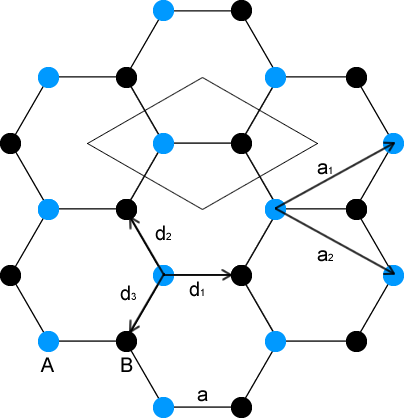
\includegraphics[scale=0.5]{images/strucure-zig-flat}}
					\caption{}
				\end{subfigure}
				\hspace{1cm}
				\begin{subfigure}[h]{0.47\textwidth}
					\centerline{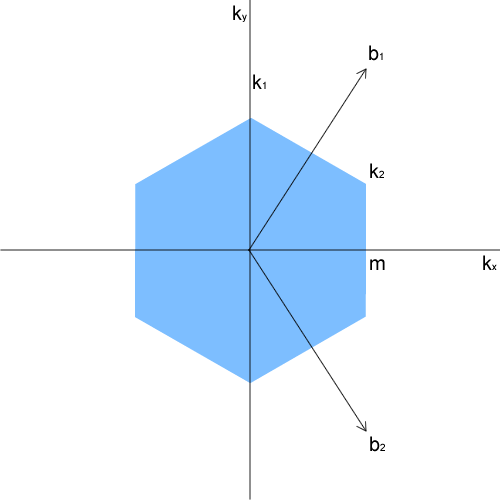
\includegraphics[scale=0.42]{images/strucure-bz-zig-flat}}
					\caption{}
				\end{subfigure}
				\caption{(a) The lattice vectors $\vec{a}_{1},\vec{a}_{2}$, nearest neighbor vectors $\vec{d}_{1},\vec{d}_{2},\vec{d}_{3}$, unit cell,  the carbon-carbon bond length $a=0.142$ nm and the sub lattices A and B. (b) The Brillouin zone with reciprocal lattice vectors $\vec{b}_{1},\vec{b}_{2}$, Dirac points $k_{1},k_{2}$ and point $m$.}
				\label{introduction-structure-zig}
			\end{figure}
			\begin{align}
				\vec{d}_{1}=a\left(1,0\right)\hspace{1cm}\vec{d}_{2}=\frac{a}{2}\left(-1,\sqrt{3}\right)\hspace{1cm}\vec{d}_{3}=\frac{a}{2}\left(-1,-\sqrt{3}\right)
			\end{align}
			Using the nearest neighbor vectors the lattice vectors can be found. These lattice vectors are for the individual triangular lattices and show the locations of the other atoms on the same lattice. To show the full hexagonal lattice these lattice vectors should start from an A and a B atom. The lattice vectors in zig-zag orientation are \cite{b1}:
			\begin{align}
				\vec{a}_{1}=\vec{d}_{1}-\vec{d}_{3}=\frac{a}{2}\left(3,\sqrt{3}\right)\hspace{1cm}\vec{a}_{2}=\frac{a}{2}\left(3,-\sqrt{3}\right)
			\end{align}
			The reciprocal lattice vectors are defined as:
			\begin{align}
				\vec{b}_{1}=2\pi\frac{\vec{a}_{2}\times\vec{a}_{z}}{\vec{a}_{1}\cdot\vec{a}_{2}\times\vec{a}_{z}}\hspace{1cm}\vec{b}_{2}=2\pi\frac{\vec{a}_{z}\times\vec{a}_{1}}{\vec{a}_{1}\cdot\vec{a}_{2}\times\vec{a}_{z}}
			\end{align}
			As graphene is two dimensional, the z components of $\vec{a}_{1}$ and $\vec{a}_{2}$ can be taken to be zero with $\vec{a}_{z}$ as the z direction unit vector. With the definitions of $\vec{a}_{1}$ and $\vec{a}_{2}$ the reciprocal lattice vectors become \cite{b1}:
			\begin{align}
				\vec{b_{1}}=\frac{2\pi}{3a}\left(1,\sqrt{3}\right)\hspace{1cm}\vec{b_{2}}=\frac{2\pi}{3a}\left(1,-\sqrt{3}\right)
			\end{align}
			In later sections the points where the valance and conduction bands meet will be studied, these are known as Dirac points. The locations of the Dirac points $k_{1}, k_{2}$ are at the corners of the Brillouin zone. Due to the symmetry of graphene only two Dirac points need to be found. Using the reciprocal lattice vectors and the half way point $m$:
			\begin{align}
				|m|=\frac{|\vec{b_{1}}|}{2}\hspace{1cm}|\vec{b_{1}}|=\sqrt{\left(\frac{2\pi}{3a}\right)^{2}+\left(\frac{2\pi\sqrt{3}}{3a}\right)^{2}}=\frac{4\pi}{3a}
			\end{align}
			the Dirac points can be found.
			\begin{align}
				k_{1}&=\left(0,\sqrt{\left(\frac{2\pi}{3a}\right)^{2}+\left(\frac{2\pi}{3a\sqrt{3}}\right)^{2}}\right)=\left(0,\frac{4\pi}{3\sqrt{3}a}\right)\\
				k_{2}&=\left(|m|,\frac{|m|}{\sin(\pi/3)}\sin(\pi/6)\right)=\left(\frac{2\pi}{3a},\frac{2\pi}{3a\sqrt{3}}\right)
			\end{align}
			The unit cell and all previously derived vectors for graphene have been included in Figure \ref{introduction-structure-zig}.
%%%%%
%%%%%
%%%%%
		\subsection{Armchair Orientation}
		\label{Introduction - Armchair Orientation}
			The same calculations can then be made to find the vectors for armchair orientation, this is a rotation of $30^{\circ}$, which can be useful as the $y$ component of $\vec{a}_{4}$ becomes zero.
			\begin{figure}[h]
				 \begin{subfigure}[h]{0.47\textwidth}
					\centerline{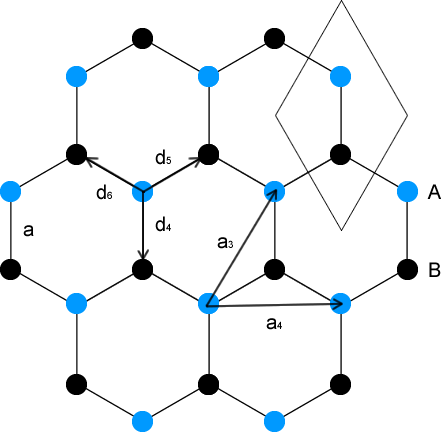
\includegraphics[scale=0.5]{images/strucure-arm-flat}}
					\caption{}
				\end{subfigure}
				\hspace{1cm}
				\begin{subfigure}[h]{0.47\textwidth}
					\centerline{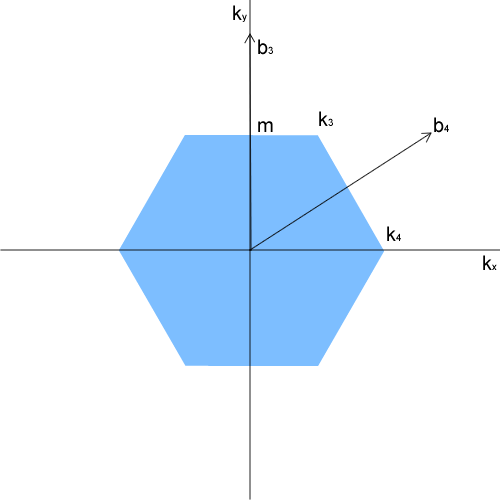
\includegraphics[scale=0.43]{images/strucure-bz-arm-flat}}
					\caption{}
				\end{subfigure}
				\caption{(a) The lattice vectors $\vec{a}_{3},\vec{a}_{4}$, nearest neighbor vectors $\vec{d}_{4},\vec{d}_{5},\vec{d}_{6}$, unit cell, the carbon-carbon bond length $a=0.142$ nm and the sub lattices A and B. (b) The Brillouin zone with reciprocal lattice vectors $\vec{b}_{3},\vec{b}_{4}$, Dirac points $k_{3},k_{4}$ and the mid point $m$.}
				\label{introduction-structure-armchair}
			\end{figure}
			The nearest neighbor vectors in this rotation are then \cite{b55}:
			\begin{align}
				\vec{d}_{4}=a\left(0,-1\right)
				\hspace{1cm}
				\vec{d}_{5}=\frac{a}{2}\left(\sqrt{3},1\right)
				\hspace{1cm}
				\vec{d}_{6}=\frac{1}{2}\left(-\sqrt{3},1\right)
			\end{align}
			with lattice vectors:
			\begin{align}
				\vec{a}_{3}=\frac{a}{2}\left(\sqrt{3},3\right)\hspace{1cm}\vec{a}_{4}=a\sqrt{3}\left(1,0\right)
			\end{align}
			reciprocal lattice vectors:
			\begin{align}
				\vec{b}_{3}=\frac{4\pi}{3a}\left(0,1\right)\hspace{1cm}\vec{b}_{4}=\frac{2\pi}{3a}\left(\sqrt{3},1\right)
			\end{align}
			and Dirac points:
			\begin{align}
				k_{3}=\frac{2\pi}{3a}\left(\frac{1}{\sqrt{3}},1\right)\hspace{1cm}k_{4}=\frac{4\pi}{3\sqrt{3}a}\left(1,0\right)
			\end{align}
			The unit cell and all other vectors for armchair graphene are shown in Figure \ref{introduction-structure-armchair}.
%%%%%
%%%%%
%%%%%
\section{Tight Binding Approximation}
\label{Introduction - Tight Binding Approximation}
	The tight binding approximation will reveal the full energy spectrum for the graphene hexagonal lattice. This is done by asigning each electron a Bloch wave-function and allowing it to hop to other atoms in the lattice. Other atoms are located using the lattice and neighbor vectors from Section \ref{Introduction - Structure}. In this section vectors for the zig-zag orientation will be used as shown in Figure \ref{introduction-tb-diagram} and derived in Section \ref{Introduction - Zig-Zag Orientation}. Depending on the range of hopping allowed; the accuracy of this approximation will increase.
	\begin{figure}[h]
		\begin{align}
			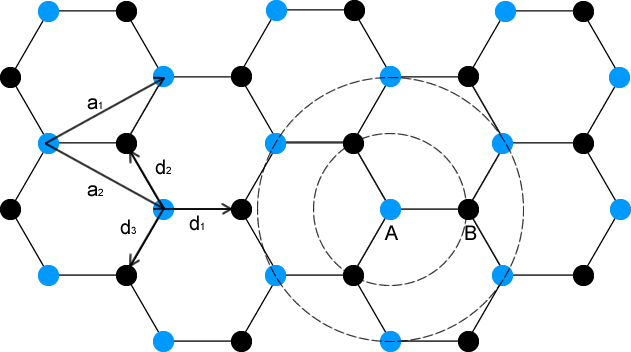
\includegraphics[scale=0.5]{images/tight-binding-flat}		
		\end{align}
		\caption{The graphene structure used for the tight binding approximation. The nearest neighbor vectors $\vec{d}_{1,2,3}$ and lattice vectors $\vec{a}_{1,2}$ have been included as defined in Section \ref{Introduction - Zig-Zag Orientation}. The radius for nearest neighbor and second nearest neighbor hopping is shown centered at an A site atom.}
		\label{introduction-tb-diagram}
	\end{figure}
%%%%%
%%%%%
%%%%%
	\subsection{Nearest Neighbor Only}
		\label{nearest-neighbor-only}
		Here only nearest neighbor hopping will be considered. This condition only allows hopping from A sites to B sites and vice versa. The Bloch wave-function \cite{b44} is defined as:
		\begin{equation}							 \psi_{k}\left(\vec{r}\right)=\sum\limits_{\vec{R}}e^{i\vec{k}\cdot\vec{R}}\left(b_{a}\varphi_{a}\left(\vec{r}+\vec{R}\right)+b_{b}\varphi_{b}\left(\vec{r}+\vec{R}\right)\right)
		\end{equation}
		Due to the symmetry of the graphene lattice all the wave-functions will be equivalent, however the interaction from a B site electron to an A site atom will be shifted by some vector $\vec{d}$, thus for an A site atom the wave-functions for an electron on the A lattice and B lattice can be defined as:
		\begin{align}
 			\varphi_{a}\left(\vec{r}\right)\equiv\varphi\left(\vec{r}\right)\hspace{1cm}\varphi_{b}\left(\vec{r}\right)\equiv\varphi\left(\vec{r}+\vec{d}_{1}\right)
		\end{align}
		The opposite will be true for a B site atom. For a B site atom the wave-functions for electrons from each lattice are defined as:
		\begin{align}
 			\varphi_{b}\left(\vec{r}\right)\equiv\varphi\left(\vec{r}\right)\hspace{1cm}\varphi_{a}\left(\vec{r}\right)\equiv\varphi\left(\vec{r}-\vec{d}_{1}\right)
		\end{align}
			The Schr{\" o}dinger equation can take the form:
			\begin{align}
				\langle\varphi_{a,b}|\hat{H}|\psi_{k}\rangle&=\varepsilon_{k}\langle\varphi_{a,b}|\psi_{k}\rangle\\
				\langle\varphi_{a,b}|(\hat{H}_{\mathrm{atomic}}+\Delta u)|\psi_{k}\rangle&=E\langle\varphi_{a,b}|\psi_{k}\rangle+\langle\varphi_{a,b}|\Delta u|\psi_{k}\rangle
			\end{align}
			Here the Schr{\" o}dinger equation has been split into the atomic component and an external potential; $\varepsilon_{k}$ is the energy of the whole system, $E$ is the energy of the atomic $p_{z}$ orbital electron and $\Delta u$ is an external potential. With this definition of the Schr{\" o}dinger equation and the previous definitions for electrons at A and B sites, the bra-kets can be evaluated, so for an A site:
			\begin{align}
				\langle\varphi_{a}|\psi_{k}\rangle=\sum\limits_{\vec{R}}e^{i\vec{k}\cdot\vec{R}}\left(b_{a}\int\varphi^{*}\left(\vec{r}\right)\varphi\left(\vec{r}+\vec{R}\right)d\vec{r}+b_{b}\int\varphi^{*}\left(\vec{r}\right)\varphi\left(\vec{r}+\vec{R}+\vec{d}_{1}\right)d\vec{r}\right)
				\label{introduction-start-tb}
			\end{align}
			Then for nearest neighbor atoms the vector $\vec{R}$ can only be:
			\begin{align}
				\vec{R}=0, -\vec{a}_{1}, -\vec{a}_{2}
			\end{align}
			Similarly for a B site:
			\begin{align}
				\langle\varphi_{b}|\psi_{k}\rangle=\sum\limits_{\vec{R}}e^{i\vec{k}\cdot\vec{R}}\left(b_{a}\int\varphi^{*}\left(\vec{r}\right)\varphi\left(\vec{r}+\vec{R}-\vec{d}_{1}\right)d\vec{r}+b_{b}\int\varphi^{*}\left(\vec{r}\right)\varphi\left(\vec{r}+\vec{R}\right)d\vec{r}\right)
				\label{introduction-start-tb-b}
			\end{align}
			and the vector $\vec{R}$:
			\begin{align}
				\vec{R}=0, \vec{a}_{1}, \vec{a}_{2}
			\end{align}
			Evaluating the sums and removing any terms which didn't reach atoms:
			\begin{align}
				\langle\varphi_{a}|\psi_{k}\rangle&=b_{a}\int\varphi^{*}\left(\vec{r}\right)\varphi\left(\vec{r}\right)d\vec{r}+b_{b}\int\varphi^{*}\left(\vec{r}\right)\varphi\left(\vec{r}+\vec{d}_{1}\right)d\vec{r}\\
				&+e^{-i\vec{k}\cdot\vec{a}_{1}}b_{b}\int\varphi^{*}\left(\vec{r}\right)\varphi\left(\vec{r}+\vec{d}_{3}\right)d\vec{r}+e^{-i\vec{k}\cdot\vec{a}_{2}}b_{b}\int\varphi^{*}\left(\vec{r}\right)\varphi\left(\vec{r}+\vec{d}_{2}\right)d\vec{r}\\
				\langle\varphi_{b}|\psi_{k}\rangle&=b_{a}\int\varphi^{*}\left(\vec{r}\right)\varphi\left(\vec{r}-\vec{d}_{1}\right)d\vec{r}+b_{b}\int\varphi^{*}\left(\vec{r}\right)\varphi\left(\vec{r}\right)d\vec{r}\\
				&+e^{i\vec{k}\cdot\vec{a}_{1}}b_{a}\int\varphi^{*}\left(\vec{r}\right)\varphi\left(\vec{r}-\vec{d}_{3}\right)d\vec{r}+e^{i\vec{k}\cdot\vec{a}_{2}}b_{a}\int\varphi^{*}\left(\vec{r}\right)\varphi\left(\vec{r}-\vec{d}_{2}\right)d\vec{r}
			\end{align}
			As the graphene sheet is symmetrical, the probability of an electron hopping from an A site to a B site will be the same as an electron hopping from a B site to an A site, this probability will be defined as:
			\begin{align}
				\int\varphi^{*}\left(\vec{r}\right)\varphi\left(\vec{r}-\vec{d}_{1,2,3}\right)d\vec{r}=\int\varphi^{*}\left(\vec{r}\right)\varphi\left(\vec{r}+\vec{d}_{1,2,3}\right)d\vec{r}\equiv\alpha
			\end{align}
			As $\int\varphi^{*}\left(\vec{r}\right)\varphi\left(\vec{r}\right)d\vec{r}$ must be equal to one from normalisation the bra-kets for A and B sites become:
			\begin{align}
				\langle\varphi_{a}|\psi_{k}\rangle&=b_{a}+b_{b}\alpha\left(1+e^{-i\vec{k}\cdot\vec{a}_{1}}+e^{-i\vec{k}\cdot\vec{a}_{2}}\right)\\
				\langle\varphi_{b}|\psi_{k}\rangle&=b_{b}+b_{a}\alpha\left(1+e^{i\vec{k}\cdot\vec{a}_{1}}+e^{i\vec{k}\cdot\vec{a}_{2}}\right)
			\end{align}
			The same method can be applied to $\langle\varphi_{a,b}|\Delta u|\psi_{k}\rangle$  with the definitions:
			\begin{align}
				\beta\equiv\int\varphi^{*}\left(\vec{r}\right)\Delta u\left(\vec{r}\right)\varphi\left(\vec{r}\right) d\vec{r}\hspace{1cm}t\equiv\int\varphi^{*}\left(\vec{r}\right)\Delta u\left(\vec{r}\right)\varphi\left(\vec{r}+\vec{d}_{1,2,3}\right) d\vec{r}
			\end{align}
			Which results in:
			\begin{align}
				\langle\varphi_{a}|\Delta u|\psi_{k}\rangle&=b_{a}\beta+b_{b}t\left(1+e^{-i\vec{k}\cdot\vec{a}_{1}}+e^{-i\vec{k}\cdot\vec{a}_{2}}\right)\\
				\langle\varphi_{b}|\Delta u|\psi_{k}\rangle&=b_{b}\beta+b_{a}t\left(1+e^{i\vec{k}\cdot\vec{a}_{1}}+e^{i\vec{k}\cdot\vec{a}_{2}}\right)
			\end{align}
			The previously derived values of $\vec{a}_{1}, \vec{a}_{2}$ can be used to define $f\left(\vec{k}\right)$ as:
			\begin{equation}
				f\left(\vec{k}\right)\equiv 1+e^{-i\vec{k}\cdot\vec{a}_{1}}+e^{-i\vec{k}\cdot\vec{a}_{2}}=1+2e^{-i\left(\frac{3ak_{x}}{2}\right)}\cos\left(\frac{\sqrt{3}ak_{y}}{2}\right)
				\label{introduction-fk}
			\end{equation}
			With the bra-kets evaluated the total energy of the system $\varepsilon_{k}\langle\varphi_{a,b}|\psi_{k}\rangle=E\langle\varphi_{a,b}|\psi_{k}\rangle+\langle\varphi_{a,b}|\Delta u|\psi_{k}\rangle$ can be written as:
			\begin{align}
				b_{a}\left(\varepsilon_{k}-E+\beta\right)+b_{b}f\left(\vec{k}\right)\left(\left(\varepsilon_{k}-E\right)\alpha+t\right)&=0\\
				b_{b}\left(\varepsilon_{k}-E+\beta\right)+b_{a}f^{*}\left(\vec{k}\right)\left(\left(\varepsilon_{k}-E\right)\alpha+t\right)&=0
			\end{align}
			Since $\Delta u\left(\vec{r}\right)$ will be large at $\vec{r}+\vec{d}_{1}$, it can be assumed that $\varphi\left(\vec{r}+\vec{d}_{1}\right)\ll\Delta u\left(\vec{r}\right)\varphi\left(\vec{r}+\vec{d}_{1}\right)$ and therefore $\alpha\ll t$ and $\alpha=0$. These simultaneous equations can then be written in matrix from:
			\begin{align}
				\left[\begin{array}{ccc}
					\varepsilon_{k}-E+\beta&t f\left(\vec{k}\right)\\
					t f^{*}\left(\vec{k}\right)&\varepsilon_{k}-E+\beta
				\end{array}\right]
				\left[\begin{array}{ccc}
					b_{a}\\
					b_{b}	
				\end{array}\right]=
				\left[\begin{array}{ccc}
					0\\
					0
				\end{array}\right]
			\end{align}
			The quantities $E$ and $\beta$ have no dependence on $\vec{k}$ therefore these values will only shift the spectrum and can be set to zero. The energy eigenvalues of this matrix can then be found:
			\begin{align}
				\hat{H}=\left[\begin{array}{ccc}
					\varepsilon_{k}&t f\left(\vec{k}\right)\\
					t f^{*}\left(\vec{k}\right)&\varepsilon_{k}
				\end{array}\right]
				\hspace{1cm}
				\det\left(\hat{H}\right)=0
			\end{align}
			Showing the full symmetrical energy spectrum from the nearest neighbor only tight binding approximation:
			\begin{align}
				\varepsilon_{\pm}\left(\vec{k}\right)=\pm t|f\left(\vec{k}\right)|
				\label{introduction-ek}
			\end{align}
			A plot of Equation (\ref{introduction-ek}) can be seen in Figure \ref{introduction-fk-plot}. The value of $t$ is the hopping energy and $|f\left(\vec{k}\right)|$ can be evaluated as \cite{b8,b11}:
			\begin{align}
				|f\left(\vec{k}\right)|=\sqrt{3+2\cos\left(\sqrt{3}ak_{y}\right)+4\cos\left(\frac{3}{2}ak_{x}\right)\cos\left(\frac{\sqrt{3}}{2}ak_{y}\right)}
				\label{mod-fk}
			\end{align}
			\begin{figure}[h]
				\centerline{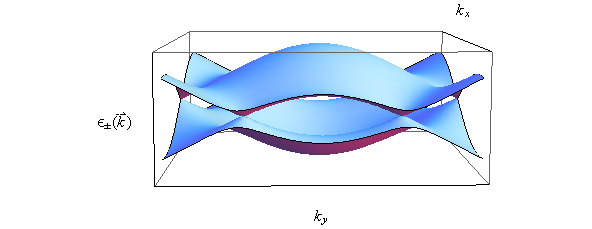
\includegraphics[scale=0.6]{images/tight-binding}}	
				\caption{A three dimensional plot of the full energy spectrum for a hexagonal graphene sheet from Equation (\ref{mod-fk}). This plot clearly shows the Dirac points located at the corners of the Brillouin zone.}
				\label{introduction-fk-plot}
			\end{figure}
%%%%%
%%%%%
%%%%%
		\subsection{Second Nearest Neighbor}
		\label{Introduction - Second Nearest Neighbor}
			To include second nearest neighbor hopping the method is similar and can be taken to be the same until Equation (\ref{introduction-start-tb}). The vector $\vec{R}$ must then be expanded to include the next A lattice atoms and becomes:
			\begin{align}
				\vec{R}=0, \vec{a}_{1}, \vec{a}_{2}, -\vec{a}_{1}, -\vec{a}_{2}, \vec{a}_{1}-\vec{a}_{2}, \vec{a}_{2}-\vec{a}_{2}
			\end{align}
			Evaluating the sum in Equation (\ref{introduction-start-tb}) with the new vector $\vec{R}$:
			\begin{align}
				\langle\varphi_{a}|\psi_{k}\rangle&=b_{a}+b_{b}\alpha f\left(\vec{k}\right)+b_{a}\alpha_{2}\left(e^{i\vec{k}\cdot\vec{a}_{1}}+e^{i\vec{k}\cdot\vec{a}_{2}}+e^{-i\vec{k}\cdot\vec{a}_{1}}+e^{-i\vec{k}\cdot\vec{a}_{2}}+e^{i\vec{k}\cdot\left(\vec{a}_{1}-\vec{a}_{2}\right)}+e^{i\vec{k}\cdot\left(\vec{a}_{2}-\vec{a}_{1}\right)}\right)\\
				&=b_{a}+b_{b}\alpha f\left(\vec{k}\right)+2b_{a}\alpha_{2}\left(\cos\left(\vec{k}\cdot \vec{a}_{1}\right)+\cos\left(\vec{k}\cdot \vec{a}_{2}\right)+\cos\left(\vec{k}\cdot \vec{a}_{1}-\vec{k}\cdot \vec{a}_{2}\right)\right)\\
				&=b_{a}+b_{b}\alpha f\left(\vec{k}\right)+b_{a}\alpha_{2}g\left(\vec{k}\right)
			\end{align}
			Where $g\left(\vec{k}\right)$ has been defined as:
			\begin{align}
				g\left(\vec{k}\right)&=2\left(\cos\left(\vec{k}\cdot \vec{a}_{1}\right)+\cos\left(\vec{k}\cdot \vec{a}_{2}\right)+\cos\left(\vec{k}\cdot \vec{a}_{1}-\vec{k}\cdot \vec{a}_{2}\right)\right)\\
				&=2\cos\left(\sqrt{3}ak_{y}\right)+4\cos\left(\frac{3}{2}ak_{x}\right)\cos\left(\frac{\sqrt{3}}{2}ak_{y}\right)
			\end{align}
			and:
			\begin{align}
				\alpha_{2}=\int\varphi^{*}\left(\vec{r}\right)\varphi\left(\vec{r}+\vec{a}_{1,2}\right)d\vec{r}
			\end{align}
			Then with Equation (\ref{introduction-start-tb-b}), the new vector $\vec{R}$ centered at a B site will find all second nearest neighbors and therefore is the same as the A site, so evaluating the sum:
			\begin{align}
				\langle\varphi_{b}|\psi_{k}\rangle=b_{b}+b_{a}\alpha f^{*}\left(\vec{k}\right)+b_{b}\alpha_{2}g\left(\vec{k}\right)
			\end{align}
			Then evaluating $\langle\varphi_{a,b}|\Delta u|\psi_{k}\rangle$:
			\begin{align}
				\langle\varphi_{a}|\Delta u|\psi_{k}\rangle&=b_{a}\beta+b_{b}tf\left(\vec{k}\right)+b_{a}t'g\left(\vec{k}\right)\\
				\langle\varphi_{b}|\Delta u|\psi_{k}\rangle&=b_{b}\beta+b_{a}tf^{*}\left(\vec{k}\right)+b_{b}t'g\left(\vec{k}\right)
			\end{align}
			with the definition:
			\begin{align}
				t'\equiv\int\varphi^{*}\left(\vec{r}\right)\Delta u\left(\vec{r}\right)\varphi\left(\vec{r}+\vec{a}_{1,2}\right) d\vec{r}
			\end{align}
			The total energy of the system, including hopping from second nearest neighbors can now be written as a set of simultaneous equations:
			\begin{align}
				b_{a}\left(\varepsilon_{k}+\varepsilon_{k}\alpha_{2}g\left(\vec{k}\right)-E-\alpha_{2}g\left(\vec{k}\right)-\beta-t'g\left(\vec{k}\right)\right)+b_{b}f\left(\vec{k}\right)\left(\varepsilon_{k}\alpha-E\alpha-t\right)&=0\\
				b_{a}f^{*}\left(\vec{k}\right)\left(\varepsilon_{k}\alpha-E\alpha-t\right)+b_{b}\left(\varepsilon_{k}+\varepsilon_{k}\alpha_{2}g\left(\vec{k}\right)-E-\alpha_{2}g\left(\vec{k}\right)-\beta-t'g\left(\vec{k}\right)\right)&=0
			\end{align}
			Due to similar conditions as the nearest neighbor only case; $\alpha=0$, $\alpha_{2}=0$, $E=0$, $\beta=0$. In matrix form these equations become:
			\begin{align}
				\hat{H}=\left[\begin{array}{ccc}
					-\varepsilon_{k}+t'g\left(\vec{k}\right)&t f\left(\vec{k}\right)\\
					t f^{*}\left(\vec{k}\right)&-\varepsilon_{k}+t'g\left(\vec{k}\right)
				\end{array}\right]\hspace{1cm}\det\left(\hat{H}\right)=0
			\end{align}
			Which produces the eigenvalue:
			\begin{align}
				\varepsilon_{\pm}\left(\vec{k}\right)=t'g\left(\vec{k}\right)\pm t\sqrt{3+g\left(\vec{k}\right)}
				\label{fk-second}
			\end{align}
			A plot of this energy spectrum can be seen in Figure \ref{introduction-fk-plot-second}. This plot shows the energy spectrum has become asymmetrical around the Fermi level \cite{b1}, however maintains the Dirac points at the corners of the Brillouin zone.
			\begin{figure}[h]
				\centerline{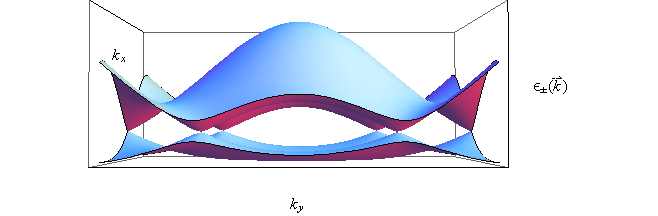
\includegraphics[scale=0.6]{images/tb-second}}
				\caption{A three dimensional plot of the full energy spectrum for a hexagonal graphene sheet from Equation (\ref{fk-second}) including second nearest neighbor hopping. The inclusion of the second nearest neighbor hopping breaks the symmetry for electrons and holes.}
				\label{introduction-fk-plot-second}
			\end{figure}
%%%%%
%%%%%
%%%%%
		\section{Hamiltonian}
		\label{Introduction - Hamiltonian}
			A two variable Taylor expansion around a Dirac point will produce the Hamiltonian for quasiparticles at a Dirac point. This is done by first setting $\vec{k}\rightarrow \vec{k_{2}}+\vec{j}$, where $\vec{k_{2}}$ was derived in Section \ref{Introduction - Zig-Zag Orientation}. With this adjustment the momentum becomes:
			\begin{equation}
				\vec{k}=\left(\frac{2\pi}{3a}+j_{x},\frac{2\pi}{3\sqrt{3}a}+j_{y}\right)
				\label{kpoint}
			\end{equation}
			The full energy spectrum from Section \ref{nearest-neighbor-only} becomes:
			\begin{align}
				f\left(\vec{k}\right)&=1+2e^{-i\left(\frac{3a}{2}\left(k_{x}+j_{x}\right)\right)}\cos\left(\frac{\sqrt{3}a}{2}\left(k_{y}+j_{y}\right)\right)\\
				&=1+2e^{-i\left(\frac{3a}{2}j_{x}\right)}\cos\left(\frac{2\pi}{3}+\frac{\sqrt{3}a}{2}j_{y}\right)\\
				&=1+e^{-i\frac{3a}{2}j_{x}}\left(\cos\left(\frac{\sqrt{3}a}{2}j_{y}\right)-\sqrt{3}\sin\left(\frac{\sqrt{3}a}{2}j_{y}\right)\right)
			\end{align}
			By performing a two variable Taylor expansion around the point $\left(k_{x}, k_{y}\right)$ an approximation of $f(\vec{k})$ and $f^{*}(\vec{k})$ can be made around the region of a Dirac point. The first order, two variable Taylor expansion around point $a$,$b$ is defined as:
			\begin{align}
				f\left(x,y\right)=f\left(a,b\right)+\left(x-a\right)f'_{x}\left(a,b\right)+\left(y-b\right)f'_{y}\left(a,b\right)
			\end{align}
			Applying this to $f\left(k_{x},k_{y}\right)$ produces:
			\begin{align}
				f\left(k_{x},k_{y}\right)&=f\left(j_{x},j_{y}\right)+\left(k_{x}-j_{x}\right)f'_{x}\left(j_{x},j_{y}\right)+\left(k_{y}-j_{y}\right)f'_{y}\left(j_{x},j_{y}\right)\\
				f'_{x}\left(j_{x},j_{y}\right)&=-i\frac{3a}{2}e^{-i\frac{3a}{2}j_{x}}\left(\cos\left(\frac{\sqrt{3}a}{2}j_{y}\right)-\sqrt{3}\sin\left(\frac{\sqrt{3}a}{2}j_{y}\right)\right)\\
				f'_{y}\left(j_{x},j_{y}\right)&=e^{-i\frac{3a}{2}j_{x}}\left(-\frac{\sqrt{3}a}{2}\sin\left(\frac{\sqrt{3}a}{2}j_{y}\right)-\frac{3a}{2}\cos\left(\frac{\sqrt{3}a}{2}j_{y}\right)\right)
			\end{align}
			Setting $\vec{j}=0$  centers the expansion around a Dirac point; $f(\vec{k})$ and $f^{*}(\vec{k})$ become:
			\begin{align}
				f\left(k_{x}, k_{y}\right)=-i\frac{3a}{2}k_{x}-\frac{3a}{2}k_{y}
				\hspace{1cm}
				f^{*}\left(k_{x}, k_{y}\right)=i\frac{3a}{2}k_{x}-\frac{3a}{2}k_{y}
				\label{fofk}
			\end{align}
			These can then be substituted into the whole spectrum to find the Hamiltonian at a Dirac point.
			\begin{align}
				\hat{H}=
				\left[\begin{array}{ccc}
					\varepsilon_{k}&t\left(-i\frac{3a}{2}k_{x}-\frac{3a}{2}k_{y}\right)\\
					t\left(i\frac{3a}{2}k_{x}-\frac{3a}{2}k_{y}\right)&\varepsilon_{k}
				\end{array}\right]
			\end{align}
			$\varepsilon_{k}$ can be set to zero to center the spectrum at the Fermi level. The result here is produced from the vectors in Section \ref{Introduction - Zig-Zag Orientation}, in order to obtain the result for the 2x2 Hamiltonian in \cite{b2,b4} different rotations of the lattice vectors are needed. The standard graphene Hamiltonian is given as:
			\begin{align}
				\hat{H}=v_{f}\sigma_{x,y}\cdot\hat{p}+\sigma_{z}m
				\hspace{1cm}
				v_{f}=\frac{3at}{2\hbar}=\frac{c}{300}
				\hspace{1cm}
				\hat{p}=-i\hbar\bigtriangledown
				\hspace{1cm}
				m=m_{0}v_{f}^{2}
				\label{introduction - hamiltonian eq}
			\end{align}
			Where $a=0.142$ nm \cite{b8}, the hopping energy $t=2.8$ eV \cite{b1}, $m_{0}$ is a mass term \cite{b47} and $c$ is the speed of light in a vacuum. The Hamiltonian can be expanded into matrix form using the Pauli matrices:
			\begin{align}
				\sigma_{x}=
				\left[\begin{array}{ccc}
					0&1\\
					1&0
				\end{array}\right]
				\hspace{1cm}\sigma_{y}=
				\left[\begin{array}{ccc}
					0&-i\\
					i&0
				\end{array}\right]
				\hspace{1cm}\sigma_{z}=
				\left[\begin{array}{ccc}
					1&0\\
					0&-1
				\end{array}\right]
			\end{align}
			and the definition of momentum operator to produce:
			\begin{align}
				\hat{H}=\left[\begin{array}{ccc}
					m&-\hbar v_{f}\left(i\frac{\partial}{\partial x}+\frac{\partial}{\partial y}\right)\\
					-\hbar v_{f}\left(i\frac{\partial}{\partial x}-\frac{\partial}{\partial y}\right)&-m
				\end{array}\right]
			\end{align}
			By using a different Dirac point, known as a $k'$ point instead of Equation (\ref{kpoint}) the two by two Hamiltonian for the $k'$ point can also be found. The two sets of simultaneous equations can then be combined to form the four by four Hamiltonian:
			\begin{align}
				\hat{H}=\hbar v_{f}\left[\begin{array}{cccc}
					m/\hbar v_{f}&k_{x}+ik_{y}&0&0\\
					k_{x}-ik_{y}&-m/\hbar v_{f}&0&0\\
					0&0&-m/\hbar v_{f}&-k_{x}-ik_{y}\\
					0&0&-k_{x}+ik_{y}&m/\hbar v_{f}
				\end{array}\right]
			\end{align}
			This matrix is directly comparable to the Hamiltonian derived from gamma matrices for the Dirac equation or inverted band structure heterojunctions \cite{b41}. This combined with the near relativistic Fermi velocity makes graphene an ideal candidate for use with the Dirac equation for relativistic particles. However since the non-zero sub matricies are essentially negatives of eachother, for simplicity the two by two Hamiltonian is often used. If results for the four by four Hamiltonian are required they are easily obtained from the two by two Hamiltonian.
%%%%%
%%%%%
%%%%%
		\section{Dispersion relation at Dirac points}
		\label{Introduction - Dispersion relation at Dirac points}
			By finding the eigenvalue of the graphene Hamiltonian, the dispersion relation for graphene at a Dirac point can be found.
			\begin{align}
				\det\left(\hat{H}-E\right)=0\hspace{1cm}E=\pm\sqrt{\hbar^{2}v_{f}^{2}\left(k_{x}^{2}+k_{y}^{2}\right)+m^{2}}
				\label{introduction-ekm}
			\end{align}
			This produces a Dirac cone when $m=0$ \cite{b5, b55} showing the conduction and valance band touching at a Dirac point. The energy spectrum with a mass term \cite{b46, b47, b4, b55} becomes parabolic with a gap between the conduction and valance band equivalant to $2m$. This gap may be formed in zig-zag type nanoribbons \cite{b1}, the application of strain \cite{b59}, by interaction with a substrate and by transverse electric field \cite{b47} in situations when inversion symmetry is broken.

			\begin{figure}[h]
				 \begin{subfigure}[h]{0.45\textwidth}
					\centerline{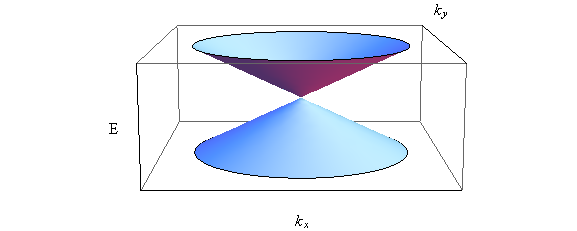
\includegraphics[scale=0.5]{images/dispersion}}
					\caption{$m=0$}
				\end{subfigure}
				\hspace{1cm}
				\begin{subfigure}[h]{0.45\textwidth}
					\centerline{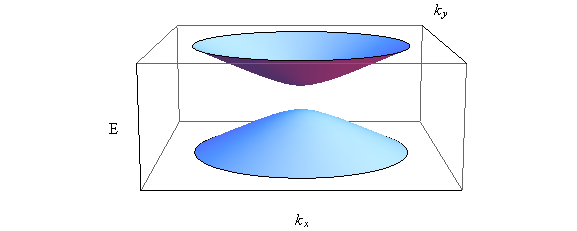
\includegraphics[scale=0.5]{images/dispersion-m}}
					\caption{$m\ne 0$}
				\end{subfigure}
				\caption{The energy momentum relation near a Dirac point from Equation (\ref{introduction-ekm}). In (a) the gapless spectrum shows a Dirac cone with the energy bands touching at a Dirac point. In (b) graphene has a parabolic energy spectrum with an energy gap of $2m$ between the energy bands.}
			\end{figure}
%%%%%
%%%%%
%%%%%
%		\section{Zener Tunnelling}
%		\label{Introduction - Zener Tunnelling}
%The linear dispersion relation that allows for Klein tunnelling through potential barriers also makes graphene an ideal candidate for Zener tunnelling devices. Zener tunnelling is the process whereby an electron may be excited from the valence band into the conduction band by a strong electric field \cite{b42,b43}. In this section the rate at which electrons may jump from the valence band will be determined using the methods outlined in \cite{b42}.
%
%		For a one dimensional lattice, the potential energy of the electron is represented by $V\left(x\right)$ with a period $a$. The wave equation of a periodic potential has solutions in the form of a Bloch wave-function \cite{b44}. 
%		\begin{equation}
%			\psi_{k}=e^{ikx}U_{k}\left(x\right)
%		\end{equation}
%		where the function $U_{k}\left(x\right)$ has the same period as $V\left(x\right)$, $a=2\pi/k$. The condition that the wave-function must be finite for all values of $x$ requires that $k$ is real when the enregy $E_{k}$ is within the allowed energy bands. The periodicity of the wave-function requires that the first energy band lies within the interval $-\pi/a \leq k \leq \pi/a$.
%		If an electric field $F$ is present, the wave-function $\psi\left(x,t\right)$ is expanded in terms of wave-functions of the lowest energy band when $F=0$:
%		\begin{equation}
%			\psi\left(x,t\right)=\int^{\pi/a}_{-\pi/a}g\left(k,t\right)\psi_{k}dk
%		\end{equation}
%		If transitions are only allowed for the first of each energy band the continuity equation:
%		\begin{equation}
%			\frac{d}{dt}|g|^{2}+\frac{2\pi eF}{h}|g|^{2}=0
%		\end{equation}
%		requires that $|g|^{2}$ is a function of $k$ and $t$ so that:
%		\begin{equation}
%			|g|^{2}=G\left(k-\frac{2\pi eF}{h}t\right)
%		\end{equation}
%		where $G$ is an arbitary function. With the periodic boundary of $\psi_{-\pi/a}=\psi_{\pi/a}$, $|g|^{2}$ must also be periodic with $t$. The frequency can then be calculated from $f=v/\lambda$ where:
%		\begin{align}
%			\lambda=\frac{2\pi}{a}\hspace{1cm}v=\frac{2\pi eF}{h}\hspace{1cm}f=\frac{eFa}{h}
%		\end{align}
%		To calculate the probability per unit time $\gamma$, that an electron will be excited into the conduction band the frequency of the wave packet must be multiplied by the probability of tunelling $p$.
%		\begin{equation}
%			\gamma = fp
%		\end{equation}
%		In order to calculate $p$, a wave-function periodic in time can be use with the wave equation:
%		\begin{equation}
%			\left(\frac{h^{2}}{8\pi^{2}m}\frac{d^{2}}{dx^{2}}-V\left(x\right)+\left(E-eFx\right)\right)\psi=0
%			\label{zener-wave}
%		\end{equation}
%		Assuming that $eFx$ does not vary much between atoms, the solution can be chosen to be in the form of:
%		\begin{equation}
%			\psi=e^{i\int K dx}U_{K}\left(x\right)
%			\label{zener-psi}
%		\end{equation}
%		where $K$ is a function of $\left(E-eFx\right)$ and $U_{K}$ is identical to the previous $U_{k}$ with $k=K$. With this defintion, $K$ will only become real with certain values of $E$ and $x$. If $K$ becomes imaginary the wave-function in Equation.(\ref{zener-psi}) will begin to decay. In each allowed energy band in Figure \ref{zener-flat} the wave-functions for electrons should be in the same oscillatory form, with decaying probability in the gap region. With oscillatory wave-functions in regions AB, CD and decaying wave-functions in region BC the transition probability $p$ between bands is given as:
%		\begin{equation}
%			p=|\psi_{CD}/\psi_{AB}|^{2}
%		\end{equation}
%
%\begin{figure}
%	\centerline{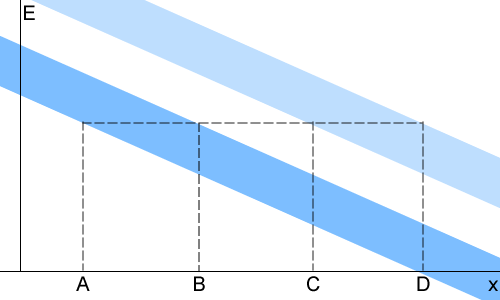
\includegraphics[scale=0.6]{images/zener-flat}}
%	\caption{Diagram of energy bands in a dielectric material in an electric field. The valence band (dark) and conduction band (light) are separated by a forbidden energy gap.}
%	\label{zener-flat}
%\end{figure}
%		
%		To allow Equation.(\ref{zener-psi}) to be either oscillatory or decaying, $K$ can be expressed as it's real and imaginary components:
%		\begin{equation}
%			K=\xi\left(x\right)+i\eta\left(x\right)
%		\end{equation}
%		As the wave-function must decay within the disallowed region, the probability must be in the form of exponential decay within region BC. This results in the probability:
%		\begin{equation}
%			|\psi_{CD}/\psi_{AB}|=e^{-\int^{C}_{B}\eta\left(x\right)dx}
%		\end{equation}
%		and the probability per unit time is then:
%		\begin{equation}
%			\gamma=\frac{eFa}{h}e^{-2\int^{C}_{B}\eta\left(x\right)dx}
%			\label{zener-gamma}
%		\end{equation}
%		To obtain an expression for $K$, the wave equation can be expressed as Hill's equation, in general form:
%		\begin{equation}
%			\frac{d^{2}}{dx^{2}}\psi+\left(\theta_{0}+2\Sigma_{n}\theta_{n}cos\left(2nx\right)\right)\psi=0
%		\end{equation}
%		This can be constructed with the substitutions $s=\pi x/a$ and $\theta_{0}=8ma^{2}(E-eFx)/h^{2}$ to Equation.(\ref{zener-wave}), resulting in:
%		\begin{equation}
%			\frac{d^{2}}{ds^{2}}\psi+\left(\theta_{0}+\frac{8ma^{2}}{h^{2}}V\left(x\right)\right)\psi=0
%		\end{equation}
%		The remaining terms are obtained by a Fourier series of $V(x)$. The Fourier series is defined as:
%		\begin{equation}
%			f\left(x\right)=\frac{1}{2}a_{0}+\sum\limits_{n=1}^{\infty}a_{a}cos\left(nx\right)+\sum\limits_{n=1}^{\infty}b_{n}sin\left(nx\right)
%		\end{equation}
%		where:
%		\begin{align}
%			a_{0}&=\frac{1}{\pi}\int^{\pi}_{-\pi}f\left(x\right)dx\\
%			a_{n}&=\frac{1}{\pi}\int^{\pi}_{-\pi}f\left(x\right)cos\left(nx\right)dx\\
%			b_{n}&=\frac{1}{\pi}\int^{\pi}_{-\pi}f\left(x\right)sin\left(nx\right)dx
%		\end{align}
%		As $V(x)$ must be a periodic function, the integration rules:
%		\begin{align}
%			&\int^{\pi}_{-\pi}sin\left(mx\right)sin\left(nx\right)dx=\pi \delta_{mn}
%			\hspace{1cm}			
%			&&\int^{\pi}_{-\pi}cos\left(mx\right)cos\left(nx\right)dx=\pi \delta_{mn}\\
%			&\int^{\pi}_{-\pi}cos\left(mx\right)sin\left(nx\right)dx=0
%			\hspace{1cm}
%			&&\int^{\pi}_{-\pi}sin\left(mx\right)cos\left(nx\right)dx=0\\
%			&\int^{\pi}_{-\pi}cos\left(mx\right)dx=0
%			\hspace{1cm}
%			&&\int^{\pi}_{-\pi}sin\left(mx\right)dx=0
%		\end{align}
%		can be used, with a potential of form $V(x)=cos(nx)$ with $x=sa/\pi$ and $a=2\pi$ to produce the equation:
%		\begin{equation}
%			\frac{d^{2}}{ds^{2}}\psi+\left(\theta_{0}+2\Sigma_{n}\theta_{m}cos\left(2ns\right)\right)\psi=0
%			\label{zener-hill}
%		\end{equation}
%		Where $\theta_{m}=4ma^{2}/h^{2}\theta_{n}$ from the fourier expansion. From the solution of Equation.(\ref{zener-hill}) in \cite{b45} the value of $K$ can be expressed in the form:
%		\begin{equation}
%			sin^{2}\left(aK/2\right)=sin^{2}\left(\frac{1}{2}\pi\sqrt{\theta_{0}}\right)\left(1+\frac{\pi\theta_{1}^{2}}{4\sqrt{\theta_{0}}\left(1-\theta_{0}\right)}cot\left(\pi\sqrt{\theta_{0}}/2\right)\right)+O\left(\theta_{1}^{4}\right)
%			\label{zener-hill-result}
%		\end{equation}
%		In the energy region that produces an imaginary $K$, $\theta_{0}$ will only be close to one and therefore $K$ will be approximately equal to $\pi\theta_{0}^{\frac{1}{2}}/2$ or $\pi/2$. With these conditions, the values:
%		\begin{align}
%			\theta_{0}&=1+\alpha \\
%			K&=\pi/2 + \beta
%		\end{align}
%		can be set, where $\alpha$ and $\beta$ are a small deviation. Using these values for $K$ and $\theta_{0}$ with Equation.(\ref{zener-hill-result}) produces the result for $K$:
%		\begin{equation}
%			K=\pi/a \pm i\left(\pi/a\right)\sqrt{\theta_{1}^{2}-\alpha^{2}}
%		\end{equation}
%		With the axis origin set between the points B and C, $K$ can be expressed as:
%		\begin{equation}
%			K=\frac{\pi}{a}\left(1\pm i\frac{8ma^{2}}{h^{2}}\left(V_{0}^{2}-\left(eFx\right)^{2}\right)^{\frac{1}{2}}\right)
%		\end{equation}
%		then with the integration in Equation.(\ref{zener-gamma}) between the points $B=V_{0}/eF$ and $C=-V_{0}/eF$ the rate of transmission becomes:
%		\begin{equation}
%			\gamma=\frac{eFa}{h}e^{-\frac{\pi^{2}}{h^{2}}\frac{ma\epsilon^{2}}{|eF|}}
%		\end{equation}
%		Where the size of the energy gap $\epsilon=2V_{0}$.
%%%%%
%%%%%
%%%%%

	\section{Wave-functions}
	\label{Wave-functions}
		The eigenvectors of the matrix Hamiltonian in Equation (\ref{introduction - hamiltonian eq}) can be used as the wave-functions for quasiparticles in graphene. In this section two types of wave-function will be derived. The oscillatory type wave-function is of the form of a plane wave and is useful for finding the properties of scattering devices. The other type of wave-function derived here is of the form of exponential growth or decay. These wave-functions are useful for finding localised states, where the particle is restricted to a specific region.
			\subsection{Oscillatory}
			\label{Wave-functions - Oscillitary}
			By applying the Hamiltonian to the Dirac equation wave-functions can be found for an infinite graphene sheet. With a potential and an energy gap the time independent Dirac equation takes the form:
			\begin{align}
				\left[\begin{array}{ccc}
				V-E+m&v_{f}\left(\hat{p}_{x}+i\hat{p}_{y}\right)\\
				v_{f}\left(\hat{p}_{x}-i\hat{p}_{y}\right)&V-E-m
				\end{array}\right]
				\left[\begin{array}{ccc}
				\psi_a\\
				\psi_b
				\end{array}\right]
				=0
			\end{align}
			To find non-trivial solutions, this can then be split into a system of simultaneous equations:
			\begin{equation}\label{eq:4}
				\left(V-E+m\right)\psi_{a}+ v_{f}\left(\hat{p}_{x}+i\hat{p}_{y}\right)\psi_{b}=0
			\end{equation}
			\begin{equation}\label{eq:5}
				\left(V-E-m\right)\psi_{b}+v_{f}\left(\hat{p}_{x}-i\hat{p}_{y}\right)\psi_{a}=0
			\end{equation}
			By making $\psi_{b}$ the subject of Equation (\ref{eq:5}), Equation (\ref{eq:4}) can take the form:
			\begin{equation}
				\frac{\left(E-V\right)^{2}-m^{2}}{\hbar^{2}v_{f}^{2}}\psi_{a}=\left(-\frac{\partial^{2}}{\partial x^{2}}-\frac{\partial^{2}}{\partial y^{2}}\right)\psi_{a}
				\label{eq:6}
			\end{equation}
			Since $V=V(x)$ and is independent of $y$, one can look for separable solutions $\psi_{a}(x,y)=f(x)g(y)$. Equation (\ref{eq:6}) then becomes:
			\begin{equation}
				\frac{1}{g(y)}\frac{d^{2}}{dy^{2}}g(y)=-\frac{\left(E-V\right)^{2}-m^{2}}{\hbar^{2}v_{f}^{2}}-\frac{1}{f(x)}\frac{d^{2}}{dx^{2}}f(x).
			\end{equation}
			%Requiring the wave-functions are separable means the wave-functions should be of the form $f\left(x\right)e^{ik_{y}y}$. Evaluating the derivitives with respect to $y$ produces the equation:
			Looking for plane wave solutions $g(y)\sim e^{ik_{y}y}$ gives 
			\begin{equation}
				q^{2}f\left(x\right)=-\frac{d^{2}}{d x^{2}}f\left(x\right),
			\end{equation}
			with the definition:
			\begin{equation}
				q^{2}=\frac{\left(E-V\right)^{2}-m^{2}}{\hbar^{2}v_{f}^{2}}-k_{y}^{2}
			\end{equation}
			A suitable solution of this equation produces the wave-function component:
			\begin{equation}
				\psi_{a}\left(x,y\right)=\left(a_{1}e^{iqx}+a_{2}e^{-iqx}\right)e^{ik_{y}y}
			\end{equation}
			Using the value for $\psi_{a}$, the wave-function component $\psi_{b}$ can be found with Equation (\ref{eq:5}):
			\begin{equation}
				\psi_{b}=\frac{\hbar v_{f}}{E-V+m}\left(-i\frac{\partial}{\partial x}+\frac{\partial}{\partial y}\right)\left(a_{1}e^{iqx}+a_{2}e^{-iqx}\right)e^{ik_{y}y}
			\end{equation}
			Evaluating this with:
			\begin{align}
				q=|\vec{q}|\cos(\theta)
				\hspace{1cm}
				k_{y}=|\vec{q}|\sin(\theta)\hspace{1cm}|\vec{q}|=\sqrt{q^{2}+k_{y}^{2}}=\sqrt{\frac{\left(E-V\right)^{2}-m^{2}}{\hbar^{2}v_{f}^{2}}}
			\end{align}
			Results in the final form of the wave-function component:
			\begin{equation}
				\psi_{b}=\alpha\left(a_{1} e^{iqx+i\theta}-a_{2} e^{-iqx-i\theta}\right)e^{ik_{y}y}
			\end{equation}
			Where constants have been grouped so that:
			\begin{align}
				\alpha=\frac{\sqrt{\left(E-V\right)^{2}-m^{2}}}{E-V+m}
			\end{align}
			Finally with normalisation the wave-functions for graphene with an energy gap and a potential can be stated to be:
			\begin{align}
				\psi\left(x,y\right)=
				c_{n}e^{ik_{y}y}
				\left[\begin{array}{ccc}
					e^{iqx}&e^{-iqx}\\
					\alpha e^{iqx+i\theta}&-\alpha e^{-iqx-i\theta}
				\end{array}\right]
				\left[\begin{array}{ccc}
					a_{1}\\
					a_{2}
				\end{array}\right]
				\label{introduction-wf}
			\end{align}
			where the normalisation constants have been grouped so that $c_{n}=1/\sqrt{1+\alpha^{2}}$. Removing the energy gap from this wave-function produces the known wave-functions for a graphene sheet in \cite{b12}. The validity of these wave-functions can then be tested by inserting them into the time independent Dirac equation.
			\begin{align}
				\hat{H}\psi =E\psi
			\end{align}
			\begin{equation}\label{eq:61}
				\left(V-E+m\right)\left(a_{1}e^{iqx}+a_{2}e^{-iqx}\right)e^{ik_{y}y}-\hbar v_{f}\left(i\frac{\partial}{\partial x}+\frac{\partial}{\partial y}\right)\alpha\left(a_{1}e^{iqx+i\theta}-a_{2}e^{-iqx-i\theta}\right)e^{ik_{y}y}=0
			\end{equation}
			\begin{equation}\label{eq:7}
				\left(V-E-m\right)\alpha\left(a_{1}e^{iqx+i\theta}-a_{2}e^{-iqx-i\theta}\right)e^{ik_{y}y}-\hbar v_{f}\left(i\frac{\partial}{\partial x}-\frac{\partial}{\partial y}\right)\left(a_{1}e^{iqx}+a_{2}e^{-iqx}\right)e^{ik_{y}y}=0
			\end{equation}
			Evaluating Equation (\ref{eq:61}) and expressing $\theta$ in terms of $q$ and $k_{y}$:
			\begin{equation}
				\left(V-E+m\right)\left(a_{1}e^{iqx}+a_{2}e^{-iqx}\right)e^{ik_{y}y}+\frac{\hbar v_{f}\alpha}{|\vec{q}|}\left(q^{2}+k_{y}^{2}\right)\left(a_{1}e^{iqx}+a_{2}e^{-iqx}\right)e^{ik_{y}y}=0
			\end{equation}
			Which simplifies to:
			\begin{equation}
				-\left(E-V\right)^{2}+m^{2}+\left(E-V\right)^{2}-m^{2}=0
			\end{equation}
			Therefore this part satisfies the Dirac equation. The same can now be done to Equation (\ref{eq:7}).
			\begin{align}
				\hbar v_{f}\left(-\left(q+ik_{y}\right)a_{1}e^{iqx}\right. &+ \left. \left(q-ik_{y}\right)a_{2}e^{-iqx}\right)e^{ik_{y}y}\\
				&+\hbar v_{f}\left(\left(q+ik_{y}\right)a_{1}e^{iqx}+\left(-q+ik_{y}\right)a_{2}e^{-iqx}\right)e^{ik_{y}y}=0
			\end{align}
			Hence these wave-functions satisfy the Dirac equation and can be used in the further analysis of graphene systems. These wave-functions have been plotted with respect to the $x$ direction in Figure \ref{oscillitary-psi-a}. This plot shows the oscillatory form of the wave-function and the $\psi_{b}$ component is shifted by the phase change $\theta$.
\begin{figure}
	\begin{subfigure}{0.45\textwidth}
		\centerline{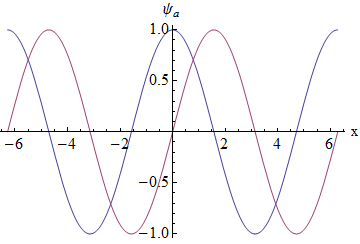
\includegraphics[scale=0.6]{images/oscillitary-psi-a}}
		\caption{$\psi_{a}$}
		\label{}
	\end{subfigure}
	\hspace{1.2cm}
	\begin{subfigure}{0.45\textwidth}
		\centerline{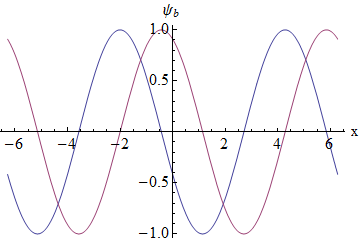
\includegraphics[scale=0.6]{images/oscillitary-psi-b}}
		\caption{$\psi_{b}$}
		\label{}
	\end{subfigure}
	\caption{Example plots of wave-function against spacial direction from Equation (\ref{introduction-wf}). Here oscillatory wave-functions are shown where the blue curves are the real component and the red curves are the imaginary component. The $\psi_{a}$ component of the graphene wave-function is shown in (a) and the $\psi_{b}$ component is shown in (b).}
	\label{oscillitary-psi-a}
\end{figure}
%%%%%
%%%%%
%%%%%
			\subsection{Growth and Decay}
			\label{Wave-functions - Growth and Decay}
				Here wave-functions which display exponential growth and decay are found. These will be useful for calculating bound states. By requiring that $\psi_{a}$ is of the form:
				\begin{align}
					\psi_{a}=\left(a_{1}e^{q_{d}x}+a_{2}e^{-q_{d}x}\right)e^{ik_{y}y}
				\end{align}
				$\psi_{b}$ can be found from the graphene Hamiltonian.
				\begin{align}
					\psi_{b}&=\frac{\hbar v_{f}}{V-E-m}\left(i\frac{\partial}{\partial x}-\frac{\partial}{\partial y}\right)\psi_{a}
				\end{align}
				Evaluating this shows:
				\begin{align}
					\psi_{b}=i\left(a_{1}\alpha_{-}e^{q_{d}x}-a_{2}\alpha_{+}e^{-q_{d}x}\right)e^{ik_{y}y}
				\end{align}
				With the group of constants defined as:
				\begin{align}
					\alpha_{\pm}=\frac{\hbar v_{f}}{V-E-m}\left(q_{d}\pm k_{y}\right)
				\end{align}
				The wave-functions should then be inserted into the Dirac equation to check validity.
				\begin{align}
					\hat{H}\psi=E\psi
				\end{align}
				\begin{align}
					\left[\begin{array}{ccc}
						V-E+m&-\hbar v_{f}\left(i\frac{\partial}{\partial x}+\frac{\partial}{\partial y}\right)\\
						-\hbar v_{f}\left(i\frac{\partial}{\partial x}-\frac{\partial}{\partial y}\right)&V-E-m
					\end{array}\right]
					\left[\begin{array}{ccc}
						a_{1}e^{q_{d}x}+a_{2}e^{-q_{d}x}\\
						i\left(\alpha_{-}a_{1}e^{q_{d}x}-\alpha_{+}a_{2}e^{-q_{d}x}\right)
					\end{array}\right]e^{ik_{y}y}
					=0
				\end{align}
				This provides the two equations:
				\begin{align}
					\left(V-E+m\right)\left(a_{1}e^{q_{d}x}\right. &+ \left.a_{2}e^{-q_{d}x}\right)e^{ik_{y}y}\\
					&-\hbar v_{f}\left(i\frac{\partial}{\partial x}+\frac{\partial}{\partial y}\right)\left(\alpha_{-}a_{1}e^{q_{d}x}-\alpha_{+}a_{2}e^{-q_{d}x}\right)e^{ik_{y}y}=0
				\end{align}
				\begin{align}
					-\hbar v_{f}\left(i\frac{\partial}{\partial x}-\frac{\partial}{\partial y}\right)\left(a_{1}e^{q_{d}x}\right. &+ \left. a_{2}e^{-q_{d}x}\right)e^{ik_{y}y}\\
					&+i\left(V-E-m\right)\left(\alpha_{-}a_{1}e^{q_{d}x}-\alpha_{+}a_{2}e^{-q_{d}x}\right)e^{ik_{y}y}=0
				\end{align}
				Which show that:
				\begin{align}
					q_{d}=\sqrt{k_{y}^{2}-\frac{\left(E-V\right)^{2}+m^{2}}{\hbar^{2}v_{f}^{2}}}
				\end{align}
				With this value of $q_{d}$ the wave-functions satisfy the Dirac equation so the wave-functions can finally take the form:
				\begin{align}
					\psi=e^{ik_{y}y}
					\left[\begin{array}{ccc}
						e^{q_{d}x}&e^{-q_{d}x}\\
						i\alpha_{-}e^{q_{d}x}&-i\alpha_{+}e^{-q_{d}x}
					\end{array}\right]
					\left[\begin{array}{ccc}
						a_{1}\\
						a_{2}
					\end{array}\right]
					\label{introduction-wf-gd}
				\end{align}
				With $m=0$ these wave-functions match the wave-functions in \cite{b3}. The exponential growth wave-functions have been plotted in Figure \ref{growth-psi-a}. This plot shows that both the $\psi_{a}$ and $\psi_{b}$ terms are exponentially growing with real only components in $\psi_{a}$ and imaginary only components in $\psi_{b}$. As with the oscillatory case the $\psi_{b}$ component experiences a phase shift.
\begin{figure}
	\begin{subfigure}{0.45\textwidth}
		\centerline{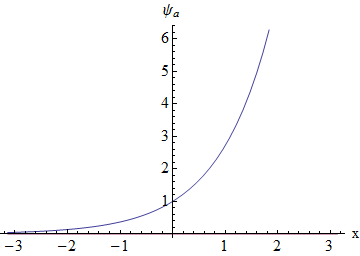
\includegraphics[scale=0.6]{images/growth-psi-a}}
		\caption{$\psi_{a}$}
		\label{}
	\end{subfigure}
	\hspace{1.2cm}
	\begin{subfigure}{0.45\textwidth}
		\centerline{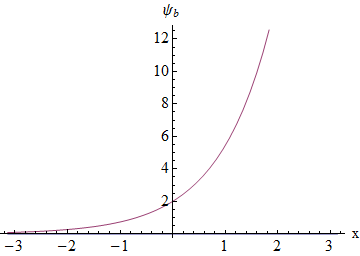
\includegraphics[scale=0.6]{images/growth-psi-b}}
		\caption{$\psi_{b}$}
		\label{}
	\end{subfigure}
	\caption{Example plots of wave-function against spacial direction from Equation (\ref{introduction-wf-gd}). Here exponential growth wave-functions are shown where the blue curves are the real component and the red curves are the imaginary component. The $\psi_{a}$ component of the graphene wave-function is shown in (a) and the $\psi_{b}$ component is shown in (b).}
	\label{growth-psi-a}
\end{figure}
%%%%%
%%%%%
%%%%%
	\section{Magnetic Field}
		\label{Introduction - Magnetic Field}
		In this section the properties of infinite sheet graphene will be examined with an external perpendicular magnetic field applied to it. The momentum must be modified to account for the contributions from the magnetic field by the Peierls substitution \cite{b39}. In a magnetic field the linear energy-momentum relation will be replaced by energy levels. These energy levels will be obtained using the modified graphene Hamiltonian for magnetic field. Finally this Hamiltonian will be used to obtain wave-functions for charge carriers in an infinite sheet of graphene with an external magnetic field.
		\subsection{Peierls Substitution}
			The Peierls substitution changes the expression for momentum to allow for an external magnetic field. To do this a charged particle of charge $q$ can be considered. When a charged particle moves though a magnetic field, the Lorentz force associated with this particle is:
			\begin{equation}
				\vec{F}=q\left(\vec{E}+\vec{v}\times \vec{B}\right)
			\end{equation}
			Where the electric and magnetic field strengths are defined as:
			\begin{align}
			\vec{B}=\bigtriangledown \times \vec{A}\hspace{1cm}\vec{E}=-\bigtriangledown\phi-\frac{d\vec{A}}{dt}
			\end{align}
			Substituting these definitions into the Lorentz force provides:
			\begin{equation}
				\vec{F}=q\left(-\bigtriangledown\phi-\frac{d\vec{A}}{dt}+\bigtriangledown\left(\vec{v}\cdot\vec{A}\right)\right)
			\end{equation}
			The force is related to potential energy by:
			\begin{align}
				\vec{F}=-\bigtriangledown V\left(\vec{r}\right)\hspace{1cm}V\left(\vec{r}\right)=-\int\vec{F}d\vec{r}
			\end{align}
			Converting the force into a potential and with the condition $d\vec{A}/dt=0$ for a conservative field, results in the potential:
			\begin{equation}
				V\left(\vec{r}\right)=q\left(\phi-\vec{v}\cdot\vec{A}\right)
				\label{peierl-v}
			\end{equation}
			The Lagrangian is defined as:
			\begin{equation}
				L=T-V
			\end{equation}
			Where $T$ is the kinetic energy and $V$ is the potential energy. With the general definition of kinetic energy and potential energy from Equation (\ref{peierl-v}):
			\begin{equation}
				L=\frac{1}{2}m\vec{v}^{2}-q\phi+\frac{q}{c}\vec{v}\cdot\vec{A}
				\label{peierl-L}
			\end{equation}
			To find the momentum from the Lagrangian:
			\begin{equation}
				\frac{dL}{d\vec{v}}=\vec{p}=m\vec{v}+q\vec{A}
				\label{lagrangian momentum}
			\end{equation}
			Using definitions of the Hamiltonian and Lagrangian, the Hamiltonian can be obtained form the Langrangian with the relation:
			\begin{equation}
				H=T+V=2T-L=\vec{v}\cdot\vec{p}-L
			\end{equation}
			With the definition of the Lagrangian from Equation (\ref{peierl-L}):
			\begin{align}
				H&=\vec{v}\cdot\left(m\vec{v}+q\vec{A}\right)-\frac{1}{2}m\vec{v}^{2}+q\phi-q\vec{v}\cdot\vec{A}\\
				&=\frac{1}{2}m\vec{v}^{2}+q\phi
			\end{align}
			The velocity can be expressed as momentum from Equation (\ref{lagrangian momentum}):
			\begin{equation}
				\vec{v}=\frac{1}{m}\left(\vec{p}-q\vec{A}\right)
			\end{equation}
			Resulting in the Hamiltonian:
			\begin{equation}
				H=\frac{1}{2m}\left(\vec{p}-q\vec{A}\right)^{2}+q\phi
			\end{equation}
			The Peierls substitution for momentum in a magnetic field becomes \cite{b39}:
			\begin{equation}
				\vec{p}\rightarrow \vec{p}-q\vec{A}
			\end{equation}
			This substitution for momentum in a magnetic field may also be refered to as canonical momentum.
%%%%%
%%%%%
%%%%%
		\subsection{Landau Levels}
			Under a magnetic field the linear energy-momentum relation is replaced by energy levels \cite{b33}. The Landau levels for graphene in a magnetic field can be derived by using Peierls substitution. The uniform magnetic field is introduced in the $z$ direction.
			\begin{align}
				\hat{H}=v_{f}\sigma \hat{p}
				\hspace{1cm}
				\hat{p}\rightarrow \hat{p}+e\vec{A}
				\hspace{1cm}
				l_{b}=\sqrt{\frac{\hbar}{eB_{0}}}
				\hspace{1cm}
				\vec{B}=
				\left[\begin{array}{ccc}
					0\\
					0\\
					B_{0}
				\end{array}\right]
				\hspace{1cm}
				\vec{A}=B_{0}
				\left[\begin{array}{ccc}
					0\\
					x\\
					0
				\end{array}\right]
			\end{align}
			Using the secular equation $\det\left(\hat{H}-E\right)=0$ produces:
			\begin{equation}
				\frac{E^{2}}{v_{f}^{2}}-\left(\hat{p}_{x}+i\hat{p}_{y}+\frac{i\hbar x}{ l_{b}^{2}}\right)\left(\hat{p}_{x}-i\hat{p}_{y}-\frac{i\hbar x}{ l_{b}^{2}}\right)=0
			\end{equation}
			With the commutation relations:
			\begin{equation}
				\left[\hat{p}_{x},\hat{p}_{y}\right]=0\hspace{1cm}\left[\hat{p}_{x},\hat{x}\right]=-i\hbar
			\end{equation}
			This equation can act on a wave-function with the form $\psi_{a}=f(x)e^{ik_{y}y}$ to replace the $y$ momentum with the corresponding eigenvalue. The equation:
			\begin{equation}
				\left[\frac{E^{2}}{v_{f}^{2}}-\left(\hat{p}_{x}+i\hat{p}_{y}+\frac{i\hbar x}{ l_{b}^{2}}\right)\left(\hat{p}_{x}-i\hat{p}_{y}-\frac{i\hbar x}{ l_{b}^{2}}\right)\right]\psi_{a}=0
			\end{equation}
			can be reduced to:
			\begin{equation}
				\frac{l_{b}^{2}}{\hbar^{2}v_{f}^{2}}E^{2}+1-\frac{l_{b}^{2}}{\hbar^{2}}\hat{p}_{x}^{2}-\frac{1}{l_{b}^{2}}\left(x+l_{b}^{2}k_{y}\right)^{2}=0
				\label{introduction-mag-int}
			\end{equation}
			With the additional substitutions:
			\begin{equation}
				\varepsilon=E^{2}+\frac{\hbar^{2}v_{f}^{2}}{l_{b}^{2}}\hspace{1cm}{\bar x}=x+l_{b}^{2}k_{y}
			\end{equation}
			Equation (\ref{introduction-mag-int}) can be written as:
			\begin{equation}
				\frac{l_{b}^{2}}{\hbar^{2}v_{f}^{2}}\varepsilon-\frac{l_{b}^{2}}{\hbar^{2}}\hat{p}_{x}^{2}-\frac{1}{l_{b}^{2}}{\bar x}^{2}=0
			\end{equation}
			Which can be matched to the quantum harmonic oscillator derived in Section \ref{Appendix - Quantum Harmonic Oscillator}:
			\begin{equation}
				2mE-\hat{p}_{x}^{2}-m^{2}\omega^{2}x^{2}=0
			\end{equation}
			Then by analogy:
			\begin{equation}
				2m=\frac{l_{b}^{2}}{\hbar^{2}v_{f}^{2}}\hspace{1cm}1=\frac{\hbar^{2}}{l_{b}^{2}}\hspace{1cm}m^{2}\omega^{2}=\frac{1}{l_{b}^{2}}\hspace{1cm}\omega=2\frac{\hbar v_{f}^{2}}{l_{b}^{2}}
			\end{equation}
			The known result for the quantum harmonic oscillator $E_{n}=\hbar\omega\left(n+1/2\right)$ can be converted to the graphene case, resulting in \cite{b37, b53}:
			\begin{equation}
				E_{n}=\pm \frac{\hbar v_{f}}{l_{b}}\sqrt{2n}
				\label{landau-levels-e}
			\end{equation}
			If an external potential and constant energy gap are introduced into the graphene Hamiltonian the Landau levels change to:
			\begin{equation}
				E_{n}=V \pm \frac{\hbar v_{f}}{l_{b}}\sqrt{\frac{l_{b}^{2}}{\hbar^{2}v_{f}^{2}}m^{2}+2n}
				\label{landau-levels-e-m}
			\end{equation}

			In Figure \ref{landau-levels} the first five Landau levels are shown with their dependencies on the magnetic length $l_{b}$. In Figure \ref{landau-levels} (b) an energy gap and external potential have been included. The energy gap increase the gap between the first energy level, which in turn causes the energy levels to be found closer to eachother. The external potential shifts the levels in the energy axis.
			\begin{figure}
				\begin{subfigure}{0.45\textwidth}
					\centerline{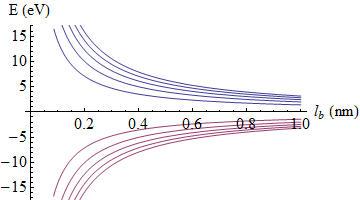
\includegraphics[scale=0.6]{images/landau-levels}}
					\caption{$V=0$ eV and $m=0$ eV.}
				\end{subfigure}
				\hspace{1.2cm}
				\begin{subfigure}{0.45\textwidth}
					\centerline{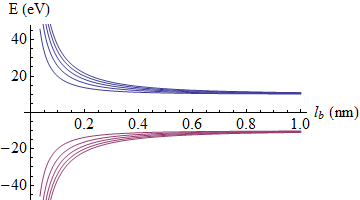
\includegraphics[scale=0.6]{images/landau-levels-v-m}}
					\caption{$V=5$ eV and $m=5$ eV.}
				\end{subfigure}
				\caption{Plot showing the first five Landau levels and their dependence on magnetic length $l_{b}$ from Equation (\ref{landau-levels-e}) and Equation (\ref{landau-levels-e-m}). Here $\hbar v_{f}$ has been taken to be equal to one.}
				\label{landau-levels}
			\end{figure}

%%%%%
%%%%%
%%%%%
			\subsection{Wave-functions}
			\label{Wave-functions - Magnetic Field}
				The wave-functions for graphene in a magnetic field can be derived from the graphene Hamiltonian with Peierls substitution.
				\begin{align}
					\hat{H}=v_{f}\sigma \hat{p}+IV+\sigma_{z}m\hspace{1cm}\hat{p}\rightarrow \hat{p}+e\vec{A}
				\end{align}
				With an external magnetic field in the $z$ direction and the Landau gauge:
				\begin{align}
					l_{b}=\sqrt{\frac{\hbar}{eB_{0}}}
					\hspace{1cm}\vec{B}=
					\left[\begin{array}{ccc}
						0\\
						0\\	
						B_{0}
					\end{array}\right]
					\hspace{1cm}\vec{A}=B_{0}
					\left[\begin{array}{ccc}
						0\\
						x\\
						0
					\end{array}\right]
					\hspace{1cm}I=\left[\begin{array}{ccc}
						1 & 0\\
						0 & 1
					\end{array}\right]
				\end{align}
				The time independent Dirac equation becomes:
				\begin{align}
					\left[\begin{array}{ccc}
						V-E+m&v_{f}\left(\hat{p}_{x}-i\hat{p}_{y}-i\frac{\hbar}{l_{b}^{2}}x\right)\\
						v_{f}\left(\hat{p}_{x}+i\hat{p}_{y}+i\frac{\hbar}{l_{b}^{2}}x\right)&V-E-m
					\end{array}\right]
					\left[\begin{array}{ccc}
						\psi_{a}\\
						\psi_{b}
					\end{array}\right]=0
				\end{align}
				Expressing this as simultaneous equations:
				\begin{align}
					\left(V-E+m\right)\psi_{a}+v_{f}\left(\hat{p}_{x}-i\hat{p}_{y}+i\frac{\hbar}{l_{b}^{2}}x\right)\psi_{b}=0\\
					v_{f}\left(\hat{p}_{x}+i\hat{p}_{y}-i\frac{\hbar}{l_{b}^{2}}x\right)\psi_{a}+\left(V-E-m\right)\psi_{b}=0
				\end{align}
				Then $\psi_{b}$ can be removed  by the relation:
				\begin{align}\label{eq:spinor}
					\psi_{b}=\frac{v_{f}\left(\hat{p}_{x}+i\hat{p}_{y}-i\frac{\hbar}{l_{b}^{2}}x\right)}{E-V+m}\psi_{a}
				\end{align}
				The commutator $[\hat{p}_{x},\hat{x}]$ produces:
				\begin{align}
					\frac{m^{2}-\left(E-V\right)^{2}}{v_{f}^{2}}\psi_{a}+\left(\hat{p}_{x}^{2}-\frac{\hbar^2}{l_{b}^{2}}+\hat{p}_{y}^{2}-2\frac{\hbar}{l_{b}^{2}}\hat{p}_{y}x+\frac{\hbar^{2}}{l_{b}^{4}}x^{2}\right)\psi_{a}=0
				\end{align}
				To provide plane waves in the $y$ direction, separable solutions in the form of $\psi_{a}=f(x)e^{ik_{y}y}$ are required. Evaluting this provides the ODE:
				\begin{align}
					-f''(x)+\left(\frac{1}{\hbar^{2} v_{f}^{2}}\varepsilon+\frac{1}{l_{b}^{4}}\left(x-l_{b}^{2}k_{y}\right)^{2}\right)f(x)=0
					\label{magnetic-ode}
				\end{align}
				Where constants have been grouped and the change in variables will be introduced:
				\begin{align}
					\varepsilon=\left(E-V\right)^{2}-m^{2}+\frac{\hbar^2 v_{f}^{2}}{l_{b}^{2}}\hspace{1cm}{\bar x}=x-l_{b}^{2} k_{y}
				\end{align}
				With the change in variables Equation (\ref{magnetic-ode}) has the solution:
				\begin{align}
					f(x)=c_{1}D_{-\frac{1}{2}\left(\frac{l_{b}^{2}\varepsilon}{\hbar^2 v_{f}^{2}}+1\right)}\left(\sqrt{2}l_{b}{\bar x}\right)+c_{2}D_{\frac{1}{2}\left(\frac{l_{b}^{2}\varepsilon}{\hbar^2 v_{f}^{2}}-1\right)}\left(i\sqrt{2}l_{b}{\bar x}\right)
				\end{align}
				Where $D_{n}\left(x\right)$ is the parabolic cylinder function. With the following substitution:
				\begin{align}
					\Delta=\frac{1}{2}\frac{l_{b}^{2}\varepsilon}{\hbar^2 v_{f}^{2}}
				\end{align}
				This can be simplified to:
				\begin{align}
					\psi_{a}=c_{1}D_{-\Delta-\frac{1}{2}}\left(\sqrt{2}l_{b}{\bar x}\right)+c_{2}D_{\Delta-\frac{1}{2}}\left(i\sqrt{2}l_{b}{\bar x}\right)
					\label{introduction-mag-a}
				\end{align}
				To find the wave-function component $\psi_{b}$, the result for $\psi_{a}$ can be inserted into Equation (\ref{eq:spinor}) to provide:
				\begin{align}
					\psi_{b}&=\frac{i\hbar v_{f}}{E-V+m}\left(c_{1}\left(\frac{\sqrt{2}}{l_{b}}D_{\Delta+\frac{1}{2}}\left(\sqrt{2}l_{b}{\bar x}\right)+2\frac{{\bar x}}{\hbar}D_{\Delta-\frac{1}{2}}\left(\sqrt{2}l_{b}{\bar x}\right)\right)\right.\\
					&+\left.c_{2}\left(i\frac{\sqrt{2}}{l_{b}}D_{-\Delta+\frac{3}{2}}\left(i\sqrt{2}l_{b}{\bar x}\right)-2\frac{{\bar x}}{\hbar}D_{-\Delta+\frac{1}{2}}\left(i\sqrt{2}l_{b}{\bar x}\right)\right)\right)
					\label{introduction-mag-b}
				\end{align}
				The reflected component can then be included by replacing $\bar{x}$ with $-\bar{x}$. Due to these substitutions the oscillatory wave-functions must also be switched to the new axis. The oscillatory wave-functions become:
				\begin{equation}
					\psi=
					\left[\begin{array}{ccc}
						e^{iq\left({\bar x}+l_{b}^{2}k_{y}\right)}\\
						\alpha_{1}e^{iq\left({\bar x}+l_{b}^{2}k_{y}\right)+i\theta}
					\end{array}\right]
				\end{equation}
				The magnetic field wave-functions have been plotted in Figure \ref{magnetic-psi-a}. This plot shows the real and imaginary components of each component of the wave-function. As these wave-functions tend to infinities as ${\bar x}$ increases it is reasonable to remove a specific component of the wave-function on physical grounds depending on the problem.
\begin{figure}
	\begin{subfigure}{0.45\textwidth}
		\centerline{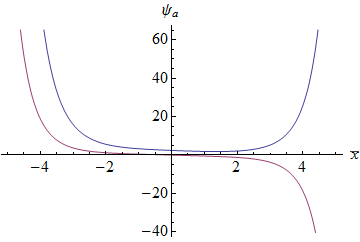
\includegraphics[scale=0.6]{images/magnetic-psi-a}}
		\caption{$\psi_{a}$}
		\label{}
	\end{subfigure}
	\hspace{1.2cm}
	\begin{subfigure}{0.45\textwidth}
		\centerline{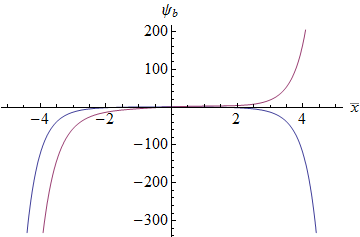
\includegraphics[scale=0.6]{images/magnetic-psi-b}}
		\caption{$\psi_{b}$}
		\label{Magenetic Field wave-functions}
	\end{subfigure}
	\caption{Example plots of wave-function against spacial direction from Equation (\ref{introduction-mag-a}) and Equation (\ref{introduction-mag-b}). Here the wave-functions are shown where the blue curves are the real component and the red curves are the imaginary component. The $\psi_{a}$ component of the graphene wave-function is shown in (a) and the $\psi_{b}$ component is shown in (b).}
	\label{magnetic-psi-a}
\end{figure}
%%%%%
%%%%%
%%%%%
%%%%%
%%%%%
		\section{Density of States}
		\label{Introduction - Density of States}
			The density of states calculation will show the number of available energy states for charge carriers at each energy. Using the linear spectrum of graphene, this calculation can be adapted for the graphene case. The general form of density of states \cite{b3}:
			\begin{equation}
				\rho\left(E\right)=\sum_{k}\delta\left(E-E_{k}\right)
			\end{equation}
			Converting sum notation to integration in two dimensions, the density of states becomes:
			\begin{equation}
				\rho\left(E\right)=\frac{L_{x}L_{y}}{4\pi^{2}}2\int_{k}\int_{\theta}\delta\left(E-E_{k}\right)kdkd\theta
			\end{equation}
			where $L_{x,y}$ is the size of the graphene sheet in the respective direction with 2 spin degeneracy. From the linear spectrum of graphene the relations:
			\begin{align}
				E_{k}=\hbar v_{f}k
				\hspace{1cm}
				dE_{k}=\hbar v_{f}dk
				\hspace{1cm}
				kdk=\frac{E_{k}}{\hbar^{2}v_{f}^{2}}dE_{k}
			\end{align}
			can be made and the density of states becomes:
			\begin{equation}
				\rho\left(E\right)=\frac{L_{x}L_{y}}{2\pi^{2}}\int_{-\infty}^{\infty}\delta\left(E-E_{k}\right)2\pi \frac{E_{k}}{\hbar^{2}v_{f}^{2}}dE_{k}
			\end{equation}
			Using the Dirac delta function rule and 2 valley degeneracy for electrons and holes, the graphene density of states for a linear spectrum becomes \cite{b3}:
			\begin{equation}
				\rho\left(E\right)=\frac{2L_{x}L_{y}}{\pi\hbar^{2}v_{f}^{2}}|E|
				\label{introduction-dos}
			\end{equation}
			If instead of the linear energy spectrum, the graphene spectrum with an energy gap may be used the following adaptations:
			\begin{align}
				E_{k}=\sqrt{\hbar^{2} v_{f}^{2}\left(k_{x}^{2}+k_{y}^{2}\right)+m^{2}}
				\hspace{1cm}
				k=\frac{\sqrt{E_{k}^{2}-m^{2}}}{\hbar v_{f}}
				\hspace{1cm}
				kdk=\frac{E_{k}}{\hbar^{2}v_{f}^{2}}dE_{k}
			\end{align}
			Resulting in the same equation for the linear density of states in graphene.
%%%%%
%%%%%
%%%%%
		\section{Landauer Formalism}
		\label{Introduction - Landauer Formalism}
			It will be useful to determine the current through a graphene nano-device. For a single channel system at non-zero temperatures the current  through the system shown in Figure \ref{introduction-current} can be found \cite{b6}.
			\begin{figure}[h]
				\centerline{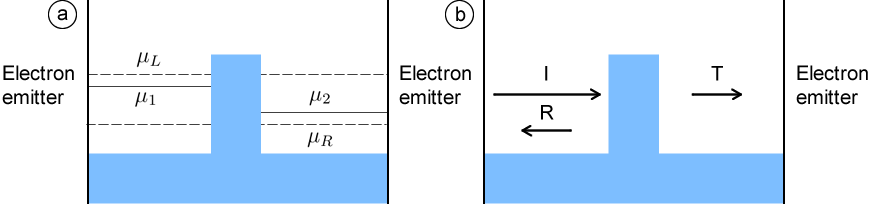
\includegraphics[scale=0.5]{images/current}}
				\caption{(a) Diagram showing quasi-Fermi-energies and chemical potentials of the perfectly conducting wires. Here the left emitter injects electrons up to the quasi-Fermi-energy $\mu_{L}$ and the right emitter injects electrons up the the quasi-Fermi-energy $\mu_{R}$. $\mu_{1}$ and $\mu_{2}$ are the chemical potentials of the perfectly conducting wires to the left and right of the scattering device. (b) A scattering device between two electron emitters. Charge carriers from the left emitter are scattered with a probability $R$ of being reflected and probability $T$ of transmitting through the scattering device.}
				\label{introduction-current}
			\end{figure}
			 The system in Figure \ref{introduction-current} consists of two incoherent electron reservoirs, which emit charge carriers up to the quasi-Fermi-energy $\mu_{L,R}$, where the subscript $L$ and $R$ represent the reservoir at each side of the system. These reservoirs are then connected to a scattering device via perfect and identical one dimensional conductors. These conductors have chemical potentials $\mu_{1}$ and $\mu_{2}$. The current from the left reservoir to the right is then:
			\begin{equation}
				I=ev\frac{dn}{dE}\left(\mu_{L}-\mu_{R}\right)
				\label{current-dos}
			\end{equation}
			The current that is transmitted through the sample is:
			\begin{equation}
				I=\frac{e}{\pi\hbar}T\left(\mu_{L}-\mu_{R}\right)
				\label{current-transmit}
			\end{equation}
			Where the one dimensional density of states $dn/dE=1/\hbar\pi v$. The total number of states in each conducting wire is given by the density of states and the energy range available; $2\left(dn/dE\right)\left(\mu_{L}-\mu_{R}\right)$. On the right side the number of occupied states is therefore $T\left(dn/dE\right)\left(\mu_{L}-\mu_{2}\right)$ and the unoccupied states is then $\left(2-T\right)\left(dn/dE\right)\left(\mu_{2}-\mu_{R}\right)$. The chemical potential of the right wire can then be determined by:
			\begin{equation}
				T\left(dn/dE\right)\left(\mu_{L}-\mu_{2}\right)=\left(2-T\right)\left(dn/dE\right)\left(\mu_{2}-\mu_{R}\right)
				\label{mu-a}
			\end{equation}
			The left wire contains the incident electrons as well as any reflected electrons. The occupied states is then $\left(1+R\right)\left(dn/dE\right)\left(\mu_{L}-\mu_{1}\right)$ and the unoccupied states $\left(2-\left(1+R\right)\right)$ $\left(dn/dE\right)\left(\mu_{1}-\mu_{R}\right)$. An expression for $\mu_{1}$ can then be found:
			\begin{equation}
				\left(1+R\right)\left(dn/dE\right)\left(\mu_{L}-\mu_{1}\right)=\left(2-\left(1+R\right)\right)\left(dn/dE\right)\left(\mu_{1}-\mu_{R}\right)
				\label{mu-b}
			\end{equation}
			The difference in the bottoms of the conduction bands can then be represented by the potential difference:
			\begin{equation}
				eV=\mu_{1}-\mu_{2}
			\end{equation}
			With Equation (\ref{mu-a}) and Equation (\ref{mu-b}) this potential can be represented by $eV=R\left(\mu_{L}-\mu_{R}\right)$. Then with the definition of conductance, this potential difference and Equation (\ref{current-transmit}) the conductance can be expressed as:
			\begin{equation}
				G=\frac{I}{V}=\frac{e^{2}}{\pi\hbar}\frac{T}{R}
				\label{GTR}
			\end{equation}
			At non-zero temperatures the reservoirs do not fully fill the states up to the quasi-Fermi-energies, instead they are filled according to the Fermi-Dirac distributions:
			\begin{equation}
				f\left(E-\mu_{L,R}\right)=\frac{1}{e^{\frac{E-\mu_{L,R}}{k_{b}t}}+1}
			\end{equation}
			where $k_{b}$ is the Boltzmann constant and $t$ is the temperature. With these distributions the quasi-Fermi-energies can be replaced. Then by integrating with respect to energy the current in Equation (\ref{current-transmit}) becomes:
			\begin{equation}
				I=\frac{e}{\pi\hbar}\int T\left[f\left(E-\mu_{L}\right)-f\left(E-\mu_{R}\right)\right] dE
				\label{current-temp}
			\end{equation}
			To find the conductance at non-zero temperatures the chemical potentials in Equation (\ref{mu-a}) and Equation (\ref{mu-b}) must be multiplied by the Fermi distributions and integrated.
			\begin{equation}
				\mu_{1}=\frac{\int\left(\frac{-df}{dE}\frac{dn}{dE}R\left(E\right)\left(\mu_{L}-\mu_{R}\right)+\mu_{L}\right)dE}{\int\frac{-df}{dE}\frac{dn}{dE}dE}
				\hspace{1cm}
				\mu_{2}=\frac{\int\left(\frac{-df}{dE}\frac{dn}{dE}T\left(E\right)\left(\mu_{L}-\mu_{R}\right)+\mu_{R}\right)dE}{\int\frac{-df}{dE}\frac{dn}{dE}dE}
			\end{equation}
 			Where the definition:
			\begin{equation}
				\frac{-df}{dE}=\left[f\left(E-\mu_{L}\right)-f\left(E-\mu_{R}\right)\right]/\left(\mu_{L}-\mu_{R}\right)
			\end{equation}
			will be used. Assuming the velocity has a negligible dependence on energy, the voltage at finite temperature is now:
			\begin{equation}
				eV=\frac{\int \frac{-df}{dE}R\left(E\right) \left(dn/dE\right)dE}{\int \frac{-df}{dE}\left(dn/dE\right)dE}\left(\mu_{L}-\mu_{R}\right)
				\label{voltage-temp}
			\end{equation}
			With Equation (\ref{current-temp}) and Equation (\ref{voltage-temp}) the conductance at non-zero temperatures is:
			\begin{equation}
				G=\frac{e^{2}}{\pi\hbar}\int T\left(E\right)\frac{-df}{dE} dE \frac{\int \frac{-df}{dE}\left(dn/dE\right)dE}{\int \frac{-df}{dE}R\left(E\right) \left(dn/dE\right)dE}
				\label{conductance-temperature}
			\end{equation}
			At zero temperature and with small voltages across the source-drain $\frac{-df}{dE}$ becomes $\delta \left(E-E_{f}\right)$, the integrals are removed by the identity $\int f(x)\delta(x) dx=f(0)$ and Equation (\ref{conductance-temperature}) reduces to Equation (\ref{GTR}). In the case of $R=0$ this result produces infinite conductance. However, \cite{b7} shows that for any length of perfect conductor an electric field can be absorbed and the condition of $R\approx 1$ can be used. For a system with a region of perfect transmission the conductance is given to be:
			\begin{equation}
				G=\frac{e^{2}}{\pi\hbar}T\left(\mu_{L}-\mu_{R}\right)
			\end{equation}
			Therefore the result at non-zero temperatures, with a region of perfect transmission becomes:
			\begin{equation}
				G=\frac{e^{2}}{\pi\hbar}\int T\left[f\left(E-\mu_{L}\right)-f\left(E-\mu_{R}\right)\right]dE
			\end{equation}
%%%%%
%%%%%
%%%%%
		\section{Landauer Formalism in Graphene}
		\label{Introduction - Landauer Formalism in Graphene}
			In this section the Landauer formalism is derived for a graphene scattering device. For a single channel system at non-zero temperatures the current through the system shown in Figure \ref{introduction-current} can be found \cite{b6}.
			 The system in Figure \ref{introduction-current} consists of 2 incoherent electron reservoirs, which emit charge carriers up to the quasi-Fermi-energy $\mu_{L,R}$, where the subscript $L$ and $R$ represent the reservoir at left or right side of the system respectivly. These reservoirs are then connected to a scattering device via perfect and identical one dimensional conductors. These conductors have chemical potentials $\mu_{1}$ and $\mu_{2}$. The current from the left reservoir to the right is then:
			\begin{equation}
				I=ev_{f}\frac{dn}{dE}\left(\mu_{L}-\mu_{R}\right)
				\label{current-dos}
			\end{equation}
			Where $e$ is the electron charge, $v_{f}$ is the Fermi velocity and $dn/dE$ is the density of states. The current that is transmitted through the sample is then:
			\begin{equation}
				I=ev_{f}\frac{dn}{dE}T\left(\mu_{L}-\mu_{R}\right)
				\label{current-transmit-graphene}
			\end{equation}
			Where $T$ is the transmission probability through the scattering device. In \cite{b1} the density of states for a single unit cell of graphene at a Dirac point is given by:
			\begin{equation}
				\frac{dn}{dE}=\frac{2A_{c}}{\pi}\frac{|E|}{\hbar^{2}v_{f}^{2}}
				\hspace{1cm}
				A_{c}=\frac{3\sqrt{3}a^{2}}{2}
			\end{equation}
			The definition $L_{x}L_{y}/A_{c}$ is the number of unit cells in the sample, where  $L_{x}, L_{y}$ is the size of the sample in the respective dimension and $A_{c}$ is the area of the graphene unit cell. As only the $x$ direction current will be considered here, the current in the $x$ direction will be the same in each cell, therefore only the number of graphene unit cells in the $y$ direction will affect the $x$ directional current. This way the quantity $L_{x}$ can be set to one and removed from the calculation. The current through the graphene sample from Equation (\ref{current-transmit-graphene}) in the $x$ direction becomes:
			\begin{equation}
				I_{x}=e\frac{2L_{y}}{\pi \hbar^{2}v_{f}}T\left(E,\theta\right)\left(\mu_{L}-\mu_{R}\right)|E|\cos(\theta)
			\end{equation}
			The energy $\left(E\right)$ and incident angle $\left(\theta\right)$ dependence for $T$ has been included here to allow for the graphene transmission probability. At non-zero temperatures the states are instead filled according to the corresponding Fermi-Dirac distribution.
			\begin{equation}
				f\left(E-\mu_{L,R}\right)=\frac{1}{e^{\frac{E-\mu_{L,R}}{k_{b}t}}+1}
			\end{equation}
			where $k_{b}$ is the Boltzmann constant and $t$ is the temperature. The current must then be integrated over all energies and values of theta to account for all states in the Fermi-Dirac distributions.
			\begin{equation}
				I_{x}=I_{0}\int^{\infty}_{-\infty}\int^{\pi/2}_{-\pi/2}T\left(E,\theta\right)\left[f\left(E-\mu_{L}\right)-f\left(E-\mu_{R}\right)\right]|E|\cos(\theta)dEd\theta
				\label{introduction-i-graphene}
			\end{equation}
			Here, the group of constants $I_{0}=e\frac{2L_{y}}{\pi\hbar^{2}v_{f}}$ has been introduced. At this stage the current shows a similar form to that in \cite{b9, b10}, with the exception that the graphene density of states causes an additional $|E|$ term and the graphene transmission probability introduces a theta dependence. This result for current can then be used with the definition of conductance $G=I/V$ to find the conductance at a finite temperature for graphene. The potential difference $V$ is determined by the number of charges on the left and right of the scattering device. This can be found by considering the chemical potentials of the perfectly conducing wires. The chemical potentials $\mu_{1,2}$ must be between the quasi-Fermi-energies of the electron emitters $\mu_{L,R}$. The positioning of these chemical potentials requires that the number of occupied states (electrons) above $\mu_{1}$ is equal to the number of unoccupied states (holes) below $\mu_{1}$, and likewise for states above and below $\mu_{2}$. As all states below $\mu_{R}$ must be filled, only the energy range between $\mu_{L}$ and $\mu_{R}$ needs to be considered. Allowing for positive and negative velocities the number of states between this range is $2\left(dn/dE\right)\left(\mu_{L}-\mu_{R}\right)$. To the right of the scattering device the number of occupied states is the total number of states available in the wire multiplied by the transmission probability; $T\left(dn/dE\right)\left(\mu_{L}-\mu_{2}\right)$. The number of unoccupied states must therefore be the total number of states available in the wire minus the filled states $\left(2-T\right)\left(dn/dE\right)\left(\mu_{2}-\mu_{R}\right)$. As the number of occupied states is equal to the number of unoccupied states we can write:
			\begin{equation}
				T\left(dn/dE\right)\left(\mu_{L}-\mu_{2}\right)=\left(2-T\right)\left(dn/dE\right)\left(\mu_{2}-\mu_{R}\right)
				\label{mu-2}
			\end{equation}
			On the left of the scattering device the number of occupied states includes those filled by incident and reflected charge carriers $\left(1+R\right)\left(dn/dE\right)\left(\mu_{L}-\mu_{1}\right)$. The number of unoccupied states is then $\left(2-\left(1+R\right)\right)\left(dn/dE\right)\left(\mu_{1}-\mu_{R}\right)$. The number of occupied and unoccupied states must be equal, therefore:
			\begin{equation}
				\left(1+R\right)\left(dn/dE\right)\left(\mu_{L}-\mu_{1}\right)=\left(2-\left(1+R\right)\right)\left(dn/dE\right)\left(\mu_{1}-\mu_{R}\right)
				\label{mu-1}
			\end{equation}
			The potential difference between the two wires caused by the scattering device is then:
			\begin{equation}
				eV=\mu_{1}-\mu_{2}
			\end{equation}
			Using Equation (\ref{mu-2}) and Equation (\ref{mu-1}) the potential difference across the sample is then:
			\begin{equation}
				eV=R\left(\mu_{L}-\mu_{R}\right)
			\end{equation}
			However, at non-zero temperatures the electron emitters fill the states according to the Fermi-Dirac distibutions. To determine the potential difference at non-zero temperatures Equation (\ref{mu-2}) and Equation (\ref{mu-1}) can be multiplied by the available energy range according to the Fermi-Dirac distributions. Here we will define:
			\begin{equation}
				\frac{-df}{dE}=\left[f\left(E-\mu_{L}\right)-f\left(E-\mu_{R}\right)\right]/\left(\mu_{L}-\mu_{R}\right)
			\end{equation}
			and integrate with respect to energy. This produces the potential difference at non-zero temperatures:
			\begin{equation}
				eV=\frac{\int R\left(E,\theta\right) \frac{-df}{dE} \frac{dn}{dE}dE}{\int\frac{-df}{dE} \frac{dn}{dE}dE}\left(\mu_{L}-\mu_{R}\right)
			\end{equation}
			Using this expression for the voltage and the definition of conductance $G=I/V$ the conductance through a scattering device in graphene can be written as:
			\begin{align}
				G_{x}=e^{2}\frac{2L_{y}}{\pi\hbar^{2}v_{f}}\int^{\infty}_{-\infty}\int^{\pi/2}_{-\pi/2}&T\left(E,\theta\right)\left[f\left(E-\mu_{L}\right)-f\left(E-\mu_{R}\right)\right]|E|\cos(\theta)dEd\theta\\
				&\times\frac{\int\frac{-df}{dE} \frac{dn}{dE}dE}{\int R\left(E,\theta\right) \frac{-df}{dE} \frac{dn}{dE}dEd\theta}\frac{1}{\left(\mu_{L}-\mu_{R}\right)}
			\end{align}
			However, the transmission probability in graphene will become one under resonance conditions, Klein tunnelling or if $\theta=0$. This will cause the reflection probability $R$ to become zero and the voltage to become zero. To allow for this we can restrict the calculation to a system with perfect transmission. As any electric field can be absorbed by a finite region of perfect conductor \cite{b7}, the reflection probability over the entire system will become one. This effect may also be caused by introducing many scattering devices \cite{b6} such as measurement probes. By restricting the calculation to perfect conductors with many scattering devices, $R \approx 1$ and the one dimensional conductance for graphene systems will reduce to:
			\begin{equation}
				G_{x}=e^{2}\frac{2L_{y}}{\pi\hbar^{2}v_{f}}\int^{\pi/2}_{-\pi/2} \int^{\infty}_{-\infty} T\left(E, \theta\right)\frac{f\left(E-\mu_{L}\right)-f\left(E-\mu_{R}\right)}{\mu_{L}-\mu_{R}}|E|\cos(\theta) dE d\theta
				\label{introduction-g-t}
			\end{equation}
			At zero temperature and for small voltages, the Fermi distributions become the Dirac delta function centered at the Fermi energy $E_{f}$. With the identity $\int f(x)\delta(x) dx=f(0)$ the zero temperature conductance for small voltages and large systems becomes:
			\begin{equation}
				G_{x}= G_{0}\int^{\frac{\pi}{2}}_{-\frac{\pi}{2}} T\left(E_{f},\theta\right)|E_{f}|\cos(\theta)d\theta
				\label{introduction-g-zero}
			\end{equation}
			Where constants have been grouped so that $G_{0}=e^{2}\frac{2L_{y}}{\pi\hbar^{2}v_{f}}$. This result for conductance includes the Fermi energy, as required from the density of states of graphene and the integration of a Dirac delta function. A similar result for conductance is shown in \cite{b11, b14,b15}, however many published expressions \cite{b4, b13, b16} for conductance do not include this term. The inclusion of the Fermi energy causes the conductance to become linear outside of the step, or barrier region, dramatically changing the result obtained.
%\end{document}
	%\documentclass[12pt,a4paper]{report}
%\usepackage[utf8]{inputenc}
%\usepackage{amsmath}
%\usepackage{amsfonts}
%\usepackage{amssymb}
%\usepackage[margin=2.5cm]{geometry}
%\usepackage{graphicx}
%\usepackage{caption}
%\usepackage{subcaption}
%\usepackage[nottoc,numbib]{tocbibind}
%\linespread{1.3}

%\DeclareMathOperator\sgn{sgn}

%\begin{document}
	\chapter{The Potential Step}
	\label{Potential Step}
		\begin{figure}
			\centerline{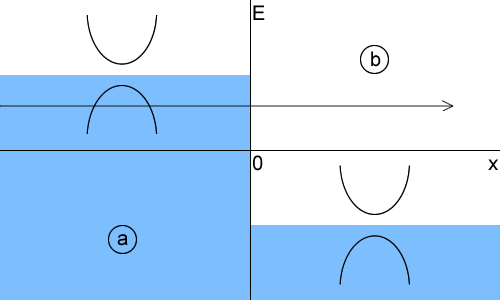
\includegraphics[scale=0.6]{images/rectangular-step-flat}}
			\caption{The graphene potential step centered at $x=0$ with potentials $|V_{a}|=|V_{b}|$ and energy gaps $m_{a,b}$ in the respective region. The parabolic dispersion relation of graphene with an energy gap has been included in each region. This case shows the possibility of Zener tunnelling as a right travelling hole becomes a left travelling electron.}
			\label{rectangular-step-flat}
		\end{figure}
		The potential step is the simplest scattering device with just two wave-function regions \cite{b13} labelled in Figure \ref{rectangular-step-flat} as $a$ and $b$, with potentials $V_{a,b}$ and energy gaps $m_{a,b}$ respectively. As well as two wave-function regions, this problem has three clear energy regions located at $E>V_{a,b}$, $|E|<|V_{a,b}|$ and $E<-V_{a,b}$. Within these regions there is pure electron transport, electron-hole transport and hole-hole transport respectively. When an energy gap is included a fourth energy region must be introduced at $E<V_{a,b}\pm m_{a,b}$ where no transport can occur. This two region problem represents a semiconductor diode and can be used to model Zener tunnelling.

%%%%%
%%%%%
%%%%%
%%%%%
%%%%%
		\section{Conservation of Probability Current}
		\label{Potential Step - Conservation of Probability Current}
			As graphene posseses a linear energy spectrum, the external potential creates an electron-hole interface at energies within the potential step. The effect of this interface is that a left travelling charge requires a left travelling electron and a right travelling hole.

			The change in charge carrier velocity causes problems with the potential step as the velocities in the initial and final region vary.  To allow for the change in velocity, the expression for the transmission probability can be checked with the current continuity equation \cite{b13, b40}:
		\begin{equation}
			\frac{d}{dt}|\psi|^{2}+\nabla\cdot \vec{j}=0
		\end{equation}
		As the system here is time independent only the probability current needs to be considered:
		\begin{equation}
			\vec{j} =\psi^{*} {\bf \sigma} \psi
		\end{equation}
		From the continuity equation, the probability current into the system must equal the probability current out of the system.
		\begin{align}
			j_{i}=j_{t}+j_{r}
			\hspace{1cm}
			1=\frac{j_{t}}{j_{i}}+\frac{j_{r}}{j_{i}}
		\end{align}
		Calculating the probability current on both sides of the step will produce the ratios of the transmitted and reflected current. Using the oscillatory wave-functions derived in Section \ref{Wave-functions - Oscillitary}, the probability current on the left of the step in the $x$ direction is:
		\begin{align}
			\psi^{*} \sigma_{x} \psi&=
			\left[\begin{array}{ccc}
				e^{-iq_{a}x}+r^{*}e^{iq_{a}x}&\alpha_{a}e^{-iq_{a}x-i\theta_{a}}-r^{*}\alpha_{a}e^{iq_{a}x+i\theta_{a}}
			\end{array}\right]
			\left[\begin{array}{ccc}
				0&1\\
				1&0
			\end{array}\right]
			\left[\begin{array}{ccc}
				e^{iq_{a}x}+re^{-iq_{a}x}\\
				\alpha_{a}e^{iq_{a}x+i\theta_{a}}-r\alpha_{a}e^{-iq_{a}x-i\theta_{a}}
			\end{array}\right]\\
			&=
			\left[\begin{array}{ccc}
				\alpha_{a}e^{-iq_{a}x-i\theta_{a}}-r^{*}\alpha_{a}e^{iq_{a}x+i\theta_{a}}&e^{-iq_{a}x}+r^{*}e^{iq_{a}x}
			\end{array}\right]
			\left[\begin{array}{ccc}
				e^{iq_{a}x}+re^{-iq_{a}x}\\
				\alpha_{a}e^{iq_{a}x+i\theta_{a}}-r\alpha_{a}e^{-iq_{a}x-i\theta_{a}}
			\end{array}\right]\\
			&=
			2\alpha_{a}\cos(\theta_{a})-2|r|^{2}\alpha_{a}\cos(\theta_{a})
		\end{align}
		On the right side of the step, the probability current becomes:
		\begin{align}
			\psi^{*} \sigma_{x} \psi&=
			\left[\begin{array}{ccc}
				t^{*}e^{-iq_{b}x}&t^{*}\alpha_{b}e^{-iq_{b}x-i\theta_{b}}
			\end{array}\right]
			\left[\begin{array}{ccc}
				0&1\\
				1&0
			\end{array}\right]
			\left[\begin{array}{ccc}
				te^{iq_{b}x}\\
				t\alpha_{b}e^{iq_{b}x+i\theta_{b}}
			\end{array}\right]\\
			&=
			2|t|^{2}\alpha_{b}\cos(\theta_{b})
		\end{align}
		Conservation of probability current requires that the current on the left of the step must be equal to the current on the right of the step. Splitting the left and right currents into the incident, reflected and transmitted components, the evaluated values for $j_{i,t,r}$ become:
		\begin{equation}
			1=|t|^{2}\frac{\alpha_{b}\cos(\theta_{b})}{\alpha_{a}\cos(\theta_{a})}+|r|^{2},
		\end{equation}
		showing that the transmission probability is given by 
		
		%showing that the normal method of using $T=|t|^{2}$ as the transmission probability does not hold for asymmetrical systems. With this modification the transmission probability can now be found by:
		\begin{equation}
			%T=1-R
			%\hspace{1cm}
			T=|t|^{2}\frac{\alpha_{b}\cos(\theta_{b})}{\alpha_{a}\cos(\theta_{a})}\cdot
			\label{newT}
		\end{equation}
		$\alpha_{b}\cos(\theta_{b})/\alpha_{a}\cos(\theta_{a})$ is the ratio of the $x$ component of the group velocities in regions $a$ and $b$. In the case where the two regions are the same, the initial and final velocities are equal and the transmission probability reduces to $T=|t|^{2}$.

			The difference in mediums inside the step also means the direction of charge carriers must be considered. For a right travelling charge an electron must travel in the right direction, however as a hole has the opposite charge, a hole must travel to the left in order for the overall charge to travel right. In this model this change in charge is represented by introducing the phase change $\theta_{h}=\pi-\theta_{e}$ \cite{b40} for wave-functions that represent hole transport. The subscript $h$ and $e$ introduced here represents the incident angles for holes and electrons respectively.
%%%%%
%%%%%
%%%%%
%%%%%
%%%%%
		\section{Simultaneous Equations}
		\label{Potential Step - Simultaneous Equations}
		The system in Figure \ref{rectangular-step-flat} can be described with the previously derived wave-functions as a set of simultaneous equations. Continuity of the wave-functions require that at the barrier interface the wave-function on the left of the step must be equal to the wave-function on the right of the step. The equation $\psi_{a}=\psi_{b}$ can be written as a set of simultaneous equations:
		\begin{align}
			e^{ik_{y}y}\left(e^{iq_{a}x}+re^{-iq_{a}x}\right)&=te^{iq_{b}x}e^{ik_{y}y}\\
			e^{ik_{y}y}\left(\alpha_{a}e^{iq_{a}x+i\theta_{a}}-r\alpha_{a}e^{-iq_{a}x-i\theta_{a}}\right)&=t\alpha_{b}e^{-iq_{b}x-i\theta_{b}}e^{ik_{y}y}
		\end{align}
		The subscripts $a$ and $b$ represent constants for the corresponding region in Figure \ref{rectangular-step-flat}. By setting the boundary between the two regions as $x=0$ these simultaneous equations will reduce to:
		\begin{align}
			1+r&=t\\
			\alpha_{a}e^{i\theta_{a}}-r\alpha_{a}e^{-i\theta_{a}}&=t\alpha_{b}e^{-i\theta_{b}}
		\end{align}
		Solving the equations for $t$ produces:
		\begin{equation}
			t=\frac{2\alpha_{a}\cos(\theta_{a})}{\alpha_{a}e^{-i\theta_{a}}+\alpha_{b}e^{i\theta_{b}}}
		\end{equation}
		The expression for $|t|^{2}$ is then:
		\begin{equation}
			|t|^{2}=\frac{4\alpha_{a}^{2}\cos^{2}(\theta_{a})}{\alpha_{a}^{2}+\alpha_{b}^{2}+2\alpha_{a}\alpha_{b}\cos(\theta_{a}+\theta_{b})}
		\end{equation}
		However, from Section \ref{Potential Step - Conservation of Probability Current}, it is known that the transmission probability through the step is not simply $T=|t|^{2}$. With Equation (\ref{newT}) the expression for the transmission probability from the conservation of current calculation becomes:
		\begin{equation}
			T=\frac{4\alpha_{a}\alpha_{b}\cos(\theta_{a})\cos(\theta_{b})}{\alpha_{a}^{2}+\alpha_{b}^{2}+2\alpha_{a}\alpha_{b}\cos(\theta_{a}+\theta_{b})}
		\end{equation}
%%%%%
%%%%%
%%%%%
%%%%%
%%%%%
		\section{Transfer and Scattering Matrices}
		\label{Potential Step - Transfer and Scattering Matrices}
		The transfer and scattering matrices can be derived for a massive potential step in graphene. When comparing the wave-functions here to that in Section \ref{Potential Step - Simultaneous Equations}, an extra reflection term must be included after the boundary in order to construct a transfer matrix. Requiring continuity at the boundary between regions $a$ and $b$ causes the wave-functions $\psi_{a}$ and $\psi_{b}$ to become equal, in matrix form this can be written as:
		\begin{align}
			e^{ik_{y}y}
			\left[\begin{array}{ccc}
				e^{iq_{a}x}&e^{-iq_{a}x}\\
				\alpha_{a}e^{iq_{a}x+i\theta_{a}}&-\alpha_{a}e^{-iq_{a}x-i\theta_{a}}
			\end{array}\right]
			\left[\begin{array}{ccc}
				a_{1}\\
				a_{2}
			\end{array}\right]
			&=
			e^{ik_{y}y}
			\left[\begin{array}{ccc}
				e^{iq_{b}x}&e^{-iq_{b}x}\\
				\alpha_{b}e^{iq_{b}x+i\theta_{b}}&-\alpha_{b}e^{-iq_{b}x-i\theta_{b}}
			\end{array}\right]
			\left[\begin{array}{ccc}
				a_{3}\\
				a_{4}
			\end{array}\right]
		\end{align}
		The subscript lettering for $q, \theta, V, m$ and $\alpha$ have been introduced to seperate constants in the corresponding step regions. Setting the boundary to $x=0$ reduces this equation to:
		\begin{align}
			\left[\begin{array}{ccc}
				1&1\\
				\alpha_{a}e^{i\theta_{a}}&-\alpha_{a}e^{-i\theta_{a}}
			\end{array}\right]
			\left[\begin{array}{ccc}
				a_{1}\\
				a_{2}
			\end{array}\right]
			&=
			\left[\begin{array}{ccc}
				1&1\\
				\alpha_{b}e^{i\theta_{b}}&-\alpha_{b}e^{-i\theta_{b}}
			\end{array}\right]
			\left[\begin{array}{ccc}
				a_{3}\\
				a_{4}
			\end{array}\right]
		\end{align}
		For simplicity we will introduce the matrices $m_{1}$ and $m_{2}$ to represent the wave-functions on each side of the step so that:
		\begin{align}
			m_{1}\left[\begin{array}{ccc}
				a_{1}\\
				a_{2}
			\end{array}\right]
			&=
			m_{2}\left[\begin{array}{ccc}
				a_{3}\\
				a_{4}
			\end{array}\right]
		\end{align}
		Then the transfer matrix $M$ can be written as:
		\begin{align}
			M&=m_{2}^{-1}m_{1}\\
			&=
			\frac{1}{2\alpha_{b}e^{-i\theta_{b}}\cos(\theta_{b})}\left[\begin{array}{ccc}
				\alpha_{b}+\alpha_{a}e^{i\theta_{a}+i\theta_{b}}&\alpha_{b}-\alpha_{a}e^{-i\theta_{a}+i\theta_{b}}\\
				\alpha_{b}e^{2i\theta_{b}}-\alpha_{a}e^{i\theta_{a}+i\theta_{b}}&\alpha_{b}e^{2i\theta_{b}}+\alpha_{a}e^{-i\theta_{a}+i\theta_{b}}
			\end{array}\right]
		\end{align}
		The scattering matrix $S$ \cite{b18} is defined as:
		\begin{align}
			S&=
			\left[\begin{array}{ccc}
				-\frac{M_{21}}{M_{22}}&\frac{1}{M_{22}}\\
				M_{11}-\frac{M_{12}M_{21}}{M_{22}}&\frac{M_{12}}{M_{22}}
			\end{array}\right]\\
			&=
			\frac{1}{\alpha_{a}+\alpha_{b}e^{i\theta_{a}+i\theta_{b}}}\left[\begin{array}{ccc}
				\alpha_{a}e^{2i\theta_{a}}-\alpha_{b}e^{i\theta_{a}+i\theta_{b}}&2\alpha_{b}e^{i\theta_{a}-2i\theta_{b}}\cos(\theta_{b})\\
				2\alpha_{a}e^{-i\theta_{a}}\cos(\theta_{a})&\alpha_{b}e^{i\theta_{a}-i\theta_{b}}-\alpha_{a}
			\end{array}\right]
		\end{align}
		With the properties:
		\begin{align}
			S_{2,2}=r\hspace{1cm}S_{1,2}=t\hspace{1cm}1=R+T\hspace{1cm}R=|r|^{2}
		\end{align}
		The modulus of $t$ is:
		\begin{equation}
			|t|^{2}=\frac{4\alpha_{b}^{2}\cos^{2}(\theta_{b})}{\alpha_{a}^{2}+\alpha_{b}^{2}+2\alpha_{a}\alpha_{b}\cos(\theta_{a}+\theta_{b})}
		\end{equation}
		This result varies from the result for $|t|^{2}$ in Section \ref{Potential Step - Simultaneous Equations}. This variation is caused by the extra reflected term added in order to create the matrices. However, as the reflection probability from the probability current is unaffected, the transmission probability can still be found by using the relation $T=1-R$. The reflection probability $R$ can be found directly from the scattering matrix:
		\begin{equation}
			r=\frac{\alpha_{b}e^{i\theta_{a}-i\theta_{b}}-\alpha_{a}}{\alpha_{a}+\alpha_{b}e^{i\theta_{a}+i\theta_{b}}}
			\hspace{1cm}
			R=|r|^{2}=\frac{\alpha_{a}^{2}+\alpha_{b}^{2}-2\alpha_{a}\alpha_{b}\cos(\theta_{a}-\theta_{b})}{\alpha_{a}^{2}+\alpha_{b}^{2}+2\alpha_{a}\alpha_{b}\cos(\theta_{a}+\theta_{b})}
			\label{stepr}
		\end{equation}
		Using this result for the reflection probability, the transmission probability through a graphene step can be found with the transfer matrix method.
		\begin{equation}
			T=1-R=\frac{4\alpha_{a}\alpha_{b}\cos(\theta_{a})\cos(\theta_{b})}{\alpha_{a}^{2}+\alpha_{b}^{2}+2\alpha_{a}\alpha_{b}\cos(\theta_{a}+\theta_{b})}
			\label{stept}
		\end{equation}
			This result agrees with the result in Section \ref{Potential Step - Simultaneous Equations} and is shown in Figure \ref{step-1} and Figure \ref{step-3}. As the expression for the transmission probability in Section \ref{Potential Step - Simultaneous Equations} agrees with the result in Equation (\ref{stept}) it is obvious that the expression for $|t|^{2}$ from the transfer matrix cannot be used to find the transmission probability. For the gap-less potential step the transmission probability will become one at all energies when the incident angle becomes zero. This property is removed if an energy gap is included, when the energy of the incident particle is within the gap region the transmission probability will become $\sim$zero. A special case for when $E=V_{a,b}$ is also present in this result for the transmission probability. When no energy gap is present the $\alpha_{a,b}$ terms will become equal to the sign function $\sgn\left(E-V_{a,b}\right)$. This sign function will cause zero transmission probability when $E=V_{a,b}$, which is often overlooked when considering graphene devices.
		\begin{figure}[h]
			 \begin{subfigure}[h]{0.5\textwidth}
				\centerline{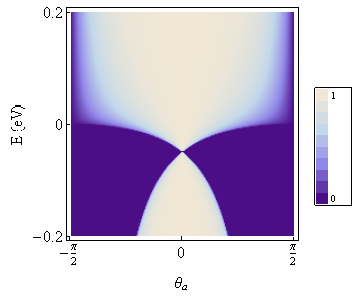
\includegraphics[scale=0.5]{images/step-1}}
				\caption{$V_{a}=0.05$ eV, $V_{b}=-0.05$ eV}
			\end{subfigure}
			\hspace{0.5cm}
			\begin{subfigure}[h]{0.5\textwidth}
				\centerline{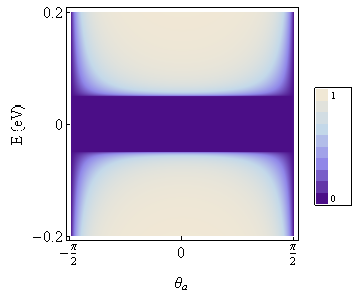
\includegraphics[scale=0.5]{images/step-2}}
				\caption{$m_{a}=0.05$ eV and $m_{b}=0$ eV}
			\end{subfigure}
			\caption{Density plots for the transmission probability against energy and incident angle for a graphene step from Equation (\ref{stept}).}
			\label{step-1}
		\end{figure}
		\begin{figure}[h]
			\begin{subfigure}[h]{0.5\textwidth}
				\centerline{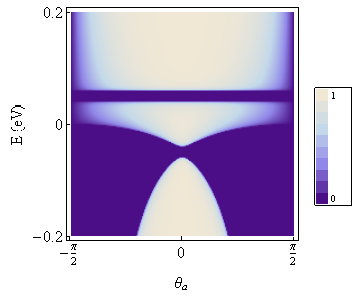
\includegraphics[scale=0.5]{images/step-3}}
				\caption{$V_{a}=0.05$ eV, $V_{b}=-0.05$ eV, $m_{a,b}=0.01$ eV}
			\end{subfigure}
			\hspace{0.5cm}
			\begin{subfigure}[h]{0.5\textwidth}
				\centerline{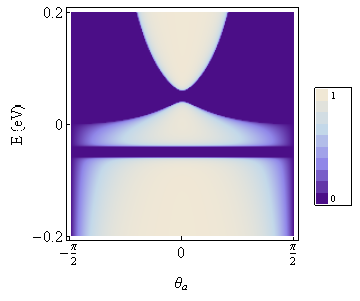
\includegraphics[scale=0.5]{images/step-4}}
				\caption{$V_{a}=-0.05$ eV, $V_{b}=0.05$ eV, $m_{a,b}=0.01$ eV}
			\end{subfigure}
			\caption{Density plots for the transmission probability against energy and incident angle for massive graphene potential step from Equation (\ref{stept}). These plots show opposing properties when the potentials are flipped.}
			\label{step-3}
		\end{figure}
%%%%%
%%%%%
%%%%%
%%%%%
%%%%%
		\section{IV Characteristics at Finite Temperatures}
		\label{Potential Step - IV Characteristics at Finite Temperatures}
			The transmission properties in Section \ref{Potential Step - Transfer and Scattering Matrices} can then be used to find the current through a scattering device. Using the Landauer formalism in Section \ref{Introduction - Landauer Formalism in Graphene} the current dependence on voltage, step height, temperature and energy gap can be obtained numerically.
			
			In Figure \ref{step-ivg-500} and Figure \ref{step-ivg-m}, current is plotted against step height. The symmetrical potential step is strongly affected by the direction of the step. When $V_{a}$ is larger than $V_{b}$ the current is overall much higher. This difference is most noticeable when the magnitude of the step is about $0.1$ eV. As expected when the direction of the step, or the external voltage is reversed the current through the step is reversed.

			When an energy gap is included the maximum value of the current is reduced. If the energy gap is present in both regions, two regions of low current will occur either side of a peak created at $V_{g}=0$. As the energy gap increases in magnitude these regions of low current will produce zero current for certain step heights. If only one step region has an energy gap, a single area of low current will occur at the step height of that step region. These effects can be seen in Figure \ref{step-ivg-m}.
		\begin{figure}[h]
			 \begin{subfigure}[h]{0.3\textwidth}
				\centerline{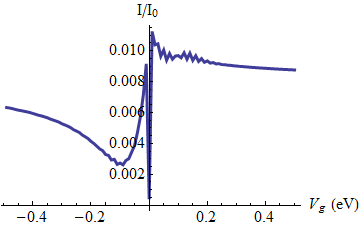
\includegraphics[scale=0.35]{images/step-vg-1}}
				\caption{$V_{sd}=0.1$ V, $V_{a}=V_{g}$ and $V_{b}=-V_{g}$.}
			\end{subfigure}
			\hspace{0.5cm}
			\begin{subfigure}[h]{0.3\textwidth}
				\centerline{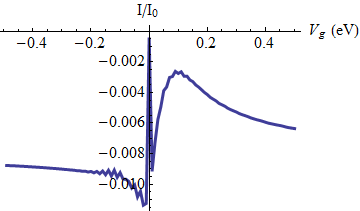
\includegraphics[scale=0.35]{images/step-vg-2}}
				\caption{$V_{sd}=-0.1$ V, $V_{a}=V_{g}$ and $V_{b}=-V_{g}$.}
			\end{subfigure}
			\hspace{0.5cm}
			\begin{subfigure}[h]{0.3\textwidth}
				\centerline{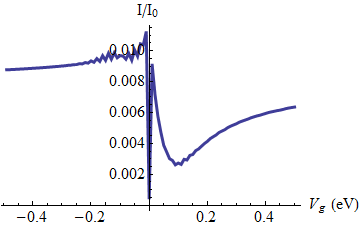
\includegraphics[scale=0.35]{images/step-vg-3}}
				\caption{$V_{sd}=0.1$ V, $V_{a}=-V_{g}$ and $V_{b}=V_{g}$.}
			\end{subfigure}
			\caption{Current against step height for symmetrical graphene potential steps from Equation (\ref{introduction-i-graphene}) with the transmission probability from Equation (\ref{stept}). For all plots $t=298$ K.}
			\label{step-ivg-500}
		\end{figure}
		\begin{figure}[h]
			 \begin{subfigure}[h]{0.3\textwidth}
				\centerline{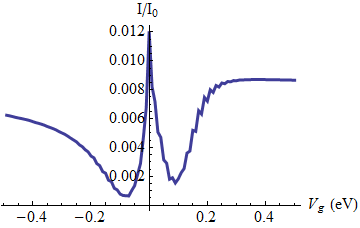
\includegraphics[scale=0.35]{images/step-vgm-1}}
				\caption{ $m_{a,b}=0.05$ eV.}
			\end{subfigure}
			\hspace{0.5cm}
			\begin{subfigure}[h]{0.3\textwidth}
				\centerline{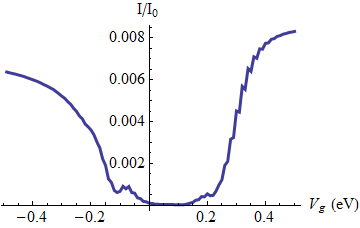
\includegraphics[scale=0.35]{images/step-vgm-2}}
				\caption{$m_{a}=0.2$ eV and $m_{b}=0$ eV.}
			\end{subfigure}
			\hspace{0.5cm}
			\begin{subfigure}[h]{0.3\textwidth}
				\centerline{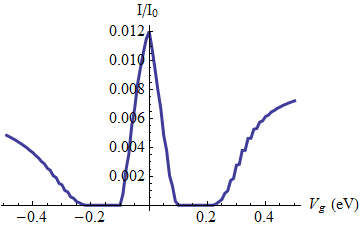
\includegraphics[scale=0.35]{images/step-vgm-3}}
				\caption{$m_{a,b}=0.2$ eV.}
			\end{subfigure}
			\caption{Current against step height for massive symmetrical graphene potential steps from Equation (\ref{introduction-i-graphene}) with the transmission probability from Equation (\ref{stept}). For all plots $V_{a}=V_{g}$, $V_{b}=-V_{g}$, $V_{sd}=0.1$ V and $t=298$ K.}
			\label{step-ivg-m}
		\end{figure}

			For a step with a fixed height the voltage across the device can be varied. Figure \ref{step-iv} shows current against source-drain voltage for a variety of graphene steps. The current through a symmetrical potential step appears to have a bias towards the positive voltages when $V_{a}>V_{b}$. This property is reversed if the step heights are reversed therefore a p-n diode is bias in the positive direction, where an n-p diode is bias in the negative direction. When an energy gap is included as in Figure \ref{step-iv} (c), the region of zero (or very low) current is expanded. Similar results were shown using the WKB method for graphene p-n junctions in \cite{b48}, relating the low current region to the voltage bias in Zener diodes and experimentaly in \cite{b57} for p-i-n diodes. 
		\begin{figure}[h]
			 \begin{subfigure}[h]{0.3\textwidth}
				\centerline{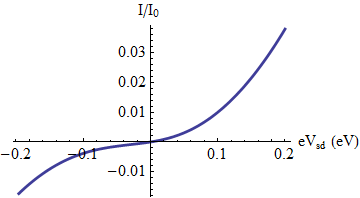
\includegraphics[scale=0.35]{images/step-v-1}}
				\caption{$V_{a}=0.05$ eV and $V_{b}=-0.05$ eV.}
			\end{subfigure}
			\hspace{0.5cm}
			\begin{subfigure}[h]{0.3\textwidth}
				\centerline{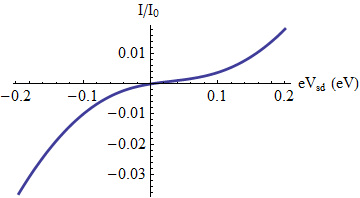
\includegraphics[scale=0.35]{images/step-v-2}}
				\caption{$V_{a}=-0.05$ eV and $V_{b}=0.05$ eV.}
			\end{subfigure}
			\hspace{0.5cm}
			\begin{subfigure}[h]{0.3\textwidth}
				\centerline{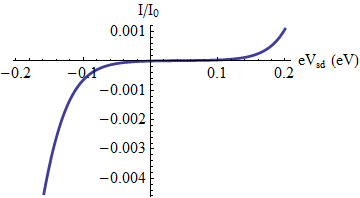
\includegraphics[scale=0.35]{images/step-v-3}}
				\caption{$V_{a}=0.05$ eV, $V_{b}=-0.05$ eV and $m_{a}=0.2$ eV.}
			\end{subfigure}
			\caption{Current against source-drain voltage for graphene potential steps from Equation (\ref{introduction-i-graphene}) with the transmission probability from Equation (\ref{stept}). For all plots $t=298$ K.}
			\label{step-iv}
		\end{figure}

			The temperature dependence on current for graphene steps is then shown in Figure \ref{step-it}. The direction of the step again contributes largely to the current at low temperatures. The current is over double when $V_{a}>V_{b}$, however, the current through the step appears to become fairly linear at higher temperatures, reducing the effect voltage and step direction has on the current. The addition of an energy gap lowers the overall current, this effect is most obvious at low temperatures. A large energy gap can reduce the current to essentially zero at lower temperatures until the linear nature of the temperature dependence re-emerges at high temperatures.
		\begin{figure}[h]
			 \begin{subfigure}[h]{0.3\textwidth}
				\centerline{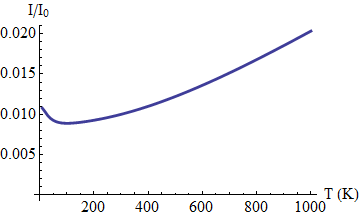
\includegraphics[scale=0.35]{images/step-t-1}}
				\caption{$V_{a}=0.05$ eV and $V_{b}=-0.05$ eV.}
			\end{subfigure}
			\hspace{0.5cm}
			\begin{subfigure}[h]{0.3\textwidth}
				\centerline{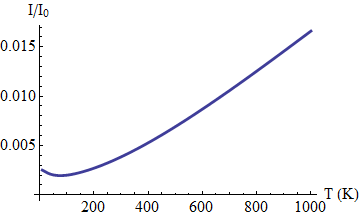
\includegraphics[scale=0.35]{images/step-t-3}}
				\caption{$V_{a}=-0.05$ eV and $V_{b}=0.05$ eV.}
			\end{subfigure}
			\hspace{0.5cm}
			\begin{subfigure}[h]{0.3\textwidth}
				\centerline{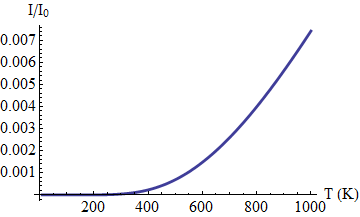
\includegraphics[scale=0.35]{images/step-t-2}}
				\caption{$V_{a}=0.05$ eV, $V_{b}=-0.05$ eV and $m_{a}=0.2$ eV.}
			\end{subfigure}
			\caption{Current against temperature for graphene potential steps from Equation (\ref{introduction-i-graphene}) with the transmission probability from Equation (\ref{stept}). For all plots $V_{sd}=0.1$ V.}
			\label{step-it}
		\end{figure}
%%%%%
%%%%%
%%%%%
%%%%%
%%%%%
		\section{Conductance}
		\label{Potential Step - Conductance}
			Following on from the current, the conductance of a sample can also be obtained. The non-infinite, zero temperature conductance formula was discussed in Section \ref{Introduction - Landauer Formalism in Graphene}. The numerical plots for zero temperature conductance with small source-drain voltages is shown in Figure \ref{step-g} for various graphene steps.
				
			At energies outside of the step the conductance follows a very linear dependence on energy. This is caused by the inclusion of the $|E_{f}|$ term from the graphene density of states. Inside the step the conductance increases away from zero and lowest step height. When the Fermi energy is equal to zero or the lowest step height the conductance reduces to zero. The conductance is also reduced to zero if an energy gap is included; the region of zero conductance is equivalent to the magnitude of the energy gap.
		\begin{figure}[h]
			 \begin{subfigure}[h]{0.3\textwidth}
				\centerline{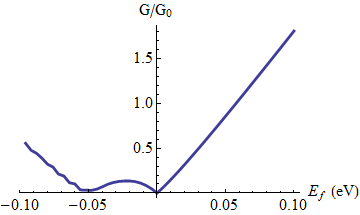
\includegraphics[scale=0.35]{images/step-g-1}}
				\caption{$V_{a}=0.05$ eV and $V_{b}=-0.05$ eV.}
			\end{subfigure}
			\hspace{0.5cm}
			\begin{subfigure}[h]{0.3\textwidth}
				\centerline{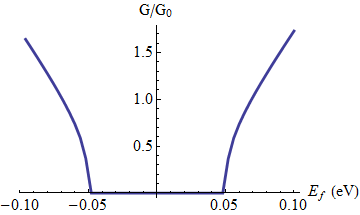
\includegraphics[scale=0.35]{images/step-g-2}}
				\caption{$m_{a}=0.05$ eV and $m_{b}=0$ eV.}
			\end{subfigure}
			\hspace{0.5cm}
			\begin{subfigure}[h]{0.3\textwidth}
				\centerline{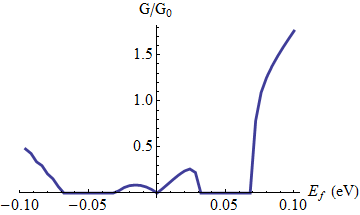
\includegraphics[scale=0.35]{images/step-g-3}}
				\caption{$V_{a}=0.05$ eV, $V_{b}=-0.05$ eV and $m_{a,b}=0.2$ eV.}
			\end{subfigure}
			\caption{The zero temperature conductance with small source-drain voltages has been plotted against Fermi energy for various graphene steps. The conductance is taken from Equation (\ref{introduction-g-zero}) with the step transmission probability from Equation (\ref{stept}).} 
			\label{step-g}
		\end{figure}
%\end{document}
	%\documentclass[12pt,a4paper]{report}
%\usepackage[utf8]{inputenc}
%\usepackage{amsmath}
%\usepackage{amsfonts}
%\usepackage{amssymb}
%\usepackage[margin=2.5cm]{geometry}
%\usepackage{graphicx}
%\usepackage{caption}
%\usepackage{subcaption}
%\usepackage[nottoc,numbib]{tocbibind}
%\linespread{1.3}
%\begin{document}
\chapter{Rectangular Barrier}
\label{Rectangular Barrier}
	In this section the transport properties for massive Dirac fermions through a potential barrier will be examined. This problem was originally studied with respect to potential barriers \cite{b12}, but has been expanded to include magnetic field \cite{b14} and energy gaps \cite{b4,b13,b15,b16,b17}. The massive rectangular potential barrier can be split into seven transmission regions shown in Figure \ref{rectangular-barrier-regions-flat} (a) and three different wave-function regions shown in Figure \ref{rectangular-barrier-regions-flat} (b). The first region of transport in Figure \ref{rectangular-barrier-regions-flat} (a) is below the Fermi level therefore only hole transport exists; transmission, reflection, resonances and Klein tunnelling can occur here. In region 2 $\hbar v_{f}k_{y}$ is larger than energy $E$, this is a region of hole transport shifted by the potential into a non-valid energy region allowing bound states to occur within the barrier but decay outside. Region 3 shows electron-hole transport within the potential barrier, pure oscillatory solutions provide similar properties to region 1. Region 4 is a region of no propagation that has been shifted by the potential. Energy is no longer less than $\hbar v_{f}k_{y}$, however, it maintains the properties of a region of no propagation. This region is responsible for the drop in transmission probability at $E\approx V$. Region 5 is above the barrier, pure electron transport again shows similar properties to region 1. In region 6 energy is less than $\hbar v_{f}k_{y}$, therefore no propagation can occur here. For massive quasiparticles the 7th region must be included, here the energy gap introduces extra regions of no propagation caused by the gap in the energy spectrum before and inside the barrier. These seven regions can then be applied to Figure \ref{rectangular-barrier-regions-flat} (b); region 1 occurs at energies below zero energy, regions 2, 3 occurs within the barrier, region 4 is  located where energy is close to barrier height, region 5 occurs above the barrier and region 7 is between the gaps in the energy spectrum. As the energy $E$ cannot be lower than $\hbar v_{f}k_{y}$ region 6 cannot be shown on Figure \ref{rectangular-barrier-regions-flat} (b).
\begin{figure}
	\begin{subfigure}{0.45\textwidth}
		\centerline{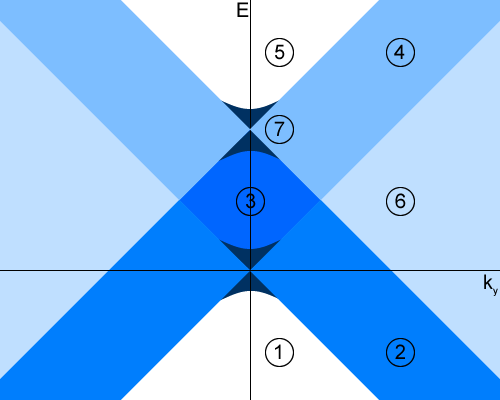
\includegraphics[scale=0.4]{images/rectangular-barrier-regions-flat}}
		\caption{}
	\end{subfigure}
	\hspace{1.2cm}
	\begin{subfigure}{0.45\textwidth}
		\centerline{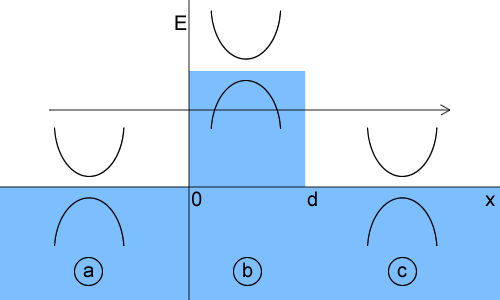
\includegraphics[scale=0.45]{images/potential-constant-mass-barrier-flat}}
		\caption{}
	\end{subfigure}
	\caption{(a) The seven independent regions of transmission for massive quasiparticles in a potential barrier. Six regions exist for a massless graphene potential barrier. The seventh region is caused by the introduction of an energy gap into the graphene spectrum. (b) The three wave-function regions a, b and c for massive quasiparticles in a potential barrier. Also shown is the parabolic dispersion relation and band gap caused by an energy gap in the graphene Hamiltonian.}
	\label{rectangular-barrier-regions-flat}
\end{figure}
%%%%%
%%%%%
%%%%%
	\section{Transfer Matrix}
	\label{Rectangular Barrier - Transfer Matrix}
		This section shows the transfer matrix method for solving the massive rectangular potential barrier. Oscillatory wave-functions with mass and potential will be used in all three regions. The subscript lettering for $q, \theta, V, m$ and $\alpha$ has been introduced to seperate constants in the corresponding barrier regions in Figure \ref{rectangular-barrier-regions-flat} (b). The normalised wave-functions in regions $a,b$ and $c$ can be taken from Section \ref{Wave-functions - Oscillitary}:
			\begin{align}
				\psi\left(x,y\right)_{a,b,c}=
				c_{a,b,a}e^{ik_{y}y}
				\left[\begin{array}{ccc}
					e^{iq_{a,b,a}x}&e^{-iq_{a,b,a}x}\\
					\alpha_{a,b,a}e^{iq_{\left(a,b,a\right)}x+i\theta_{a,b,a}}&-\alpha_{a,b,a}e^{-iq_{a,b,a}x-i\theta_{a,b,a}}
				\end{array}\right]
				\left[\begin{array}{ccc}
					a_{1,3,5}\\
					a_{2,4,6}
				\end{array}\right]
			\end{align}
			The continuity of wave-functions requires that at the first barrier interface $x=d_{1}$, the wave-function $\psi_{a}$ must be equal to $\psi_{b}$. In matrix form this can be written as:
			\begin{align}
				c_{a}
				\left[\begin{array}{ccc}
					e^{iq_{a}d_{1}}&e^{-iq_{a}d_{1}}\\
					\alpha_{a}e^{iq_{a}d_{1}+i\theta_{a}}&-\alpha_{a}e^{-iq_{a}d_{1}-i\theta_{a}}
				\end{array}\right]
				\left[\begin{array}{ccc}
					a_{1}\\
					a_{2}
				\end{array}\right]
				&=
				c_{b}
				\left[\begin{array}{ccc}
					e^{iq_{b}d_{1}}&e^{-iq_{b}d_{1}}\\
					\alpha_{b}e^{iq_{b}d_{1}+i\theta_{b}}&-\alpha_{b}e^{-iq_{b}d_{1}-i\theta_{b}}
				\end{array}\right]
				\left[\begin{array}{ccc}
					a_{3}\\
					a_{4}
				\end{array}\right]
			\end{align}
			For simplicity the matrices $m_{1}$ and $m_{2}$ have been introduced to represent the wave-functions on either side of the interface so that:
			\begin{align}
				m_{1}\left[\begin{array}{ccc}
					a_{1}\\
					a_{2}
				\end{array}\right]
				&=
				m_{2}\left[\begin{array}{ccc}
					a_{3}\\
					a_{4}
				\end{array}\right]
			\end{align}
			At the second barrier interface $x=d_{2}$, continuity requires that $\psi_{b}$ must be equal to $\psi_{c}$:
			\begin{align}
				c_{b}
				\left[\begin{array}{ccc}
					e^{iq_{b}d_{2}}&e^{-iq_{b}d_{2}}\\
					\alpha_{b}e^{iq_{b}d_{2}+i\theta_{b}}&-\alpha_{b}e^{-iq_{b}d_{2}-i\theta_{b}}
				\end{array}\right]
				\left[\begin{array}{ccc}
					a_{3}\\
					a_{4}
				\end{array}\right]
				&=
				c_{a}
				\left[\begin{array}{ccc}
					e^{iq_{a}d_{2}}&e^{-iq_{a}d_{2}}\\
					\alpha_{a}e^{iq_{a}d_{2}+i\theta_{a}}&-\alpha_{a}e^{-iq_{a}d_{2}-i\theta_{a}}
				\end{array}\right]
				\left[\begin{array}{ccc}
					a_{5}\\
					a_{6}
				\end{array}\right]
			\end{align}
			Here $m_{3}$ and $m_{4}$ will be introduced to represent the wave-functions on either side of the barrier interface so that:
			\begin{align}
				m_{3}\left[\begin{array}{ccc}
					a_{3}\\
					a_{4}
				\end{array}\right]
				&=
				m_{4}\left[\begin{array}{ccc}
					a_{5}\\
					a_{6}
				\end{array}\right]
			\end{align}
			With these matrices the constants $a_{3}$ and $a_{4}$ can be removed and the transfer matrix $M$ becomes:
			\begin{align}
				\left[\begin{array}{ccc}
					a_{5}\\
					a_{6}
				\end{array}\right]=M
				\left[\begin{array}{ccc}
					a_{1}\\
					a_{2}
				\end{array}\right]\hspace{1cm}
				M=m_{4}^{-1}m_{3}m_{2}^{-1}m_{1}
			\end{align}
			The barrier interfaces can be set to $d_{1}=0$ and $d_{2}=d$ to produce the matrix elements:
				\begin{align}
					M_{1,1}&=\frac{e^{-iq_{a}d}\left(2\alpha_{a}\alpha_{b}\cos(\theta_{a})\cos(\theta_{b})\cos(q_{b}d)-i\sin(q_{b}d)\left(2\alpha_{a}\alpha_{b}\sin(\theta_{a})\sin(\theta_{b})-\alpha_{a}^{2}-\alpha_{b}^{2}\right)\right)}{2\alpha_{a}\alpha_{b}\cos(\theta_{a})\cos(\theta_{b})}\\
					M_{1,2}&=\frac{e^{-iq_{a}d}2i\sin(q_{b}d)\left(\alpha_{b}^{2}-\alpha_{a}\alpha_{b}e^{-i\theta_{a}}2i\sin(\theta_{b})-\alpha_{a}^{2}e^{-2i\theta_{a}}\right)}{2\alpha_{a}\alpha_{b}\cos(\theta_{a})\cos(\theta_{b})}\\
					M_{2,1}&=-\frac{e^{iq_{a}d}2i\sin(q_{b}d)\left(\alpha_{b}^{2}+\alpha_{a}\alpha_{b}e^{-i\theta_{a}}2i\sin(\theta_{b})-\alpha_{a}^{2}e^{-2i\theta_{a}}\right)}{2\alpha_{a}\alpha_{b}\cos(\theta_{a})\cos(\theta_{b})}\\
M_{2,2}&=\frac{e^{iq_{a}d}\left(2\alpha_{a}\alpha_{b}\cos(\theta_{a})\cos(\theta_{b})\cos(q_{b}d)+i\sin(q_{b}d)\left(2\alpha_{a}\alpha_{b}\sin(\theta_{a})\sin(\theta_{b})-\alpha_{a}^{2}-\alpha_{b}^{2}\right)\right)}{2\alpha_{a}\alpha_{b}\cos(\theta_{a})\cos(\theta_{b})}
				\end{align}
				This transfer matrix satisfies all of the following properties \cite{b18}, which shows that the transfer matrix is valid.
				\begin{align}
					\det(M)=1\hspace{1cm}M_{1,1}=M_{2,2}^{*}\hspace{1cm}M_{1,2}=M_{2,1}^{*}
				\end{align}
				Using this matrix the transmission coefficient can easily be found as it is known that the constants have the following values: $a_{1}=1, a_{2}=r, a_{3}=t$ and $a_{4}=0$
				\begin{align}
					\left[\begin{array}{ccc}
						t\\
						0
					\end{array}\right]=
					\left[\begin{array}{ccc}
						M_{11}&M_{12}\\
						M_{21}&M_{22}
					\end{array}\right]
					\left[\begin{array}{ccc}
						1\\
						r
					\end{array}\right]\hspace{1cm}
					t=\frac{1}{M_{22}}\hspace{1cm}T=|t|^{2}
				\end{align}
				Then the transmission probability $T$ can be calculated as:
				\begin{equation}
					T=\frac{4\alpha_{a}^{2}\alpha_{b}^{2}\cos^{2}(\theta_{a})\cos^{2}(\theta_{b})}{4\alpha_{a}^{2}\alpha_{b}^{2}\cos^{2}(q_{b}d)\cos^{2}(\theta_{a})\cos^{2}(\theta_{b})+\sin^{2}(q_{b}d)\left(2\alpha_{a}\alpha_{b}\sin(\theta_{a})\sin(\theta_{b})-\alpha_{a}^{2}-\alpha_{b}^{2}\right)^{2}}
					\label{eq:transmission}
				\end{equation}
				This result includes an energy gap and potential term. If the respective energy gap, or potential term is set to zero the results in \cite{b1} can be obtained. When potentials approach the electron mass $V \approx m_{e}c^{2}$ \cite{b49}, $\theta_{b}\rightarrow 0$ and the transmission probability reduces to the result for Klein tunnelling shown in \cite{b12}:
				\begin{equation}
					T=\frac{\cos^{2}(\theta_{a})}{1-\cos^{2}(q_{b}d)\sin^{2}(\theta_{a})}
					\label{t2}
				\end{equation}
				The result in Equation (\ref{eq:transmission}) is then plotted in Figure \ref{transmissionplot}. This result can be reduced to the graphene potential barrier in Figure \ref{transmissionplot} (a), a region of finite mass in Figure \ref{transmissionplot} (b) or the massive potential barrier shown in Figure \ref{transmissionplot} (c). The potential barrier features $T=1$ when $\theta_{a}=0$ for all energies with exception of $E=V_{a,b}$ and shows clear resonances. The introduction of a region of finite mass creates a region of no propagation centered at $E=0$, with symmetrical transmission probability outside of this gap. The massive potential barrier shows properties of both of these cases, the asymetrical transmission probability on the energy axis from the potential barrier and the regions of no propagation from the region of finite mass. Under the condition of Klein tunnelling ($V\approx m_{e}c^{2}$) all of these barriers experience perfect transmission with the exception of inside the gap regions. Inside the gap regions the transmission probability approaches zero but sharply increases to one outside.
\begin{figure}
	\begin{subfigure}{0.3\textwidth}
		\centerline{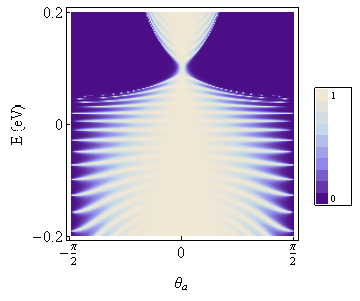
\includegraphics[scale=0.43]{images/potential}}
		\caption{$m_{a,b}=0$ eV and $V_{b}=0.1$ eV.}
	\end{subfigure}
	\hspace{0.5cm}
	\begin{subfigure}{0.3\textwidth}
		\centerline{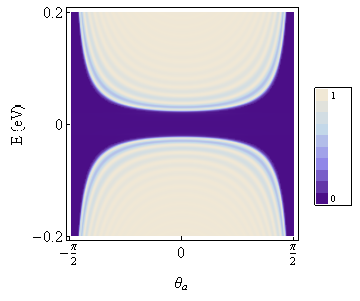
\includegraphics[scale=0.43]{images/mass}}
		\caption{$m_{a}=0$ eV, $m_{b}=0.02$ eV and $V_{b}=0$ eV.}
	\end{subfigure}
	\hspace{0.5cm}
	\begin{subfigure}{0.3\textwidth}
		\centerline{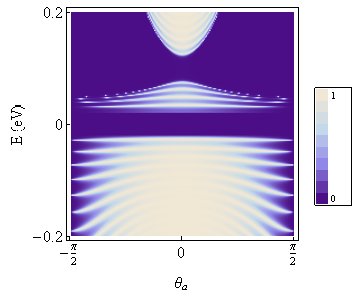
\includegraphics[scale=0.43]{images/transmission}}
		\caption{$m_{a,b}=0.02$ eV and $V_{b}=0.1$ eV.}
	\end{subfigure}
	\caption{Density plots of transmission probability $T$ against energy $E$ and incident angle $\theta_{a}$ from Equation (\ref{eq:transmission}). In all plots the width $d=200$ nm and $V_{a}=0$ eV. (a) Shows results for the potential barrier with gapless Dirac spectrum. (b) Massless Dirac fermions entering a region of finite mass. (c) Massive quasiparticles transmit through a potential barrier.}
	\label{transmissionplot}
\end{figure}

				In Figure \ref{thinbarrier} (a) the transmission probability is plotted with the depenence on energy gap. At larger values of energy gap it can be seen that the gap region increases fairly linearly, however at small energy gaps there is a non-negligible transmission probability. Similarly in Figure \ref{thinbarrier} (b) the dependence of barrier width on transmission probability is shown. Here as width increases the number of resonances increases. For thin barriers a finite transmission probability occurs at all energies, again removing the effect of the energy gap.
\begin{figure}
	\begin{subfigure}{0.45\textwidth}
		\centerline{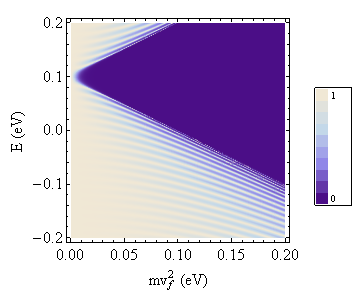
\includegraphics[scale=0.5]{images/contour-t-m}}
		\caption{$m_{a}=0$ eV, $V_{a}=0$ eV, $V_{b}=0.1$ eV and $d=200$ nm.}
	\end{subfigure}
	\hspace{1.2cm}
	\begin{subfigure}{0.45\textwidth}
		\centerline{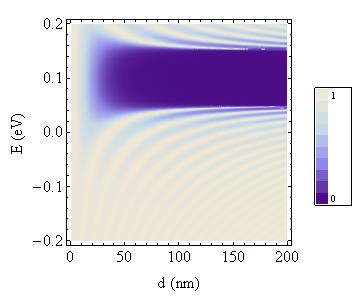
\includegraphics[scale=0.5]{images/mass-potential-e-d}}
		\caption{$m_{b}=0.05$ eV, $m_{a}=0$ eV, $V_{a}=0$ eV and $V_{b}=0.1$ eV.}
	\end{subfigure}
	\caption{Density plots of transmission probability against energy gap and barrier width. In (a) The transmission properties with a varying energy gap. (b) The dependence of barrier width $d$ on the transmission probability.}
	\label{thinbarrier}
\end{figure}
%%%%%
%%%%%
%%%%%
			\section{Fabry-P\'{e}rot Resonances}
			\label{Rectangular Barrier - Fabry-Perot Resonances}
				A single graphene barrier can act as a Fabry-P\'{e}rot resonator \cite{b38}. At resonance the transmission probability $T$ will be equal to one. It is clear from Equation (\ref{eq:transmission}) that this requirement is met when $q_{b}d=n\pi$. Evaluating this relation provides the energies where the Fabry-P\'{e}rot resonances can be found.
				\begin{equation}
					E=V_{b}\pm\sqrt{\hbar^{2}v_{f}^{2}\left(\frac{n^{2}\pi^{2}}{d^{2}}+k_{y}^{2}\right)+m_{b}^{2}}
					\label{resonances-barrier}
				\end{equation}
				The condition of $E=\hbar v_{f}k_{y}$ is the limit of where real solutions exist. This condition can be applied to Equation (\ref{resonances-barrier}), which then becomes:
				\begin{equation}
					E=\frac{V_{b}}{2}-\frac{v_{f}^{2}\hbar^{2}n^{2}\pi^{2}+d^{2}m_{b}^{2}}{2V_{b}d^{2}}
				\end{equation}
	Showing the energies at which real and imaginary solutions coincide. When an energy gap is introduced the gap centered around $V_{b}$ increases by $2m$. This increased gap reduces the energy region resonances can exist, resulting in a higher density of resonances. If the energy gap $m_{b}=0$ this result can be reduced to the gapless case in \cite{b14}. These resonances are not restricted to potential barriers; for the case of $V_{a,b}=0$, $m_{a}=0$ and $m_{b} \neq 0$ resonances can still be obtained.
\begin{figure}
	\centerline{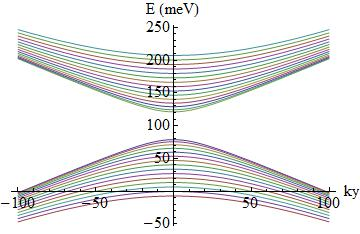
\includegraphics[scale=0.5]{images/mass-potential-energy-levels}}
	\label{}
	\caption{The dependence of energy $E$ and $k_{y}$ on Fabry-P\'{e}rot resonances as described by Equation (\ref{resonances-barrier}) with $\hbar v_{f}=1$. Here the barrier has the properties $m_{a,b}=0.02$ eV, $V_{b}=0.1$ eV, $V_{a}=0$ eV and width $d=200$ nm.}
\end{figure}
%%%%%
%%%%%
%%%%%
			\section{Bound States}
			\label{Rectangular Barrier - Bound States}
				A bound state will only be found within a barrier, therefore the wave-functions must decay outside of the barrier. To find the bound states within a potential barrier the wave-function system of growth-oscillatory-decay shown in Figure \ref{bound-states} is needed. Using the wave-functions derived in Section \ref{Wave-functions - Growth and Decay} and Section \ref{Wave-functions - Oscillitary} this system can be constructed. The wave-functions in each region take the form:
				\begin{align}
					\psi_{a}=a_{1}
					\left[\begin{array}{ccc}
						e^{q_{d}x}\\
						i\alpha_{-}e^{q_{d}x}
					\end{array}\right]e^{ik_{y}y}
				\end{align}
				\begin{align}
					\psi_{b}=
					\left[\begin{array}{ccc}
						e^{iqx}&e^{-iqx}\\
						\alpha e^{iqx+i\theta}&-\alpha e^{-iqx-i\theta}
					\end{array}\right]
					\left[\begin{array}{ccc}
						a_{2}\\
						a_{3}
					\end{array}\right]e^{ik_{y}y}
				\end{align}
				\begin{align}
					\psi_{c}=a_{4}
					\left[\begin{array}{ccc}
						e^{-q_{d}x}\\
						-i\alpha_{+}e^{-q_{d}x}
					\end{array}\right]e^{ik_{y}y}
				\end{align}
				At the boundaries $d_{1}$ and $d_{2}$ the continuity of wave-functions requires that $\psi_{a}=\psi_{b}$ and $\psi_{b}=\psi_{c}$. From this condition the set of simultaneous equations can be made:
				\begin{align}
					a_{1}e^{q_{d}d_{1}}&=a_{2}e^{iqd_{1}}+a_{3}e^{-iqd_{1}}\\
					-ia_{1}\alpha_{-}e^{q_{d}d_{1}}&=\alpha\left(a_{2}e^{iqd_{1}+i\theta}-a_{3}e^{-iqd_{1}-i\theta}\right)\\
					a_{2}e^{iqd_{2}}+a_{3}e^{-iqd_{2}}&=a_{4}e^{-q_{d}d_{2}}\\
					\alpha\left(a_{2}e^{iqd_{2}+i\theta}-a_{3}e^{-iqd_{2}-i\theta}\right)&=ia_{4}\alpha_{+}e^{-q_{d}d_{2}}
				\end{align}
				Re-arranging these to be equal to zero the matrix $m$ can be made:
				\begin{align}
					\left[\begin{array}{cccc}
						e^{q_{d}d_{1}}&-e^{iqd_{1}}&-e^{-iqd_{1}}&0\\
						-i\alpha_{-}e^{q_{d}d_{1}}&-\alpha e^{iqd_{1}+i\theta}&\alpha e^{-iqd_{1}-i\theta}&0\\
						0&e^{iqd_{2}}&e^{-iqd_{2}}&-e^{-q_{d}d_{2}}\\
						0&\alpha e^{iqd_{2}+i\theta}&-\alpha e^{-iqd_{2}-i\theta}&-i\alpha_{+}e^{-q_{d}d_{2}}\\
					\end{array}\right]
					\left[\begin{array}{cccc}
						a_{1}\\
						a_{2}\\
						a_{3}\\
						a_{4}\\
					\end{array}\right]=
					\left[\begin{array}{cccc}
						0\\
						0\\
						0\\
						0\\
					\end{array}\right]
				\end{align}
				To find non-trivial solutions set $\det(m)=0$, $d_{1}=0$ and $d_{2}=d$. From this the dispersion relation can be found:
				\begin{equation}
					\tan(qd)=-\frac{q_{d}q}{\frac{E^{2}-m_{a}m_{b}+V_{a}V_{b}-E\left(V_{a}+V_{b}\right)}{\hbar^{2}v_{f}^{2}}-k_{y}^{2}}
					\label{boundstates}
				\end{equation}
				When the energy gap is removed this result can be reduced to the results for the potential barrier with a Dirac spectrum shown in \cite{b3}. The effect of the energy gap on the bound states is similar that of the Fabry-P\'{e}rot resonances; the energy gap reduces the valid region for bound states to exist, which causes the peaks of the states to occur at lower energies within the barrier. If the energy gap is significantly large, states at higher energies may be lost until the valid energy region approaches zero.
\begin{figure}
	\begin{subfigure}{0.45\textwidth}
		\centerline{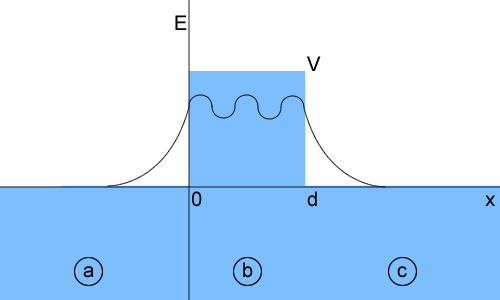
\includegraphics[scale=0.4]{images/bound-states}}
		\caption{}
		\label{}
	\end{subfigure}
	\hspace{1.2cm}
	\begin{subfigure}{0.45\textwidth}
		\centerline{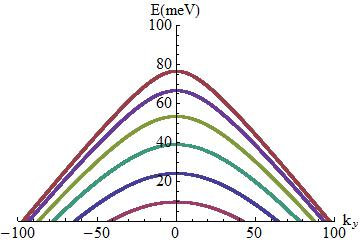
\includegraphics[scale=0.7]{images/bound-states-plot}}
		\caption{}
		\label{}
	\end{subfigure}
	\caption{(a) The required wave-function system to find bound states within a potential barrier. (b) The bound states found from Equation (\ref{boundstates}) within a potential barrier with massive quasiparticles where $\hbar v_{f}=1$, $m_{a,b}=0.02$ eV, $V_{b}=0.1$ eV, $V_{a}=0$ eV and the width $d=200$ nm.}
	\label{bound-states}
\end{figure}
%%%%%
%%%%%
%%%%%
		\section{Conductance}
		\label{Rectangular Barrier - Conductance}
	The conductance through a device can then be calculated via the Landauer formalism as described in Section \ref{Introduction - Landauer Formalism in Graphene}. In Figure \ref{pot-g-1} the conductance has been plotted against the Fermi level of the system. Experimentally this would be adjusted by applying a gate voltage to the substrate of the device \cite{b46}. In Figure \ref{pot-g-1} (a) and Figure \ref{pot-g-1} (b) the same barrier has been plotted at low temperature and at room temperature. It can be seen that the barrier creates minima at zero energy and at barrier height. Outside of the barrier region, the conductance becomes linear due to the graphene density of states. When the temperature is increased in Figure \ref{pot-g-1} (b) the barrier region smooths out reducing the effect of the potential. In Figure \ref{pot-g-1} (c) a small energy gap is included at zero and at barrier height, this creates regions of zero conductance centered at zero energy and at barrier height.
		\begin{figure}[h]
			 \begin{subfigure}[h]{0.3\textwidth}
				\centerline{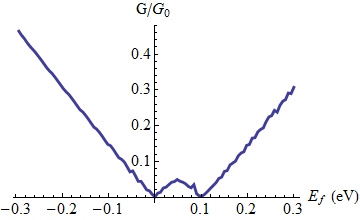
\includegraphics[scale=0.35]{images/pot-g-1}}
				\caption{$t=20$ K.}
			\end{subfigure}
			\hspace{0.5cm}
			\begin{subfigure}[h]{0.3\textwidth}
				\centerline{\includegraphics[scale=0.35]{images/pot-g-2}}
				\caption{$t=298$ K.}
			\end{subfigure}
			\hspace{0.5cm}
			\begin{subfigure}[h]{0.3\textwidth}
				\centerline{\includegraphics[scale=0.35]{images/pot-g-3}}
				\caption{$t=20$ K, $m_{a,b}=0.02$ eV.}
			\end{subfigure}
			\caption{Conductance against Fermi energy from Equation (\ref{introduction-g-t}) with the transmission probability in Equation (\ref{eq:transmission}). For all plots $V_{b}=0.1$ eV, $d=200$ nm and $eV_{sd}=0.01$ eV.}
			\label{pot-g-1}
		\end{figure}

	The height of the potential barrier is then adjusted in Figure \ref{pot-vg-1}, which would be caused by doping or interactions with a substrate. Figure \ref{pot-vg-1} (a) and Figure \ref{pot-vg-1} (b) show the dependence on barrier height at low temperatures. In Figure \ref{pot-vg-1} (a) the barrier height $V_{b}$ is adjusted, which shows oscillations caused by Fabry-P\'{e}rot resonances and an asymmetry between positive and negative gate voltages. In Figure \ref{pot-vg-1} (b) $V_{b}$ is kept constant at zero electron volts and the potential outside of region $b$ is adjusted to create a potential well or negative barrier. This shows very different results; the maximum conductance appears at zero gate voltage as with Figure \ref{pot-vg-1} (a), however, the conductance drops quickly as the sides of the well increase in height. Again there appears to be an asymmetry between the positive and negative gate voltages with negative voltages causing a sharp drop in conductance. In Figure \ref{pot-vg-1} (c) the conductance is then shown at room temperature ($298$ K). The overall conductance has increased, again with a maximum at zero gate voltage and an asymmetry between positive and negative gate voltages.
		\begin{figure}[h]
			 \begin{subfigure}[h]{0.3\textwidth}
				\centerline{\includegraphics[scale=0.35]{images/pot-vg-1}}
				\caption{$t=20$ K, $V_{b}=V_{g}$, $V_{a}=0$ eV.}
			\end{subfigure}
			\hspace{0.5cm}
			\begin{subfigure}[h]{0.3\textwidth}
				\centerline{\includegraphics[scale=0.35]{images/pot-vg-2}}
				\caption{$t=20$ K, $V_{a}=V_{g}$, $V_{b}=0$ eV.}
			\end{subfigure}
			\hspace{0.5cm}
			\begin{subfigure}[h]{0.3\textwidth}
				\centerline{\includegraphics[scale=0.35]{images/pot-vg-3}}
				\caption{$t=298$ K, $V_{b}=V_{g}$, $V_{a}=0$ eV.}
			\end{subfigure}
			\caption{Conductance against barrier height from Equation (\ref{introduction-g-t}) with the transmission probability in Equation (\ref{eq:transmission}). For all plots $d=200$ nm and $eV_{sd}=0.01$ eV.}
			\label{pot-vg-1}
		\end{figure}

	The conductance dependence on temperature is further examined in Figure \ref{pot-t-1}. At higher temperatures the dependence becomes linear, however at lower temperatures some differing properties can be observed. When $V_{b}$ is adjusted the conductance with respect to temperature increases faster then when $V_{a}$ is adjusted, corresponding to the higher conductances shown in Figure \ref{pot-vg-1} (a) and Figure \ref{pot-t-1} (b). When an energy gap is included in the spectrum the conductance is reduced significantly becoming close to zero. At higher temperatures the charge carriers have enough energy to escape the energy gap and the linear dependence is seen again.
		\begin{figure}[h]
			 \begin{subfigure}[h]{0.3\textwidth}
				\centerline{\includegraphics[scale=0.35]{images/pot-t-1}}
				\caption{$V_{b}=0.1$ eV, $V_{a}=0$ eV.}
			\end{subfigure}
			\hspace{0.5cm}
			\begin{subfigure}[h]{0.3\textwidth}
				\centerline{\includegraphics[scale=0.35]{images/pot-t-2}}
				\caption{$V_{b}=0.1$ eV, $V_{a}=0$ eV, $m_{a,b}=0.1$ eV.}
			\end{subfigure}
			\hspace{0.5cm}
			\begin{subfigure}[h]{0.3\textwidth}
				\centerline{\includegraphics[scale=0.35]{images/pot-t-3}}
				\caption{$V_{a}=0.1$ eV, $V_{b}=0$ eV.}
			\end{subfigure}
			\caption{Conductance against temperature from Equation (\ref{introduction-g-t}) with the transmission probability in Equation (\ref{eq:transmission}). For all plots $d=200$ nm and $eV_{sd}=0.01$ eV.}
			\label{pot-t-1}
		\end{figure}

	By adjusting the source-drain voltage through a potential barrier the conductance becomes similar to that of a semiconducting diode. Figure \ref{pot-vsd-1} shows the conductance dependence on source-drain voltage. By comparing the high and low temperature curves in Figure \ref{pot-vsd-1} (a) and Figure \ref{pot-vsd-1} (b) it can be seen that the current increases at lower voltages with increasing temperature. The effect of an energy gap is then shown in Figure \ref{pot-vsd-1} (c). Here a large energy gap causes the conductance to become near zero at low source-drain voltages. At higher voltages the conductance behaves similarly to the gapless case, although the gap region causes a much larger asymmetry between positive and negative voltages.
		\begin{figure}[h]
			 \begin{subfigure}[h]{0.3\textwidth}
				\centerline{\includegraphics[scale=0.35]{images/pot-vsd-1}}
				\caption{$T=20$ K.}
			\end{subfigure}
			\hspace{0.5cm}
			\begin{subfigure}[h]{0.3\textwidth}
				\centerline{\includegraphics[scale=0.35]{images/pot-vsd-2}}
				\caption{$T=298$ K.}
			\end{subfigure}
			\hspace{0.5cm}
			\begin{subfigure}[h]{0.3\textwidth}
				\centerline{\includegraphics[scale=0.35]{images/pot-vsd-3}}
				\caption{$T=298$ K and $m_{a,b}=0.1$ eV.}
			\end{subfigure}
			\caption{Conductance against source-drain voltage from Equation (\ref{introduction-g-t}) with the transmission probability in Equation (\ref{eq:transmission}). For all plots $d=200$ nm and $V_{b}=0.1$ eV.}
			\label{pot-vsd-1}
		\end{figure}
%%%%%
%%%%%
%%%%%
		\section{Conductance Without Graphene Density of States}
		\label{Rectangular Barrier - Conductance Withount Graphene Density of States}
			If the graphene density of states is not used in the derivation for conductance, a system where graphene is only used as a scattering device can be simulated. The result for the transmission probability from Equation (\ref{eq:transmission}) can then be used to calculate the conductance through a nano-device. In this way these results will be comparable to results obtained experimentally. The conductance at zero temperature without the graphene density of states is then \cite{b4, b13, b16}:
			\begin{equation}
				G=G_{0}\int^{\pi/2}_{-\pi/2}T\left(E_{f},\theta_{a}\right)\cos(\theta_{a})d\theta_{a}
				\label{g}
			\end{equation}
			where $G_{0}=2e^{2}/\hbar$ and $E_{f}$ is the Fermi energy. Figure \ref{rectangular-barrier-conductance-a} and Figure \ref{rectangular-barrier-conductance-c} then show the conductance for various barriers where energy gap and potential have been included within defined regions. From this, the effect of the energy gap is clearly shown as the conductance sharply decreases to zero within this region. When comparing the potential barriers it can also be seen that the overall conductance decreases and oscillations become more defined as the energy gap increases. In Figure \ref{rectangular-barrier-conductance-c} (b) a single conductance curve is examined. In this figure the energies at which the peaks of the bound states occur (from Equation (\ref{boundstates})) have been included as dashed lines. It can then be seen that the troughs in conductance approximately coincide with these energies. With this in mind the energies half way between the bound states were also included as solid lines. These solid lines then approximately show the energies at which the peaks in the conductance occur.
\begin{figure}
	\begin{subfigure}{0.45\textwidth}
		\centerline{\includegraphics[scale=0.6]{images/rectangular-barrier-conductance-a}}
		\caption{$V_{b}=0.1$ eV.}
	\end{subfigure}
	\hspace{1.2cm}
	\begin{subfigure}{0.45\textwidth}
		\centerline{\includegraphics[scale=0.6]{images/rectangular-barrier-conductance-b}}
		\caption{$V_{b}=0.1$ eV and $m_{a,b}=0.02$ eV.}
	\end{subfigure}
	\caption{The conductance from Equation (\ref{g}) for various barriers with width $d=200$ nm.}
	\label{rectangular-barrier-conductance-a}
\end{figure}
\begin{figure}
	\begin{subfigure}{0.45\textwidth}
		\centerline{\includegraphics[scale=0.6]{images/rectangular-barrier-conductance-c}}
		\caption{$m_{b}=0.02$ eV.}
	\end{subfigure}
	\hspace{1.2cm}
	\begin{subfigure}{0.45\textwidth}
		\centerline{\includegraphics[scale=0.6]{images/rectangular-barrier-conductance-max}}
		\caption{$m_{a}=0$ eV, $m_{b}=0.02$ eV, $V_{a}=0$ eV and $V_{b}=0.1$ eV.}
		\label{conductance-max}
	\end{subfigure}
	\caption{The conductance from Equation (\ref{g}) for a various barriers with width $d=200$ nm. In (b) the dashed lines show peaks of the bound states from Equation (\ref{boundstates}) and solid lines are located at energies mid way between bound states.}
	\label{rectangular-barrier-conductance-c}
\end{figure}
%%%%%
%%%%%
%%%%%
			\section{n-Barriers}
			\label{Rectangular Barrier - n-Barriers}
				To adjust the transfer matrix method for multiple barriers a phase shift must be introduced for when the electron is travelling between barriers \cite{b18}. For convenience each barrier will be on its own $x$ axis, so that the first barrier starts at $x_{1}=0$ and the second barrier starts at $x_{2}=0$. The distance between the two axes will be defined as $d_{1}+l$. A diagram of the two energy axes and distance $l$ is shown in Figure \ref{n-barriers-x}.
				\begin{figure}[h]
					\centerline{\includegraphics[scale=0.5]{images/multiple-potential-barrier-flat}}
					\caption{A double potential barrier with distance $l$ between barriers. The double barrier shown is constructed of two single potential barriers on independent axes $x_{1}$ and $x_{2}$. The two barriers can be joined by introducing a phase shift between the barriers.}
					\label{n-barriers-x}
				\end{figure}

				Continuity of the wave-functions require that the transmitted wave from the first barrier must be matched to the incident wave of the second barrier. For convenience, this will be done at the point $x_{1}=d_{1}+l/2$ and $x_{2}=-l/2$. Using the continuity of the wave-functions, which were derived in Section \ref{Wave-functions - Oscillitary}, at the points $x_{1}=d_{1}+l/2$ and $x_{2}=-l/2$ produces the relation:
				\begin{align}
					\left[\begin{array}{cc}
						e^{iq\left(d+\frac{l}{2}\right)}&e^{-iq\left(d+\frac{l}{2}\right)}\\
						\alpha_{1}e^{iq\left(d+\frac{l}{2}\right)+i\theta}&-\alpha_{1}e^{-iq\left(d+\frac{l}{2}\right)-i\theta}\\
					\end{array}\right]
					\left[\begin{array}{cc}
						a_{15}\\
						a_{16}\\
					\end{array}\right]
					&=
					\left[\begin{array}{cc}
						e^{-iq\frac{l}{2}}&e^{iq\frac{l}{2}}\\
						\alpha_{1}e^{-iq\frac{l}{2}+i\theta}&-\alpha_{1}e^{iq\frac{l}{2}-i\theta}\\
					\end{array}\right]
					\left[\begin{array}{cc}
						a_{21}\\
						a_{22}\\
					\end{array}\right]
				\end{align}
				The matrices $m_{1}$ and $m_{2}$ have been introduced to represent the wave-functions from each barrier so that:
				\begin{align}
					m_{1}
					\left[\begin{array}{cc}
						a_{15}\\
						a_{16}\\
					\end{array}\right]
					&=m_{2}
					\left[\begin{array}{cc}
						a_{21}\\
						a_{22}\\
					\end{array}\right]
				\end{align}
				Making $a_{21}$ and $a_{22}$ the subject produces the transfer matrix for the region between the two barriers:
				\begin{align}
					\left[\begin{array}{cc}
						a_{21}\\
						a_{22}\\
					\end{array}\right]
					=\Lambda
					\left[\begin{array}{cc}
						a_{15}\\
						a_{16}\\
					\end{array}\right]
					\hspace{1cm}	
					\Lambda=m_{2}^{-1}m_{1}=
					\left[\begin{array}{cc}
						e^{iq\left(d_{1}+\frac{l}{2}\right)}&0\\
						0&e^{-iq\left(d_{1}+\frac{l}{2}\right)}\\
					\end{array}\right]
				\end{align}
				Using the phase shift between the two barriers the transfer matrix for $n$ barriers can be calculated from:
				\begin{align}
					M_{n}=\Lambda^{-1}\left(\Lambda M\right)^{n}
					\label{mn}
				\end{align}

				where $M$ is the transfer matrix for a single potential barrier and $M_{n}$ is the transfer matrix for the whole barrier structure. By keeping the independent region notation from the single barrier any barrier combination can be created this way, providing there is a region between barriers. However, this can make the already complex result very unmanageable. For this reason it is convenient to use similar barriers. Some results from the evaluated transmission can be seen in Figure \ref{doubletransmissionplot}. These results show similar charateristics to the single barriers; the potential barrier shows $T=1$ when $\theta_{a}=0$ and the massive barrier contains a gap region centered at $E=0$ eV with symmetry on the energy axis. The most obvious exception is the double barrier systems show far more resonances due to the two extra wave-function regions added with the extra barrier.
\begin{figure}
	\begin{subfigure}{0.5\textwidth}
		\centerline{\includegraphics[scale=0.6]{images/double-potential}}
		\caption{The double potential barrier with $V_{b}=0.05$ eV.}
		\label{doubletransmissionplota}
	\end{subfigure}
	\hspace{0.6cm}
	\begin{subfigure}{0.5\textwidth}
		\centerline{\includegraphics[scale=0.6]{images/double-mass}}
		\caption{The double mass barrier with $m_{b}=0.05$ eV.}
		\label{doubletransmissionplotb}
	\end{subfigure}
	\caption{Transmission probability for double barrier systems from the transfer matrix in Equation (\ref{mn}). For simplicity similar barriers are used where $d_{1,2}=50$ nm, $l=50$ nm and $\theta_{a}=\pi/4$.}
	\label{doubletransmissionplot}
\end{figure}

				The effect of these resonances can clearly be seen when comparing the conductance for a double barrier in Figure \ref{doubletransmissionplotg} (b) with the conductance for a single barrier in Figure \ref{rectangular-barrier-conductance-a}.
\begin{figure}
	\begin{subfigure}{0.5\textwidth}
		\centerline{\includegraphics[scale=0.6]{images/double-potential-mass}}
		\caption{$\theta_{a}=\pi/4$.}
		\label{doubletransmissionplotga}
	\end{subfigure}
	\hspace{0.6cm}
	\begin{subfigure}{0.5\textwidth}
		\centerline{\includegraphics[scale=0.6]{images/double-potential-g}}
		\caption{}
		\label{doublegplot}
	\end{subfigure}
	\caption{(a) Transmission probability from the transfer matrix in Equation (\ref{mn}). (b) Conductance plot for symmetrical double massive potential barrier calculated from Equation (\ref{g}) with the transmission probability from the transfer matrix in Equation (\ref{mn}). For both plots the barriers have the characteristics $d_{1,2}=50$ nm, $l=50$ nm, $V_{b}=0.05$ eV and $m_{b}=0.05$ eV.}
	\label{doubletransmissionplotg}
\end{figure}
%%%%%
%%%%%
%%%%%
			\section{Graphene Superlattice}
			\label{Rectangular Barrier - Graphene Superlattice}
			The graphene superlattice consists of an infinite number of potential barriers with equal spacing. This problem can be compared to the electron in a periodic potential field \cite{b32} and is shown in Figure \ref{periodic}.
			\begin{figure}[h]
				\centerline{\includegraphics[scale=0.5]{images/periodic}}
				\caption{A periodic potential with distance $a$ between barriers and a barrier with $d$.}
				\label{periodic}
			\end{figure}

			The wave-functions in each region can be taken from Section \ref{Wave-functions - Oscillitary}. In region $a$ the normalised wave-functions have the form:
			\begin{align}
				\psi_{a}=
				c_{a}e^{ik_{y}y}
				\left[\begin{array}{ccc}
					e^{iq_{a}x}&e^{-iq_{a}x}\\
					\alpha_{a} e^{iq_{a}x+i\theta_{a}}&-\alpha_{a} e^{-iq_{a}x-i\theta_{a}}
				\end{array}\right]
				\left[\begin{array}{ccc}
					a_{1}\\
					a_{2}
				\end{array}\right]
			\end{align}
			In region $b$ there is no external potential and the normalised wave-functions are:
			\begin{align}
				\psi_{b}=
				c_{b}e^{ik_{y}y}
				\left[\begin{array}{ccc}
					e^{iq_{b}x}&e^{-iq_{b}x}\\
					\alpha_{b} e^{iq_{b}x+i\theta_{b}}&-\alpha_{b} e^{-iq_{b}x-i\theta_{b}}
				\end{array}\right]
				\left[\begin{array}{ccc}
					a_{3}\\
					a_{4}
				\end{array}\right]
			\end{align}
			Requiring that the potentials in regions $a$ and $c$ are the same, the wave-functions in regions $a$ and $c$ will be equivalent but with a spacial displacement and a potential phase shift of $e^{ik\left(a+d\right)}$, where $a+d$ is the period of the periodic potential. Here the constant $k=2\pi n/L$ where $L$ is the length of the entire structure and $n$ is an integer. Therefore the wave-functions can be written as:
			\begin{align}
				\psi_{c}=
				c_{a}e^{ik\left(a+d\right)}e^{ik_{y}y}
				\left[\begin{array}{ccc}
					e^{iq_{a}\left(x-a-d\right)}&e^{-iq_{a}\left(x-a-d\right)}\\
					\alpha_{a} e^{iq_{a}\left(x-a-d\right)+i\theta_{a}}&-\alpha_{a} e^{-iq_{a}\left(x-a-d\right)-i\theta_{a}}
				\end{array}\right]
				\left[\begin{array}{ccc}
					a_{1}\\
					a_{2}
				\end{array}\right]
			\end{align}
			Continuity of the wave-functions at the barrier interfaces located at $x=0$ and $x=a$ produces a set of four simultaneous equations. In matrix form these equations can be written as:
			\begin{align}
				\left[\begin{array}{cccc}
					c_{a}&c_{a}&-c_{b}&-c_{b}\\
					c_{a}\alpha_{a}e^{i\theta_{a}}&-c_{a}\alpha_{a}e^{-i\theta_{a}}&-c_{b}\alpha_{b}e^{i\theta_{b}}&c_{b}\alpha_{b}e^{-i\theta_{b}}\\
					-c_{a}e^{ik\left(a+d\right)}e^{-iq_{a}d}&-c_{a}e^{ik\left(a+d\right)}e^{iq_{a}d}&e^{iq_{b}a}&e^{-iq_{b}a}\\
					-c_{a}\alpha_{a}e^{ik\left(a+d\right)}e^{-iq_{a}d+i\theta_{a}}&c_{a}\alpha_{a}e^{ik\left(a+d\right)}e^{iq_{a}d-i\theta_{a}}&c_{b}\alpha_{b} e^{iq_{b}a+i\theta_{b}}&-c_{b}\alpha_{b} e^{-iq_{b}a-i\theta_{b}}
				\end{array}\right]
				\left[\begin{array}{cccc}
					a_{1}\\
					a_{2}\\
					a_{3}\\
					a_{4}
				\end{array}\right]
				=
				\left[\begin{array}{cccc}
					0\\
					0\\
					0\\
					0
				\end{array}\right]
			\end{align}
			These equations can be solved by requiring that the determinant of this matrix is equal to zero. Evaluating this results in the dispersion relation:
			\begin{align}
				-\sin(q_{a}d)&\sin(q_{b}d)\left[\frac{\alpha_{a}}{\alpha_{b}}+\frac{\alpha_{b}}{\alpha_{a}}\right]+\sin(q_{a}d)\sin(q_{b}d)\sin(\theta_{a})\sin(\theta_{b})\\
				&+\cos(q_{a}d)\cos(q_{b}d)\cos(\theta_{a})\cos(\theta_{b})-\cos(2kd)\cos(\theta_{a})\cos(\theta_{b})=0
				\label{Rectangular Barrier band eq}
			\end{align}
			For simplicity the widths of the periodic potential barriers and wells have been made equivalent so that $a=d$. The roots of this equation produce the energy bands of a graphene superlattice shown in Figure \ref{superlattice-bands}.
			\begin{figure}
				\begin{subfigure}{0.5\textwidth}
					\centerline{\includegraphics[scale=0.6]{images/superlattice-bands-k}}
					\caption{The energy band dependence on the phase factor $k$ with $k_{y}=0$.}
				\end{subfigure}
				\hspace{0.6cm}
				\begin{subfigure}{0.5\textwidth}
					\centerline{\includegraphics[scale=0.6]{images/superlattice-bands}}
					\caption{The energy band dependence on the phase factor $k$ with $k_{y}=0.01$.}
				\end{subfigure}
				\caption{The energy bands for an infinite graphene superlattice from Equation (\ref{Rectangular Barrier band eq}). The lattice shown has a height $V_{a}=0.1$ eV and the width $d=50$ nm.}
				\label{superlattice-bands}
			\end{figure}
%\end{document}
	%\documentclass[12pt,a4paper]{report}
%\usepackage[utf8]{inputenc}
%\usepackage{amsmath}
%\usepackage{amsfonts}
%\usepackage{amssymb}
%\usepackage[margin=2.5cm]{geometry}
%\usepackage{graphicx}
%\usepackage{caption}
%\usepackage{subcaption}
%\usepackage[nottoc,numbib]{tocbibind}
%\linespread{1.3}
%\begin{document}
\chapter{The Zener Tunnelling Barrier}
\label{Asymmetrical Barrier}
	The Zener tunnelling barrier or "Zener barrier" \cite{b52} is a three region system similar to the potential barrier in Chapter \ref{Rectangular Barrier} with the exception that the constants in regions $a$ and $c$ are not equal. Zener tunnelling is the process whereby an electron may be excited from the valence band into the conduction band by a strong electric field \cite{b42,b43}. The Zener tunnelling in graphene nano-devices is represented by an electron-hole interface in the potential structure \cite{b48, b54}, which can be seen at energies within a potential step. The three region systems which include a potential step can be interpreted as a double step, or as a Zener barrier which consists of a barrier on top of a step.
	\begin{figure}[h]
		 \begin{subfigure}[h]{0.5\textwidth}
			\centerline{\includegraphics[scale=0.45]{images/asy-regions-flat}}
			\caption{}
		\end{subfigure}
		\hspace{0.5cm}
		\begin{subfigure}[h]{0.5\textwidth}
			\centerline{\includegraphics[scale=0.45]{images/asy-flat}}
			\caption{}
		\end{subfigure}
		\caption{(a) Transmission region diagram of energy against $k_{y}$ ($\hbar v_{f}=1$) for a three region Zener tunnelling system. Regions of transport (1, 4, 6), energy gap (3) and no propagation (2, 5, 7) are shown. (b) Diagram of a Zener tunnelling potential barrier in graphene, including energy spectrum in specific regions. Here a right travelling massive charge carrier is shown transmitting through a barrier with width $d$ and heights $V_{b}>V_{a}$ and $V_{c}<V_{a}$.}
		\label{asy-regions-flat}
	\end{figure}

	The transmission properties of the Zener barrier are shown in Figure \ref{asy-regions-flat} (a). In the same way as a symmetrical barrier regions 1, 4 and 6 are where electron-electron, electron-hole-electron or hole-hole transport occur, here it is expected that transmission is high as well as evidence of resonances and bound states. In region 3 the energy gap introduced into the graphene spectrum causes no transmission or no incident particles depending on the direction of the incident charge carrier. Region 5 can only be represented in Figure \ref{asy-regions-flat} (a). Here $\hbar v_{f} k_{y}>E$, therefore only imaginary solutions could exist. Regions 2 and 7 are regions where $\hbar v_{f} k_{y}>E$ but  $\hbar v_{f} k_{y}<E-V$, therefore there is no transmission here, but bound states can still be found for these regions.

%%%%%
%%%%%
%%%%%
%%%%%
%%%%%

	\section{Transfer Matrix}
	\label{Asymmetrical Barrier - Transfer Matrix}
		The scattering properties for the Zener barrier can be calculated in a similar way to the symmetrical barrier. Oscillatory wave-functions in all three regions allow a transfer matrix to be constructed, however as region $c$ differs from region $a$ the transmission probability will not simply be defined as $T=|t|^{2}$. Following on from the continuity of probability current calculation in Chapter \ref{Potential Step} the transmission probability will be calculated from $T=1-R$.

		To construct a transfer matrix the wave-functions in each region of Figure \ref{asy-regions-flat} (b) can be written in matrix form. Continuity of the wave-functions requires that at the first boundary located at $x=d_{1}$, the wave-function $\psi_{a}$ must be equal to $\psi_{b}$. Using the wave-functions from Section \ref{Wave-functions - Oscillitary} this can be written as:
		\begin{align}
			\left[\begin{array}{ccc}
				e^{iq_{a}d_{1}}&e^{-iq_{a}d_{1}}\\
				\alpha_{a}e^{iq_{a}d_{1}+i\theta_{a}}&-\alpha_{a}e^{-iq_{a}d_{1}-i\theta_{a}}
			\end{array}\right]
			\left[\begin{array}{ccc}
				a_{1}\\
				a_{2}
			\end{array}\right]
			&=
			\left[\begin{array}{ccc}
				e^{iq_{b}d_{1}}&e^{-iq_{b}d_{1}}\\
				\alpha_{b}e^{iq_{b}d_{1}+i\theta_{b}}&-\alpha_{b}e^{-iq_{b}d_{1}-i\theta_{b}}
			\end{array}\right]
			\left[\begin{array}{ccc}
				a_{3}\\
				a_{4}
			\end{array}\right]
		\end{align}
		Where the matrices $m_{1}$ and $m_{2}$ represent the wave-functions in matrix form to the left and right of the barrier interface so that:
		\begin{align}
			m_{1}\left[\begin{array}{ccc}
				a_{1}\\
				a_{2}
			\end{array}\right]
			&=
			m_{2}\left[\begin{array}{ccc}
				a_{3}\\
				a_{4}
			\end{array}\right]
		\end{align}
		The continuity of wave-functions requires that at the second boundary $x=d_{2}$, the wave-function $\psi_{b}$ must be equal to $\psi_{c}$:
		\begin{align}
			\left[\begin{array}{ccc}
				e^{iq_{b}d_{2}}&e^{-iq_{b}d_{2}}\\
				\alpha_{b}e^{iq_{b}d_{2}+i\theta_{b}}&-\alpha_{b}e^{-iq_{b}d_{2}-i\theta_{b}}
			\end{array}\right]
			\left[\begin{array}{ccc}
				a_{3}\\
				a_{4}
			\end{array}\right]
			&=
			\left[\begin{array}{ccc}
				e^{iq_{c}d_{2}}&e^{-iq_{c}d_{2}}\\
				\alpha_{c}e^{iq_{c}d_{2}+i\theta_{c}}&-\alpha_{c}e^{-iq_{c}d_{2}-i\theta_{c}}
			\end{array}\right]
			\left[\begin{array}{ccc}
				a_{5}\\
				a_{6}
			\end{array}\right]
		\end{align}
		These wave-functions will then be abbreviated to $m_{3}$ and $m_{4}$ so that:
		\begin{align}
			m_{3}\left[\begin{array}{ccc}
				a_{3}\\
				a_{4}
			\end{array}\right]
			&=
			m_{4}\left[\begin{array}{ccc}
				a_{5}\\
				a_{6}
			\end{array}\right]
		\end{align}
		With these relations the constants $a_{3}$ and $a_{4}$ can be eliminated. The transfer matrix $M$ becomes:
		\begin{align}
			\left[\begin{array}{ccc}
				a_{5}\\
				a_{6}
			\end{array}\right]=M
			\left[\begin{array}{ccc}
				a_{1}\\
				a_{2}
			\end{array}\right]\hspace{1cm}
			M=m_{4}^{-1}m_{3}m_{2}^{-1}m_{1}
		\end{align}
		Using the properties of transfer and scattering matrices, the reflection and transmission coefficients are stated as:
		\begin{align}
			r=\frac{M_{12}}{M_{22}}
			\hspace{1cm}
			t=\frac{1}{M_{22}}
		\end{align}
		Using the matrix M, the barrier interfaces can be set to $d_{1}=0$ and $d_{2}=d$. The reflection and transmission coefficients can then be evaluated to:
		\begin{align}
			r&=\frac{e^{-2iq_{c}d}\left(i\sin(q_{b}d)\left(\alpha_{b}^{2}-\alpha_{a}\alpha_{c}e^{-i\theta_{a}-i\theta_{c}}\right)+\alpha_{b}\alpha_{c}e^{-i\theta_{c}}\cos(q_{b}d-\theta_{b})-\alpha_{a}\alpha_{b}e^{-i\theta_{a}}\cos(q_{b}d+\theta_{b})\right)}{i\sin(q_{b}d)\left(\alpha_{a}\alpha_{c}e^{i\theta_{c}-i\theta_{a}}-\alpha_{b}^{2}\right)+\alpha_{b}\alpha_{c}e^{i\theta_{c}}\cos(q_{b}d-\theta_{b})+\alpha_{a}\alpha_{b}e^{-i\theta_{a}}\cos(q_{b}d+\theta_{b})}
			\\
			t&=\frac{\alpha_{b}\alpha_{c}e^{-iq_{c}d+i\theta_{a}}2\cos(\theta_{b})\cos(\theta_{c})}{\alpha_{b}e^{i\theta_{a}}\left(\alpha_{b}\cos(q_{b}d+\theta_{b})+\alpha_{c}e^{i\theta_{c}}\cos(q_{b}d-\theta_{b})-i\sin(q_{b}d)\left(\alpha_{b}+\alpha_{c}e^{i\theta_{c}}\right)\right)}
		\end{align}
		The reflection probability $R=|r|^{2}$ for a Zener barrier becomes:
		\begin{equation}
			R=\frac{r_{1}r_{2}}{r_{3}r_{4}}
		\end{equation}
		where the following definitions have been introduced as:
		\begin{align}
			r_{1}&=\alpha_{a}e^{i\theta_{a}}\cos(q_{b}d+\theta_{b})-\alpha_{b}\alpha_{c}e^{i\theta_{c}}\cos(q_{b}d-\theta_{b})-i\sin(q_{b}d)\left(\alpha_{a}\alpha_{c}e^{i\theta_{a}+i\theta_{c}}-\alpha_{b}^{2}\right)
			\\
			r_{2}&=\alpha_{a}\alpha_{b}e^{i\theta_{c}}\cos(q_{b}d+\theta_{b})-\alpha_{b}\alpha_{c}e^{i\theta_{a}}\cos(q_{b}d-\theta_{b})+i\sin(q_{b}d)\left(\alpha_{a}\alpha_{c}-\alpha_{b}^{2}e^{i\theta_{a}+i\theta_{c}}\right)
			\\
			r_{3}&=\alpha_{b}\alpha_{c}\cos(q_{b}d-\theta_{b})+\alpha_{a}\alpha_{b}e^{i\theta_{a}+i\theta_{c}}\cos(q_{b}d+\theta_{b})+i\left(\alpha_{a}\alpha_{c}e^{i\theta_{a}}+\alpha_{b}^{2}e^{i\theta_{c}}\right)\sin(q_{b}d)
			\\
			r_{4}&=\alpha_{a}\alpha_{b}\cos(q_{b}d+\theta_{b})+\alpha_{b}\alpha_{c}e^{i\theta_{a}+i\theta_{c}}\cos(q_{b}d-\theta_{b})-i\left(\alpha_{b}^{2}e^{i\theta_{a}}+\alpha_{a}\alpha_{c}e^{i\theta_{c}}\right)\sin(q_{b}d)
		\end{align}
		Then using the relation $T=1-R$ the transmission probability evaluates to:
		\begin{equation}
			T=\frac{4\alpha_{a}\alpha_{b}^{2}\alpha_{c}\cos(\theta_{a})\cos(\theta_{c})\cos^{2}(\theta_{b})e^{i\theta_{a}+i\theta_{c}}}{r_{3}r_{4}}
			\label{asy-t}
		\end{equation}

		Density plots of the transmission probability show unique properties for the barrier depending on the direction of the step within the system. By comparison to the symmetrical barrier there are extra regions of transmission introduced where the step is outside of the barrier. These are shown at $E=-0.05$ eV in the examples in Figure \ref{asy-5}. The transmission probability depends on strongly on the magnitude and order of potentials in each region as these potentials control the direction of any steps and whether the device acts as a Zener barrier, or a double potential step. Regions of $\sim$zero transmission probability are controlled by the grouped constants $\alpha_{a,b,c}$. From these constants the transmission probability must become zero when $E=V_{a,b,c}$ or $\sim$zero when an energy gap is included. Outside of these energy limits the transmission probability will become one if the $k_{y}$ dependence is removed $\left(\theta_{a}=0\right)$.
		\begin{figure}[h]
			 \begin{subfigure}[h]{0.5\textwidth}
				\centerline{\includegraphics[scale=0.5]{images/asy-5}}
				\caption{The double step where $V_{a}=0.05$ eV, $V_{b}=0$ eV and $V_{c}=-V_{a}$.}
			\end{subfigure}
			\hspace{0.5cm}
			\begin{subfigure}[h]{0.5\textwidth}
				\centerline{\includegraphics[scale=0.5]{images/asy-6}}
				\caption{The Zener barrier with $V_{a}=0.05$ eV, $V_{b}=0.1$ eV and $V_{c}=-0.05$ eV.}
			\end{subfigure}
			\caption{Density plot of transmission probability with energy against incident angle for the three region system in Equation (\ref{asy-t}). For both plots $d=200$ nm and  $m_{a,b,c}=0$ eV.}
			\label{asy-5}
		\end{figure}

		The introduction of an energy gap causes the transmission probability to become essentially zero at energies within the gap shown in Figure \ref{asy-1}. When no potential is included this produces a region of no transmission inside the gap and symmetrical transmission properties at energies outside of the gap. When both an energy gaps and potentials are included, the transmission probability becomes similar the potential barrier, however the regions of $\sim$zero transmission probability around $E=V_{a,b,c}$ increase to the size of the energy gap in that region. For small energy gaps a small transmission probability can be seen inside the gap.
		\begin{figure}[h]
			 \begin{subfigure}[h]{0.5\textwidth}
				\centerline{\includegraphics[scale=0.5]{images/asy-1}}
				\caption{Massive Zener barrier with $m_{a}=0.05$ eV, $m_{b}=0.1$ eV and $m_{c}=0$ eV.}
			\end{subfigure}
			\hspace{0.5cm}
			\begin{subfigure}[h]{0.5\textwidth}
				\centerline{\includegraphics[scale=0.5]{images/asy-2}}
				\caption{The double step where $V_{a}=0.05$ eV, $V_{b}=0$ eV, $V_{c}=-V_{a}$ and $m_{a,b,c}=0.01$ eV.}
			\end{subfigure}
			\caption{Density plot of transmission probability with energy against incident angle for the three region system in Equation (\ref{asy-t}). For both plots $d=200$ nm.}
			\label{asy-1}
		\end{figure}
		\begin{figure}[h]
			 \begin{subfigure}[h]{0.5\textwidth}
				\centerline{\includegraphics[scale=0.5]{images/asy-3}}
				\caption{The Zener barrier with $V_{a}=0.05$ eV, $V_{b}=0.1$ eV and $V_{c}=-0.05$ eV.}
			\end{subfigure}
			\hspace{0.5cm}
			\begin{subfigure}[h]{0.5\textwidth}
				\centerline{\includegraphics[scale=0.5]{images/asy-4}}
				\caption{The Zener barrier with $V_{a}=-0.05$ eV, $V_{b}=0.1$ eV and $V_{c}=0.05$ eV.}
			\end{subfigure}
			\caption{Density plot of transmission probability with energy against incident angle for the three region system in Equation (\ref{asy-t}). For both plots $d=200$ nm, $m_{a,b,c}=0.01$ eV.}
			\label{asy-3}
		\end{figure}
%%%%%
%%%%%
%%%%%
%%%%%
%%%%%
		\section{Resonances and Bound States}
		\label{Asymmetrical Barrier - Resonances and Bound States}
			The extra boundary at $x=d$ causes an additional reflected term into region $b$. This extra term allows the three region system to act as a Fabry-P\'{e}rot resonator. Under the resonance condition for a potential barrier $q_{b}d=n\pi$ \cite{b6} an expression for resonances inside the barrier can be obtained:
			\begin{equation}
				E=V_{b}\pm\sqrt{\hbar^{2}v_{f}^{2}\left(\frac{n^{2}\pi^{2}}{d^{2}}+k_{y}^{2}\right)+m_{b}^{2}}
				\label{resonances}
			\end{equation}
			When the resonance condition is applied to Equation (\ref{asy-t}) the expression for the transmission probability simplifies to:
			\begin{equation}
				T=\frac{4\alpha_{a}\alpha_{c}\cos(\theta_{a})\cos(\theta_{c})}{\alpha_{a}^{2}+\alpha_{c}^{2}+2\alpha_{a}\alpha_{c}\cos(\theta_{a}+\theta_{c})}
				\label{}
			\end{equation}
			This result is identical to Equation (\ref{stept}). This means that under resonance conditions the barrier becomes transparent, leaving only the step produced between regions $a$ and $c$ to scatter charge carriers. Similarly, the step like result occurs when examining the potential for Klein tunnelling. With large potentials $\theta_{b}=0$, $V_{b}\gg E$ and $\alpha_{b}=-1$. The transmission probability can then be reduced to:
			\begin{equation}
				T=\frac{4\alpha_{a}\alpha_{b}e^{i\theta_{a}+i\theta_{c}}\cos(\theta_{a})}{t_{1}t_{2}}
			\label{asy-klein}
			\end{equation}
			where the terms $t_{1}$ and $t_{2}$ are defined as:
			\begin{align}
				t_{1}&=-\cos(q_{b}d)\left(\alpha_{a}+\alpha_{c}e^{i\theta_{a}+\theta_{c}}\right)-i\sin(q_{b}d)\left(\alpha_{a}\alpha_{c}e^{i\theta_{c}}+e^{i\theta_{a}}\right)\\
						t_{2}&=i\sin(q_{b}d)\left(\alpha_{a}\alpha_{c}e^{i\theta_{a}}+e^{i\theta_{c}}\right)-\cos(q_{b}d)\left(\alpha_{c}+\alpha_{a}e^{i\theta_{a}+i\theta_{c}}\right)
			\end{align}
			The result for Klein tunnelling in Equation (\ref{asy-klein}) produces the plot in Figure \ref{asy-7}. This result shows step-like transmission properties with the addition of non-theta dependent resonances. The locations of these resonances can be found by applying the conditions for Klein tunnelling to the resonance condition. The resonance condition in Equation (\ref{resonances}) can then be modified with $V_{b}\gg\hbar v_{f}k_{y},m_{b}$ to find the resonances under Klein tunnelling:
			\begin{equation}
				E=V_{b}\pm \frac{\hbar v_{f}n \pi}{d}
			\end{equation}
			With the resonance condition the Klein tunnelling result in Equation (\ref{asy-klein}) further reduces to the transmission probability for the potential step.
			\begin{figure}[h]
				\centerline{\includegraphics[scale=0.7]{images/asy-7}}
				\caption{Density plot of transmission probability and energy against incident angle from Equation (\ref{asy-klein}), showing the transmission probability through Zener barriers with large potentials. Here $V_{a}=0.05$ eV, $V_{b}\gg E$ and $V_{c}=-0.05$ eV.}
				\label{asy-7}
			\end{figure}

			The calculation in Section \ref{Rectangular Barrier - Bound States} to find bound states inside a potential barrier can be modified to apply to the Zener barrier. The energy spectrum for bound states in a Zener barrier is:
			\begin{equation}
				\tan(q_{b}d)=\frac{\alpha_{2}q_{b}\left(\alpha_{+}+\alpha_{-}\right)}{\alpha_{-}\alpha_{+}+\alpha_{2}k_{y}\left(\alpha_{+}-\alpha_{-}\right)-\alpha_{2}^{2}}
			\end{equation}
			
			However, as the wave-functions decay outside of the barrier region the asymmetry of this barrier structure has little effect on the bound states.
%%%%%
%%%%%
%%%%%
%%%%%
%%%%%
		\section{IV Characteristics at Finite Temperatures}
		\label{Asymmetrical Barrier - IV Characteristics at Finite Temperatures}
		Using the Landauer formalism from Section \ref{Introduction - Landauer Formalism in Graphene} the current through a graphene device can be obtained. The current depends on the gate voltage ($V_{g}$), source-drain voltage ($V_{sd}$) and temperature ($T$). The current can also be affected by the properties of the scattering region such as the step formed around the barrier ($V_{a,c}$) and any energy gap ($m$) in the spectrum of the charge carriers.

		It is clear from Figure \ref{asy-vg-3} that the current varies significantly depending on the step properties of the barrier. When $V_{a}>V_{c}$ the magnitude of the current can be seen to be over three times higher than the opposite step orientation. This result is in agreement with the current characteristics of the step potential; at $V_{g}=0$ eV the current coincides with the current from the step. At larger values for gate voltage the current shows less dependence, this is due to the barrier acting at energies much higher then the Fermi energy. When the source-drain voltage is reversed (as in  in Figure \ref{asy-vg-3} (c)) the current becomes negative and the direction of the step is reversed.
		\begin{figure}[h]
			 \begin{subfigure}[h]{0.3\textwidth}
				\centerline{\includegraphics[scale=0.35]{images/asy-vg-3}}
				\caption{$eV_{sd}=0.1$ eV, $V_{a}=-0.1$ eV, $V_{b}=V_{g}$ and $V_{c}=0.1$ eV.}
			\end{subfigure}
			\hspace{0.5cm}
			\begin{subfigure}[h]{0.3\textwidth}
				\centerline{\includegraphics[scale=0.35]{images/asy-vg-4}}
				\caption{$eV_{sd}=0.1$ eV, $V_{a}=0.1$ eV, $V_{b}=V_{g}$ and $V_{c}=-0.1$ eV.}
			\end{subfigure}
			\hspace{0.5cm}
			\begin{subfigure}[h]{0.3\textwidth}
				\centerline{\includegraphics[scale=0.35]{images/asy-vg-5}}
				\caption{$eV_{sd}=-0.1$ eV, $V_{a}=0.1$ eV, $V_{b}=V_{g}$ and $V_{c}=-0.1$ eV.}
			\end{subfigure}
			\caption{Current against gate voltage from Equation (\ref{introduction-i-graphene}) with the transmission probability from Equation (\ref{asy-t}). The various graphene transistors were modelled with temperature $t=298$ K and width $d=100$ nm.}
			\label{asy-vg-3}
		\end{figure}

		When plotting the current against source-drain voltage properties from the step again become very apparent. Figure \ref{asy-v-1} shows the current as the source-drain is varied and as $V_{a}>V_{c}$ the current is much larger than for the opposite step direction for positive voltages. With negative source-drain voltages the current is less varied. As the step direction changes for negative voltages the IV curves could be expected to be mirrored, however, as the barrier is positive in both cases the current will not become fully symmetrical. 

		The lower current produced when $V_{a}<V_{c}$ does however result in an IV curve similar to that of a Zener diode. The negative voltage bias can be increased if an energy gap is included into the barrier region. This effect is shown in Figure \ref{asy-v-1} (c), which shows a strong negative bias.
		\begin{figure}[h]
			 \begin{subfigure}[h]{0.3\textwidth}
				\centerline{\includegraphics[scale=0.35]{images/asy-v-1}}
				\caption{$V_{a}=0.1$ eV, $V_{b}=0.2$ eV and $V_{c}=-0.1$ eV.}
			\end{subfigure}
			\hspace{0.5cm}
			\begin{subfigure}[h]{0.3\textwidth}
				\centerline{\includegraphics[scale=0.35]{images/asy-v-2}}
				\caption{$V_{a}=-0.1$ eV, $V_{b}=0.2$ eV and $V_{c}=0.1$ eV.}
			\end{subfigure}
			\hspace{0.5cm}
			\begin{subfigure}[h]{0.3\textwidth}
				\centerline{\includegraphics[scale=0.35]{images/asy-v-3}}
				\caption{$V_{a}=-0.1$ eV, $V_{b}=0.2$ eV, $V_{c}=0.1$ eV and $m_{b}=0.2$ eV.}
			\end{subfigure}
			\caption{Current against source-drain voltage from Equation (\ref{introduction-i-graphene}) with the transmission probability from Equation (\ref{asy-t}). The various graphene transistors were modelled with temperature $t=298$ K and width $d=100$ nm.}
			\label{asy-v-1}
		\end{figure}

		The currents dependence on temperature is shown in Figure \ref{asy-t-1}. While the $V_{a}<V_{c}$ case again shows a much higher overall current, it also shows current reduce as temperatures increase away from zero. As temperature increases; the temperature dependence becomes fairly linear as the energy contribution from temperature becomes greater than that of the voltages. Introducing an energy gap decreses the current at low temperatures. The example in Figure \ref{asy-t-1}(c) shows a large energy gap reducing the overall current and essentially removing the current at zero temperature.
		\begin{figure}[h]
			 \begin{subfigure}[h]{0.3\textwidth}
				\centerline{\includegraphics[scale=0.35]{images/asy-t-1}}
				\caption{$V_{a}=0.1$ eV, $V_{b}=0.2$ eV and $V_{c}=-0.1$ eV.}
			\end{subfigure}
			\hspace{0.5cm}
			\begin{subfigure}[h]{0.3\textwidth}
				\centerline{\includegraphics[scale=0.35]{images/asy-t-2}}
				\caption{$V_{a}=-0.1$ eV, $V_{b}=0.2$ eV and $V_{c}=0.1$ eV.}
			\end{subfigure}
			\hspace{0.5cm}
			\begin{subfigure}[h]{0.3\textwidth}
				\centerline{\includegraphics[scale=0.35]{images/asy-t-3}}
				\caption{$V_{a}=0.1$ eV, $V_{b}=0.2$ eV, $V_{c}=-0.1$ eV and $m_{b}=0.2$ eV.}
			\end{subfigure}
			\caption{Current against temperature from Equation (\ref{introduction-i-graphene}) with the transmission probability from Equation (\ref{asy-t}). The various graphene transistors were modelled with constant source-drain voltage $eV_{sd}=0.1$ eV and width $d=100$ nm.}
			\label{asy-t-1}
		\end{figure}
%%%%%
%%%%%
%%%%%
%%%%%
%%%%%
		\section{Conductance}
		\label{Asymmetrical Barrier - Conductance}
		The simplified zero-temperature, small voltage model in Equation (\ref{introduction-g-zero}) shows the dependence of conductance on the Fermi level. Again the two step directions shown in Figure \ref{asy-g-2} provide differing results; when $V_{a}>V_{c}$ energies within the barrier produce much larger conductances. Both cases produce linear dependence on Fermi energy outside of the potentials.
		\begin{figure}[h]
			 \begin{subfigure}[h]{0.3\textwidth}
				\centerline{\includegraphics[scale=0.35]{images/asy-g-2}}
				\caption{$V_{a}=0.1$ eV, $V_{b}=0.2$ eV and $V_{c}=-0.1$ eV.}
			\end{subfigure}
			\hspace{0.5cm}
			\begin{subfigure}[h]{0.3\textwidth}
				\centerline{\includegraphics[scale=0.35]{images/asy-g-3}}
				\caption{$V_{a}=-0.1$ eV, $V_{b}=0.2$ eV and $V_{c}=0.1$ eV.}
			\end{subfigure}
			\hspace{0.5cm}
			\begin{subfigure}[h]{0.3\textwidth}
				\centerline{\includegraphics[scale=0.35]{images/asy-g-1}}
				\caption{$m_{a}=0.05$ eV, $m_{b}=0.1$ eV and $m_{c}=0$ eV.}
			\end{subfigure}
			\caption{The zero temperature conductance against Fermi-energy from Equation (\ref{introduction-g-zero}) with the transmission probability in Equation (\ref{asy-t}). The various graphene transistors were modelled with width $d=100$ nm and small source-drain voltages.}
			\label{asy-g-2}
		\end{figure}	
%\end{document}
	%\documentclass[12pt,a4paper]{report}
%\usepackage[utf8]{inputenc}
%\usepackage{amsmath}
%\usepackage{amsfonts}
%\usepackage{amssymb}
%\usepackage[margin=2.5cm]{geometry}
%\usepackage{graphicx}
%\usepackage{caption}
%\usepackage{subcaption}
%\usepackage[nottoc,numbib]{tocbibind}
%\linespread{1.3}
%\begin{document}
	\chapter{Comparison With Experimental Results}
	\label{Comparison With Experimental Results}
		The purpose of a theoretical model is to either predict the properties of a material, or to identify the properties of a sample once experimental results are obtained. The theoretical model in this thesis is derived for charge carriers in an infinite sheet of graphene near a Dirac point; however, experimentally this can be difficult to achieve. Experimentally a nano-device constructed from a thin section of graphene, called a nanoribbon, may be connected to voltage probes in order to obtain results for current or conductance. Graphene nanoribbons can readily be fabricated via a number of processes \cite{b19, b20,b21,b22, b56}. The results from these nanoribbons can be compared with the results of the theoretical model to determine the properties that the nanoribbons and the infinte sheet share. 
		\begin{figure}
			\begin{subfigure}{0.45\textwidth}
				\centerline{\includegraphics[scale=0.5]{images/exp-a-4}}
				\caption{Theoretical model.}
			\end{subfigure}
			\hspace{1cm}
			\begin{subfigure}{0.45\textwidth}
				\centerline{\includegraphics[scale=0.5]{images/exp-pa-4}}
				\caption{Experimental result from \cite{b19}.}
			\end{subfigure}
			\caption{Comparison of theoretical model for infinite graphene sheet against the experimental data for epitaxial graphene nanoribbons from \cite{b19}. The theoretical model here uses $V_{sd}=10$ mV, $T=20$ K, $V_{b}=0.9$ eV, $d=100$ nm, $m_{b}=0.6$ eV and an inverted gate dependence on $E_{f}$.}
			\label{exp-pa-4}
		\end{figure}

		Graphene nanoribbons (GNRs) that were epitaxially grown on silicon carbide have been shown to act as single channel, room temperature ballistic conductors  \cite{b19}. GNRs with a width of 40 nm were tested using a four point contact method. A 20 nm top gate made from Al$_{2}$O$_{3}$ coated with aluminium allowed the Fermi level of the system to be adjusted. These GNRs showed a large asymmetry with respect to gate voltage caused by np/pn doping and the presence of a semiconducting gap. The experimental results from the first of these devices is shown in Figure \ref{exp-pa-4} (b) with the theoretical results in Figure \ref{exp-pa-4} (a). To replicate the sharp changes in conductance at $E_{f}=0$ the dependence on gate voltage was flipped, then by introducing a high potential barrier, with a large energy gap in the barrier region the asymmetry of the experimental result was simulated.

		\begin{figure}[h]
			\begin{subfigure}{0.45\textwidth}
				\centerline{\includegraphics[scale=0.5]{images/exp-a-1}}
				\caption{Theoretical model.}
			\end{subfigure}
			\hspace{1cm}
			\begin{subfigure}{0.45\textwidth}
				\centerline{\includegraphics[scale=0.7]{images/exp-pa-1}}
				\caption{Experimental result from \cite{b19}.}
			\end{subfigure}
			\caption{Comparison of theoretical model for infinite graphene sheet against the experimental data for epitaxial graphene nanoribbons  from \cite{b19}[Supplementry Information]. The theoretical model here uses $V_{sd}=70$ mV, $T=55$ K, $V_{b}=0.1$ eV, $d=100$ nm, and a shifted $E_{f}$ of $+0.07$ eV.}
			\label{exp-pa-1}
		\end{figure}

		Alternate results in \cite{b19}[Supplementry Information] shown in Figure \ref{exp-pa-1}, were best modelled theoretically by a potential barrier with height $0.1$ eV and a shifted Fermi-energy of $+0.11$ eV. The smooth dependence of conductance on Fermi level implies a small barrier region was needed to replicate the experimental results; a small shift in Fermi level was then required to ensure the minima in conductance appeared at $E_{f}=0$ eV.

		\begin{figure}[h]
			\begin{subfigure}{0.45\textwidth}
				\centerline{\includegraphics[scale=0.5]{images/exp-a-2}}
				\caption{Theoretical model.}
			\end{subfigure}
			\hspace{1cm}
			\begin{subfigure}{0.45\textwidth}
				\centerline{\includegraphics[scale=0.8]{images/exp-pa-2}}
				\caption{Experimental result from \cite{b19}.}
			\end{subfigure}
			\caption{Comparison of theoretical model for infinite graphene sheet against the experimental data for epitaxial graphene nanoribbons from \cite{b19}. The theoretical model here uses $V_{sd}=70$ mV, $T=55$ K, $V_{b}=0.1$ eV, $d=50$ nm, $m_{b}=0.06$ eV and a shifted $E_{f}$ of $+0.11$ eV.}
			\label{exp-pa-2}
		\end{figure}

		The differential conductance in Figure \ref{exp-pa-2} (b) from \cite{b19} shows very different results from the previous two cases; however, these results can be replicated using a theoretical model without the graphene density of states which is shown in Figure \ref{exp-pa-2} (a). With the linear dependence removed, a barrier with height $V_{b}=0.2$ eV and an energy gap of $m_{b}=0.1$ eV recreates the conductance peaks and zero conductance region.

		The use of a large potential barrier with an energy gap agrees with the analysis in \cite{b19}, where it is stated that the asymmery in results is caused by np/pn junctions and that n$\neq$0 subbands experience an energy gap. The theoretical model here does not show a strong temperature dependence. This is possibly due to the experimental results experiencing electronic heating not considered in the theoretical model.

		\begin{figure}[h]
			\begin{subfigure}{0.45\textwidth}
				\centerline{\includegraphics[scale=0.5]{images/exp-b-1}}
				\caption{Theoretical model.}
			\end{subfigure}
			\hspace{1cm}
			\begin{subfigure}{0.45\textwidth}
				\centerline{\includegraphics[scale=0.6]{images/exp-pb-1}}
				\caption{Experimental result from \cite{b20}.}
			\end{subfigure}
			\caption{Comparison of theoretical model for infinite graphene sheet against the experimental data for graphene nanoribbons pattered by plasma etching through a PMMA mask on a graphene flake from \cite{b20}. The theoretical model here uses $V_{sd}=10$ mV, $T=20$ K, $V_{b}=0.7$ eV, $m_{b}=0.2$ eV , $d=60$ nm and a shifted $E_{f}$ of $+0.06$ eV.}
			\label{exp-pb-1}
		\end{figure}

		The two probe measurements of 35 nm wide GNRs pattered by plasma etching through a PMMA (polymethyl methacrylate) mask on a graphene flake also show a large scale gap, with Fabry-P\'{e}rot resonances occuring in the graphene between the contacts and the constriction region when testing for the presence of a quantum dot \cite{b20}. Similarly to Figure \ref{exp-pa-4} the asymmetry in Figure \ref{exp-pb-1} can be recreated with a high potential barrier. The regular oscillations in conductance appear with low source-drain voltages and thin barrier regions. The location of the minimum in conductance implies that there is some shift in Fermi level which can be seen in Figure \ref{exp-pb-1}. The oscillations shown in Figure \ref{exp-pb-1} (a) are caused by Fabry-P\'{e}rot resonances within a single potential barrier in the theoretical model. This produces similar resonances to those caused in the graphene between the contacts and the constriction.

		\begin{figure}[h]
			\begin{subfigure}{0.45\textwidth}
				\centerline{\includegraphics[scale=0.5]{images/exp-c-1}}
				\caption{Theoretical model.}
			\end{subfigure}
			\hspace{1cm}
			\begin{subfigure}{0.45\textwidth}
				\centerline{\includegraphics[scale=0.7]{images/exp-pc-1}}
				\caption{Experimental result from \cite{b21}.}
			\end{subfigure}
			\caption{Comparison of theoretical model for infinite graphene sheet against the experimental data for lithographically fabricated graphene nanoribbons from \cite{b21}. The theoretical model here uses $eV_{sd}=10$ mV, $T=300$ K, $V_{b}=0.25$ eV, $d=100$ nm and $m_{b}=0.12$ eV.}
			\label{exp-pc-1}
		\end{figure}

		The differential conductance of lithographically fabricated graphene nanoribbons studied in \cite{b21} is shown in Figure \ref{exp-pc-1} (b). The graphene nanoribbon here is placed on a highly doped silicon substrate with a 285 nm SiO$_{2}$ gate dielectric. These graphene nanoribbons show clear signs of an energy gap. The theroretical model in Figure \ref{exp-pc-1} (a) was created using a potential barrier with a height $V_{b}=0.25$ eV and an energy gap $m_{b}=0.12$ eV.

		\begin{figure}[h]
			\begin{subfigure}{0.45\textwidth}
				\centerline{\includegraphics[scale=0.5]{images/exp-c-2}}
				\caption{Theoretical model.}
			\end{subfigure}
			\hspace{1cm}
			\begin{subfigure}{0.45\textwidth}
				\centerline{\includegraphics[scale=0.7]{images/exp-pc-2}}
				\caption{Experimental result from \cite{b21}.}
			\end{subfigure}
			\caption{Comparison of theoretical model for infinite graphene sheet against the experimental data for lithographically fabricated graphene nanoribbons from \cite{b21}. The theoretical model here uses $T=300$ K, $V_{b}=0$ eV, $d=100$ nm and $m_{b}=0.2$ eV.}
			\label{exp-pc-2}
		\end{figure}

		The current against source-drain voltage of these samples is shown in Figure \ref{exp-pc-2}. This result resembles charge carriers entering a region with an energy gap $m_{b}=0.2$ eV. The analysis in \cite{b21} states that the transport in the considered disordered system is dominated by hopping through localised states. The theoretical model with a potential barrier does include localised states and the comparison in Figure \ref{exp-pc-1} and Figure \ref{exp-pc-2} shows there are many similarities in results. Due to the disordered system diffusive transport is present. However, for the nano-scale system considered there is a high possibiliy that even in the presence of disorder there is some contribution from ballistic transport. The ballistic part of transport may explain the similarities in the shapes of the IV and conductance curves, while the additional disorder in the experimental data allows for the greatly reduced values of current.

		\begin{figure}[h]
			\begin{subfigure}{0.45\textwidth}
				\centerline{\includegraphics[scale=0.5]{images/exp-d-1}}
				\caption{Theoretical model.}
			\end{subfigure}
			\hspace{1cm}
			\begin{subfigure}{0.45\textwidth}
				\centerline{\includegraphics[scale=0.8]{images/exp-pd-1}}
				\caption{Experimental result from \cite{b22}.}
			\end{subfigure}
			\caption{Comparison of theoretical model for infinite graphene sheet against the experimental data for mechanically exfoliated graphene nanoribbons from \cite{b22}. The theoretical model here uses $T=300$ K, $V_{sd}=10$ mV, a Fermi energy shift of $+0.06$ eV and $V_{b}=0.05$ eV.}
			\label{exp-pd-1}
		\end{figure}
		
		In \cite{b22} a graphene nanoribbon is fabricated from mechanically exfoliated graphene. This is placed on p-doped silicon covered with 300 nm thick SiO$_{2}$, then placed between palladium contacts. The mostly linear dependence of conductance on the Fermi energy can be seen in Figure \ref{exp-pd-1} (b) and implies no scattering region between the two contacts, however, at low temperatures the results do show signs of a small scattering region. As the condunctance minimum is not at $E_{f}=0$ eV a shift of $+0.2$ eV has been used for the theoretical model in Figure \ref{exp-pd-1} (a).  The anaylsis in \cite{b22} states that the asymmetry of the conductance is likely caused by some form of gate oxide hysteresis. For one sample a gate voltage of 20 V is used, it is stated that this corresponds to a shift in the Fermi level of approximately 0.26 eV, indicating that there is a large contact resistance present that was not accounted for in the theoretical model.

		While many of the experimental results resemble the theoretical model, many features vary by orders of magnitude. The sample bias for nearly all experimental results is vastly greater then the predicted change in Fermi energy. This is possibly due to some form of contact resistance; the voltage applied to the gate region is not perfectly affecting the Fermi level of the graphene. It would therefore require much larger external voltages to change the Fermi level of the sample. This contact resistance will also change how the current is carried through a sample of graphene; if a voltage probe is placed in an obtrusive manor it may act as an additional scattering region, reducing the flow of current. The observed effect of temperature is greater than predicted, as described in \cite{b19} an experimental sample will experience some heating when a current is passed through it. It is therefore possible that in order to achieve similar temperature dependences a larger temperature difference will be required.

		The theoretical results in Figure \ref{exp-pa-4} and Figure \ref{exp-pb-1} show clear resonances at regular intervals of energy. As these results both use potential barrier regions with large heights, these resoances can be described by the Fabry-P\'{e}rot resonance condition with large potentials.
			\begin{equation}
				E=\pm \frac{\hbar v_{f}n \pi}{d}
			\end{equation}
		The corresponding experimental results also show regular peaks in the conductance plots, it is possible that resonances are contributing to these conductance peaks.

%\end{document}
	%\documentclass[12pt,a4paper]{report}
%\usepackage[utf8]{inputenc}
%\usepackage{amsmath}
%\usepackage{amsfonts}
%\usepackage{amssymb}
%\usepackage[margin=2.5cm]{geometry}
%\usepackage{graphicx}
%\usepackage{caption}
%\usepackage{subcaption}
%\usepackage[nottoc,numbib]{tocbibind}
%\linespread{1.3}
%\DeclareMathOperator\sgn{sgn}
%\begin{document}
	\chapter{Three Dimensional Topological Dirac Semimetals}
	\label{weyl}
		The recent influx of study into the two dimensional material graphene has highlighted the field of gapless semiconductors. In graphene the conduction and valence bands meet at a point known as a Dirac point \cite{b1} and massless charge carriers follow a linear energy-momentum relation \cite{b11}. Due to the linear dispersion relation, high Fermi velocity ($v_{f}\approx c/300$) and massless charge carriers, graphene quasiparticles can be modelled by the relativistic Dirac equation \cite{b12}.

		The results obtained in graphene are equally applicable to a broad class of materials generally named topological insulators \cite{b41, b71}.  In \cite{b41} it was shown that on the interface between the two insulating semiconductors CdTe and HgTe(Se) an inverted band structure may arise. The inverted band structure creates a metallic conducting layer associated with the Dirac gapless spectrum. The single Dirac point is protected by a time reversal symmetry and the conductivity in the Dirac point at zero temperature tends to infinity.

		Three dimensional materials such as Ag$_{2}$Se and Ag$_{2}$Te have been shown to act as small gap semiconductors \cite{b23, b24} and Ag$_{2}$Te can experience a phase transition from narrow-gap semiconductor to gapless semiconductor with a linear spectrum \cite{b25}. Other materials such as grey tin \cite{b26} and mercury telluride \cite{b27} have been shown to possess zero-gap properties with a parabolic dispersion relation. In the case of mercury telluride the size of the energy gap can be adjusted by replacing atoms of mercury with the lighter element cadmium. With a specific concentration of cadmium the dispersion relation becomes gapless and linear \cite{b28}.
		
		Recently, Na$_{3}$Bi has been shown to possess a three dimensional linear dispersion relation \cite{b29}. The crystal structure of Na$_{3}$Bi forms a hexagonal Brillouin zone in the $k_{x}-k_{y}$ plane similar to the two dimensional material graphene. This forms three dimensional Dirac cones close to the center of the Brillouin zone.
		
		The three dimensional Dirac cones have also been shown in the material Cd$_{3}$As$_{2}$ \cite{b34, b35, b36}. This material possesses a non-symmetrical Dirac cone \cite{b34} in the $k_{y}-k_{z}$ direction and a Fermi velocity 1.5 times greater than that of graphene \cite{b35}. These qualities make Cd$_{3}$As$_{2}$ a good candidate for the exploration of Weyl semimetals and three dimensional Dirac cones.

In order to simply model three dimensional materials with a linear spectrum, a three dimensional Weyl Hamiltonian \cite{b50, b51} can be used:
		\begin{equation}
			\hat{H}=v_{f}\hat{p}\cdot\vec{\sigma}+IV(x)
			\label{weyl-ham}
		\end{equation}
		where $v_{f}$ is the Fermi velocity, $\hat{p}$ is the three dimensional momentum operator, $I$ is the identity matrix, $V\left( x\right)$ is an external potential and $\vec{\sigma}$ are the Pauli spin matrices. This Hamiltonian is a two by two matrix similar to that of the graphene Hamiltonian. The exception here is that for Weyl fermions momentum is not limited to the $x$ and $y$ directions. Due to the similarities with the graphene Hamiltonian it is reasonable to apply the same theoretical methods to Weyl fermions in the hope to provide graphene like properties in a three dimensional material.
		\section{Energy Spectrum}
			The energy spectrum can be obtained from the characteristic equation $\det\left(\hat{H}-E\right)=0$. Expressing the Hamiltonian from Equation (\ref{weyl-ham}) into matrix form and a replacing the potential $V\left( x\right)$ with a constant potential $V$, this equation becomes:
			\begin{align}
				\det
				\left[\begin{array}{ccc}
				V-E+v_{f}\hat{p}_{z}&v_{f}\left(\hat{p}_{x}-i\hat{p}_{y}\right)\\
				v_{f}\left(\hat{p}_{x}+i\hat{p}_{y}\right)&V-E-v_{f}\hat{p}_{z}
				\end{array}\right]
				=0
			\end{align}
			Solving this equation produces a three dimensional graphene like linear dispersion relation:
			\begin{align}
				E&=V\pm \hbar v_{f}\sqrt{k_{x}^{2}+k_{y}^{2}+k_{z}^{2}}
				\\
				&=V\pm \hbar v_{f}k
				\label{weyl-e-k}
			\end{align}
			At this stage the removal of the $z$ direction will perfectly reproduce the graphene dispersion relation \cite{b5}.
		\begin{figure}[h]
			\centerline{\includegraphics[scale=0.7]{images/weyl-ek}}
			\caption{A plot of energy against momentum from Equation (\ref{weyl-e-k}) with arbitary units. This plot shows the linear dispersion relation of a three dimensional Weyl spinor.}
			\label{}
		\end{figure}
%%%%%
%%%%%
%%%%%
%%%%%
%%%%%
		\section{Wave-functions}
		\label{Weyl - Wave-functions}
			With the energy spectrum of the graphene like Hamiltonian, suitable wave-functions can be selected. These wave-functions can then be used to describe charge carriers in a Weyl semimetal. The time independent Dirac equation in matrix form with the Hamiltonian in Equation (\ref{weyl-ham}) and a constsnt potential can be written as:
			\begin{align}
				\left[\begin{array}{ccc}
				V-E+v_{f}\hat{p}_{z}&v_{f}\left(\hat{p}_{x}-i\hat{p}_{y}\right)\\
				v_{f}\left(\hat{p}_{x}+i\hat{p}_{y}\right)&V-E-v_{f}\hat{p}_{z}
				\end{array}\right]
				\left[\begin{array}{ccc}
				\psi_a\\
				\psi_b
				\end{array}\right]
				=0
			\end{align}
			This equation can then be split into a set of simultaneous equations.
			\begin{equation}
				\left(V-E+v_{f}\hat{p}_{z}\right)\psi_{a}+v_{f}\left(\hat{p}_{x}-i\hat{p}_{y}\right)\psi_{b}=0
				\label{eq1}
			\end{equation}
			\begin{equation}
				v_{f}\left(\hat{p}_{x}+i\hat{p}_{y}\right)\psi_{a}+\left(V-E-v_{f}\hat{p}_{z}\right)\psi_{b}=0
				\label{eq2}
			\end{equation}
			From Equation (\ref{eq2}) the wave-function component $\psi_{b}$ can be shown as an expression of $\psi_{a}$:
			\begin{equation}
				\psi_{b}= -\frac{v_{f}\left(\hat{p}_{x}+i\hat{p}_{y}\right)}{V-E-v_{f}\hat{p}_{z}}\psi_{a}
				\label{weyl-psi-b}
			\end{equation}
			Substituting the value of $\psi_{b}$ into Equation (\ref{eq1}) makes $\psi_{a}$ the only unknown. Using the definition of the momentum operator, Equation (\ref{eq1}) becomes:
			\begin{equation}
				\left(\left(E-V\right)^{2}-\hbar^{2}v_{f}^{2}\left(\frac{\partial^{2}}{\partial x^{2}}+\frac{\partial^{2}}{\partial y^{2}}+\frac{\partial^{2}}{\partial z^{2}}\right)\right)\psi_{a}=0
				\label{eq3}
			\end{equation}
			Requiring that the wave-function be separable and a plane wave in the $y$ and $z$ directions; $\psi_{a}$ is required to be in the form of $f(x)e^{ik_{y}y}e^{ik_{z}z}$. Using these requirements for $\psi_{a}$, Equation (\ref{eq3}) becomes:
			\begin{equation}
				\left(\frac{\left(E-V\right)^{2}}{\hbar^{2}v_{f}^{2}}-k_{y}^{2}-k_{z}^{2}\right)f(x)+f''(x)=0
			\end{equation}
			With the solution:
			\begin{equation}
				f(x)=e^{iqx}\hspace{1 cm}q=\sqrt{\frac{\left(E-V\right)^{2}}{\hbar^{2}v_{f}^{2}}-k_{y}^{2}-k_{z}^{2}}
			\end{equation}
			Therefore the full expression for $\psi_{a}$ is:
			\begin{equation}
				\psi_{a}=e^{iqx+ik_{y}y+ik_{z}z}
			\end{equation}
			Using this definition of $\psi_{a}$ (with appendix Section \ref{Appendix - pz}) and Equation (\ref{weyl-psi-b}), the wave-function component $\psi_{b}$ can be evaluated to:
			\begin{equation}
				\psi_{b}= \frac{\hbar v_{f}\left(q+ik_{y}\right)}{E-V+\hbar v_{f}k_{z}}e^{iqx+ik_{y}y+ik_{z}z}
				\label{weyl-psib-long}
			\end{equation}
			Then by relating the energy momentum relation to spherical coordinate theory the directional momentum can be expressed in terms of incident angles.
			\begin{equation}
				q=\frac{|E-V|}{\hbar v_{f}}\sin(\phi)\cos(\theta)
				\hspace{0.8 cm}
				k_{y}=\frac{|E-V|}{\hbar v_{f}}\sin(\phi)\sin(\theta)
				\hspace{0.8 cm}
				k_{z}=\frac{|E-V|}{\hbar v_{f}}\cos(\phi)
			\end{equation}
			These definitions of momentum can be used to rewrite Equation (\ref{weyl-psib-long}) as:
			\begin{align}
				\psi_{b}&=\frac{|E-V|\sin(\phi)}{E-V+|E-V|\cos(\phi)} e^{iqx+i\theta+ik_{y}y+ik_{z}z}
				\\
				&=\alpha  e^{iqx+i\theta+ik_{y}y+ik_{z}z}
			\end{align}
			Where $\alpha$ is defined as:
			\begin{equation}
				\alpha=\frac{|E-V|\sin(\phi)}{E-V+|E-V|\cos(\phi)}
			\end{equation}
			The full wave-function is then:
			\begin{align}
				\psi=
				\left[\begin{array}{ccc}
					\psi_a\\	
					\psi_b
				\end{array}\right]
				=
				\left[\begin{array}{ccc}
					e^{iqx+ik_{y}y+ik_{z}z}\\	
					\alpha  e^{iqx+i\theta+ik_{y}y+ik_{z}z}
				\end{array}\right]
			\end{align}
			In this form these wave-functions resemble the graphene wave-functions and the theory used for graphene can be directly applied to Weyl fermions.
%%%%%
%%%%%
%%%%%
%%%%%
%%%%%
		\section{The Potential Step}
		\label{weyl - The Step Potential}
			In the same way as the graphene potential barrier, the potential step for a three dimensional gapless semiconductor will require special care when calculating the scattering properties. As the wave-functions have been derived to appear similar to those of graphene, a potential step or barrier which is only present in one dimension will produce identical results to graphene with the exception that the values for $\alpha_{a,b}$ and momentum will maintain their three dimensional nature. This means that the transmission probability through the potential step must be calculated by:
			\begin{equation}
				T=|t|^{2}\frac{\alpha_{b}\cos(\theta_{b})}{\alpha_{a}\cos(\theta_{a})}
			\end{equation}
			instead of the usual $T=|t|^{2}$. The phase of the wave-functions must also be considered within the step; any region of hole transport will require a phase shift of $\theta_{h}=\pi-\theta_{e}$ or $\phi_{h}=-\phi_{e}$ where the subscript $h$ and $e$ represent holes and electrons respectively. With these conditions the transfer matrix method can be used to obtain the transmission probability through the potential step. This method is identical to the graphene case and therefore the result derived in Section \ref{Potential Step - Transfer and Scattering Matrices}:
		\begin{equation}
			T=\frac{4\alpha_{a}\alpha_{b}\cos(\theta_{a})\cos(\theta_{b})}{\alpha_{a}^{2}+\alpha_{b}^{2}+2\alpha_{a}\alpha_{b}\cos(\theta_{a}+\theta_{b})}
			\label{weyl - stept}
		\end{equation}
		can be used with the three dimensional definitions of $\alpha_{a,b}$ and momentum. This result can be reduced to the two dimensional cases by setting the corresponding angle to incidence. To remove the $z$ direction $\phi_{a}$ can be set to $\pi/2$ producing:
		\begin{equation}
			T=\frac{4s_{a}s_{b}\cos(\theta_{a})\cos(\theta_{b})}{s_{a}^{2}+s_{b}^{2}+2s_{a}s_{b}\cos(\theta_{a}+\theta_{b})}
			\label{}
		\end{equation}

		Where $s_{a,b}=\sgn(E-V_{a,b})$. The terms $\sgn(E-V_{a,b})^{2}$ have not been cancelled to allow for the special case where $E=V_{a,b}$. The $y$ direction can then be removed by requiring that $\theta_{a}=0$ which will reduce the transmission probability to:
		\begin{equation}
			T=\frac{4\alpha_{a}\alpha_{b}}{\alpha_{a}^{2}+\alpha_{b}^{2}+2\alpha_{a}\alpha_{b}}
			\label{}
		\end{equation}

		\begin{figure}[h]
			 \begin{subfigure}[h]{0.5\textwidth}
				\centerline{\includegraphics[scale=0.5]{images/weyl-step-phi-theta}}
				\caption{}
			\end{subfigure}
			\hspace{0.5cm}
			\begin{subfigure}[h]{0.5\textwidth}
				\centerline{\includegraphics[scale=0.5]{images/weyl-step-phi-theta-2}}
				\caption{}
			\end{subfigure}
			\caption{Density plots for transmission probability against incident angles $\theta_{a}$ and $\phi_{a}$ from Equation (\ref{weyl - stept}) for a potential step with the characteristics $V_{a}=0.1$ eV, $V_{b}=0$ eV. In (a) the angular dependence is shown at energies within the potential step for $E=0.05$ eV. (b) Shows the transmission probability against incident angles $\theta_{a}$ and $\phi_{a}$ at energies outside of the potential step, here $E=-0.05$ eV. }
			\label{weyl-step-1}
		\end{figure}

		\begin{figure}[h]
			 \begin{subfigure}[h]{0.5\textwidth}
				\centerline{\includegraphics[scale=0.5]{images/weyl-step-theta}}
				\caption{}
			\end{subfigure}
			\hspace{0.5cm}
			\begin{subfigure}[h]{0.5\textwidth}
				\centerline{\includegraphics[scale=0.5]{images/weyl-step-phi}}
				\caption{}
			\end{subfigure}
			\caption{Density plots for transmission probability against energy and incident angles $\theta_{a}$ and $\phi_{a}$ from Equation (\ref{weyl - stept}) for a potential step with the characteristics $V_{a}=0.1$ eV, $V_{b}=0$ eV. In (a) the transmission probability is plotted against energy and $\theta_{a}$ with $\phi_{a}=\pi/2$. (b) The transmission probability against energy and $\phi_{a}$ with $\theta_{a}=0$. }
			\label{weyl-step-2}
		\end{figure}

		The angular symmetry of the potential step can be seen in the density plot in Figure \ref{weyl-step-1}. At all energies for the potential step, the $\theta_{a}$ and $\phi_{a}$ dependencies are equivalent, with the region of perfect transmission increasing away from the step.
%%%%%
%%%%%
%%%%%
%%%%%
%%%%%
		\section{The Potential Barrier}
		\label{weyl - Scattering Properties}
		The wave-functions previously derived in Section \ref{Weyl - Wave-functions} can then be used in the scattering problem described in Figure \ref{weyl-symmetrical-flat}. Here regional subscripts will be added to groups of constants in each region. Continuity of the wave-functions require that at the barrier interface the wave-function to the left must equal the wave-function to the right. As this barrier interface is located at $x=0$, the requirement $\psi_{a}=\psi_{b}$ reduces the wave-functions to:
		\begin{figure}[h]
			\centerline{\includegraphics[scale=0.7]{images/weyl-symmetrical-flat}}
			\caption{The potential barrier problem. A potential barrier is placed in the $x$ direction with a height $V_{b}$ and a width $d$. The shaded region shows where hole transport is present. The three independent regions have been labelled as $a,b$ and $c$.}
			\label{weyl-symmetrical-flat}
		\end{figure}

		\begin{align}
			\left[\begin{array}{ccc}
				1&1\\
				\alpha_{a}e^{i\theta_{a}}&-\alpha_{a}e^{-i\theta_{a}}
			\end{array}\right]
			\left[\begin{array}{ccc}
				a_{1}\\
				a_{2}
			\end{array}\right]
			&=
			\left[\begin{array}{ccc}
				1&1\\
				\alpha_{b}e^{i\theta_{b}}&-\alpha_{b}e^{-i\theta_{b}}
			\end{array}\right]
			\left[\begin{array}{ccc}
				a_{3}\\
				a_{4}
			\end{array}\right]
		\end{align}
		Where again, the notation $m_{1}$ and $m_{2}$ represents the wave-functions to the left and right of the barrier interface respectively.
		\begin{align}
			m_{1}\left[\begin{array}{ccc}
				a_{1}\\
				a_{2}
			\end{array}\right]
			&=
			m_{2}\left[\begin{array}{ccc}
				a_{3}\\
				a_{4}
			\end{array}\right]
		\end{align}
		At the second boundary located at $x=d$ the wave-function on the left of the interface must equal the wave-function on the right, which will be written as:
		\begin{align}
			\left[\begin{array}{ccc}
				e^{iq_{b}d}&e^{-iq_{b}d}\\
				\alpha_{b}e^{iq_{b}d+i\theta_{b}}&-\alpha_{b}e^{-iq_{b}d-i\theta_{b}}
			\end{array}\right]
			\left[\begin{array}{ccc}
				a_{3}\\
				a_{4}
			\end{array}\right]
			&=
			\left[\begin{array}{ccc}
				e^{iq_{c}d}&e^{-iq_{c}d}\\
				\alpha_{c}e^{iq_{c}d+i\theta_{c}}&-\alpha_{c}e^{-iq_{c}d-i\theta_{c}}
			\end{array}\right]
			\left[\begin{array}{ccc}
				a_{5}\\
				a_{6}
			\end{array}\right]
		\end{align}
		With $m_{3}$ and $m_{4}$ defined so that:
		\begin{align}
			m_{3}\left[\begin{array}{ccc}
				a_{3}\\
				a_{4}
			\end{array}\right]
			&=
			m_{4}\left[\begin{array}{ccc}
				a_{5}\\
				a_{6}
			\end{array}\right]
		\end{align}
		Using these definitions the constants $a_{3}$ and $a_{4}$ can be eliminated and the transfer matrix $M$ becomes:
		\begin{align}
			\left[\begin{array}{ccc}
				a_{5}\\
				a_{6}
			\end{array}\right]=M
			\left[\begin{array}{ccc}
				a_{1}\\
				a_{2}
			\end{array}\right]\hspace{1cm}
			M=m_{4}^{-1}m_{3}m_{2}^{-1}m_{1}
		\end{align}
		Evaluating the transfer matrix allows the transmission coefficient and the transmission probability to be obtained. From transfer matrix theory $t=1/M_{2,2}$ and $T=|t|^{2}$ resulting in:
		\begin{equation}
			t=\frac{2\alpha_{a}\alpha_{b}e^{-iq_{a}d}\cos(\theta_{a})\cos(\theta_{b})}{2\alpha_{a}\alpha_{b}\left(\cos(q_{b}d)\cos(\theta_{a})\cos(\theta_{b})+i\sin(q_{b}d)\sin(\theta_{a})\sin(\theta_{b})\right)-i\sin(q_{b}d)\left(\alpha_{a}^{2}+\alpha_{b}^{2}\right)}
		\end{equation}
		\begin{equation}
			T=\frac{4\alpha_{a}^{2}\alpha_{b}^{2}\cos^{2}(\theta_{a})\cos^{2}(\theta_{b})}{4\alpha_{a}^{2}\alpha_{b}^{2}\cos^{2}(q_{b}d)\cos^{2}(\theta_{a})\cos^{2}(\theta_{b})+\sin^{2}(q_{b}d)\left(2\alpha_{a}\alpha_{b}\sin(\theta_{a})\sin(\theta_{b})-\alpha_{a}^{2}-\alpha_{b}^{2}\right)^{2}}
		\label{weyl-combo-t}
		\end{equation}
		This equation can then be reduced to produce the transmission probability for two dimensional systems. To remove $k_{z}$ the angle $\phi_{a}$ can be set to $\pi /2$ resulting in:
		\begin{equation}
			T=\frac{4s_{a}^{2}s_{b}^{2}\cos^{2}(\theta_{a})\cos^{2}(\theta_{b})}{4s_{a}^{2}s_{b}^{2}\cos^{2}(q_{b}d)\cos^{2}(\theta_{a})\cos^{2}(\theta_{b})+\sin^{2}(q_{b}d)\left(2s_{a}s_{b}\sin(\theta_{a})\sin(\theta_{b})-s_{a}^{2}-s_{b}^{2}\right)^{2}}
		\end{equation}
		where $s_{a,b}=\sgn(E-V_{a,b})$. This result recreates the graphene result in \cite{b1}, however, the $s_{a,b}^{2}$ terms have not been removed to allow for special case results when $E=V_{a,b}$. Similarly the $y$ dimension can be removed from Equation (\ref{weyl-combo-t}) by setting the angle $\theta_{a}=0$. Therefore the result for a two dimensional material in the $x-z$ plane can be reduced to:
		\begin{equation}
			T=\frac{4\alpha_{a}^{2}\alpha_{b}^{2}}{4\alpha_{a}^{2}\alpha_{b}^{2}\cos^{2}(q_{b}d)+\sin^{2}(q_{b}d)\left(\alpha_{a}^{2}+\alpha_{b}^{2}\right)^{2}}
		\end{equation}

		As the wave-functions were expressed in an identical form to the graphene wave-functions it is unsurprising that the result for the transmission probability is identical to the graphene case. However, as the constants involved vary from the graphene case the overall result is expected to differ significantly.
	
		The density plots in Figure \ref{weyl-1} show the transmission probability through a potential barrier. In Figure \ref{weyl-1} (a) the incident energy is within the barrier, here the transmission probability is symmetrical for both incident angles. The plot also shows resonances and high transimssion probability when both angles are near incidence. In Figure \ref{weyl-1} (b) the energy is well below barrier height, the plot remains symmetrical, with the region of perfect transmission increasing away from the barrier.
		\begin{figure}[h]
			 \begin{subfigure}[h]{0.5\textwidth}
				\centerline{\includegraphics[scale=0.5]{images/weyl-barrier-phi-theta}}
				\caption{$E=0.05$ eV}
			\end{subfigure}
			\hspace{0.5cm}
			\begin{subfigure}[h]{0.5\textwidth}
				\centerline{\includegraphics[scale=0.5]{images/weyl-barrier-phi-theta-2}}
				\caption{$E=-0.05$ eV}
			\end{subfigure}
			\caption{Density plots for the transmission probability from Equation (\ref{weyl-combo-t}) against incident angles $\theta_{a}$ and $\phi_{a}$ for a potential barrier with height $V_{b}=0.1$ eV and width $d=100$ nm.}
			\label{weyl-1}
		\end{figure}

		By setting one angle to be normal to the barrier, the dependence of the other angle can be examined in further detail. Angle $\theta_{a}$ has been set to zero in Figure \ref{weyl-3} (a) so that the $\phi_{a}$ dependence can be shown. Extra resonances are added at regular energy intervals with the $\phi_{a}$ dependence centering at barrier height. When $\phi_{a}$ is set to normal incidence the three dimensional barrier is reduced to the two dimensional case shown in graphene.
		\begin{figure}[h]
			 \begin{subfigure}[h]{0.5\textwidth}
				\centerline{\includegraphics[scale=0.5]{images/weyl-bar-phi}}
				\caption{$\theta_{a}=0$}
			\end{subfigure}
			\hspace{0.5cm}
			\begin{subfigure}[h]{0.5\textwidth}
				\centerline{\includegraphics[scale=0.5]{images/weyl-bar-theta}}
				\caption{$\phi_{a}=\pi/2$}
			\end{subfigure}
			\caption{Density plots for the transmission probability from Equation (\ref{weyl-combo-t}) against energy and incident angle with one fixed angle. The potential barrier has a height $V_{b}=0.1$ eV and width $d=100$ nm.}
			\label{weyl-3}
		\end{figure}
%%%%%
%%%%%
%%%%%
%%%%%
%%%%%
		\section{Resonances and Bound States}
		\label{weyl - Resonances and Bound States}
			As the result for the transmission probability is identical to the graphene case, the same resonance condition applies to Weyl fermions. Resonances can occur when the transmission probability is equal to one. From the equation for transmission probability in Equation (\ref{weyl-combo-t}) this condition is satisfied when $q_{b}d=n\pi$. With the three dimensional definition of $q_{b}$ the resonances can be found with:
			\begin{equation}
				E=V_{b}\pm\hbar v_{f}\sqrt{\frac{n^{2}\pi^{2}}{d^{2}}+k_{y}^{2}+k_{z}^{2}}
				\label{weyl-resonances}
			\end{equation}

			The result in Figure \ref{weyl-3} shows an increase of resonances at energies away from barrier height. To find the number of resonances at a specific energy the angular dependence in Equation (\ref{weyl-resonances}) can be removed. With no angular dependence the number of resonances can be found with the equation:
			\begin{equation}
				n=\pm\frac{d\left(E-V_{b}\right)}{\hbar v_{f}\pi}
			\end{equation}

			The three resonances present at $E=0.05$ eV for a barrier with height $0.1$ eV are shown in Figure \ref{weyl-res-1}.
			\begin{figure}[h]
				 \begin{subfigure}[h]{0.5\textwidth}
					\centerline{\includegraphics[scale=0.5]{images/weyl-res-1}}
					\caption{}
				\end{subfigure}
				\hspace{0.5cm}
				\begin{subfigure}[h]{0.5\textwidth}
					\centerline{\includegraphics[scale=0.5]{images/weyl-res-2}}
					\caption{}
				\end{subfigure}
				\caption{Fabry-P\'{e}rot resonances from Equation (\ref{weyl-resonances}) inside a potential barrier with height $V_{b}=0.1$ eV and $d=200$ nm. (a) The three resonances present inside the barrier at $E=0.05$ eV. (b) A three dimensional plot of the first four resonances and the result for $n=0$.}
				\label{weyl-res-1}
			\end{figure}

			Graphene potential barriers can create bound states within a single barrier \cite{b3}. The same method can be applied to Weyl fermions to check for the presence of bound states. A bound state only occurs with a system of growth-oscillatory-decay wave-functions. The oscillatory wave-functions used for the potential barrier must therefore be combined with growth or decay wave-functions. Growth-decay wave-functions can be obtained by requiring that $\psi_{a}$ be of the form of exponential growth or decay in the $x$ direction. Separability of the wave-function requires oscillatory wave-functions in the $y$ and $z$ directions. The $\psi_{a}$ component of the wave-function must then be represented as:
			\begin{equation}
				\psi_{a}=e^{q_{d}x+ik_{y}y+ik_{z}z}
			\end{equation}
			The second component of the wave-function can then be found from the definition of $\psi_{b}$ from Equation (\ref{weyl-psi-b}):
			\begin{equation}
				\psi_{b}= -\frac{v_{f}\left(\hat{p}_{x}+i\hat{p}_{y}\right)}{V-E-v_{f}\hat{p}_{z}}e^{q_{d}x+ik_{y}y+ik_{z}z}
			\end{equation}
			Evaluating the momentum operator in all directions produces the $\psi_{b}$ component of the wave-function:
			\begin{equation}
				\psi_{b}= \frac{i\hbar v_{f}\left(q_{d}-k_{y}\right)}{V-E-\hbar v_{f}k_{z}}e^{q_{d}x+ik_{y}y+ik_{z}z}
			\end{equation}
			With the full wave-function, an expression for the unknown $q_{d}$ can be found. By substituting $\psi_{a}$ and $\psi_{b}$ into Equation (\ref{eq1}):
			\begin{equation}
				\left(V-E+v_{f}\hat{p}_{z}\right)e^{q_{d}x+ik_{y}y+ik_{z}z}+v_{f}\left(\hat{p}_{x}-i\hat{p}_{y}\right)\frac{i\hbar v_{f}\left(q_{d}-k_{y}\right)}{V-E-\hbar v_{f}k_{z}}e^{q_{d}x+ik_{y}y+ik_{z}z}=0
			\end{equation}
			Evaluating the operators shows a value of $q_{d}$ which satisfies the Dirac equation for growth-decay wave-functions:
			\begin{equation}
				q_{d}=\sqrt{k_{y}^{2}+k_{z}^{2}-\frac{\left(E-V\right)^{2}}{\hbar^{2}v_{f}^{2}}}
				\hspace{1cm}
				\alpha_{\pm}=\frac{\hbar v_{f}\left(\pm q_{d}+ k_{y}\right)}{E-V_{\pm}+\hbar v_{f}k_{z}}
			\end{equation}
			With these definitions the growth-decay wave-function is of the form:
			\begin{align}
				\psi_{\pm}=
				\left[\begin{array}{ccc}
					\psi_a\\	
					\psi_b
				\end{array}\right]
				=
				\left[\begin{array}{ccc}
					e^{\pm q_{d}x+ik_{y}y+ik_{z}z}\\	
					i\alpha_{\mp} e^{\pm q_{d}x+ik_{y}y+ik_{z}z}
				\end{array}\right]
			\end{align}
			Where the $\pm$ term denotes the exponential growth or decay part of the wave-function. With the definitions of the three dimensional wave-functions, the method for finding graphene bound states in Section \ref{Rectangular Barrier - Bound States} can be applied to the three dimensional case. The system of simultaneous equations at each boundary produces the matrix: 
			\begin{equation}
				\left[\begin{array}{cccc}
					1&-1&-1&0\\
					i\alpha_{-}&-\alpha_{b}&\alpha_{b}^{*}&0\\
					0&e^{iqd}&e^{-iqd}&-e^{-q_{d}d}\\
					0&\alpha_{b} e^{iqd}&-\alpha_{b}^{*} e^{-iqd}&-i\alpha_{+}e^{-q_{d}d}
				\end{array}\right]
				\left[\begin{array}{cccc}
					a_{1}\\
					a_{2}\\
					a_{3}\\
					a_{4}
				\end{array}\right]=
				\left[\begin{array}{cccc}
					0\\
					0\\
					0\\
					0
				\end{array}\right]
			\end{equation}
			Setting the determinant of this matrix to zero produces the equation:
			\begin{equation}
				\tan(q_{b}d)=-\frac{\varepsilon q\left(\alpha_{+}-\alpha_{-}\right)}{-\alpha_{-}\alpha_{+}+\alpha_{b}\alpha_{b}^{*}+\varepsilon k_{y}\left(\alpha_{+}+\alpha_{-}\right)}
				\label{weyl-bound-combo}
			\end{equation}
			where $\varepsilon =\hbar v_{f}/\left(E-V_{b}+\hbar v_{f}k_{z}\right)$. This result can then be used to obtain the energy spectrum for the bound states with respect to $k_{y,z}$. By setting $k_{z}=0$, the bound states in the $y$ direction can be obtained:
			\begin{equation}
				\tan(q_{b}d)=-\frac{q_{d}q}{\frac{E\left(E-V_{b}\right)}{\hbar^{2}v_{f}^{2}}-k_{y}^{2}}
			\end{equation}
			perfectly recreating the result for the two dimensional material graphene as previously derived in \cite{b3}. The $k_{z}$ dependence can then be highlighted by setting $k_{y}=0$:
			\begin{equation}
				\tan(q_{b}d)=-\frac{2q_{d}q}{\frac{\varepsilon_{1}}{\varepsilon}q_{d}^{2}+\frac{\varepsilon}{\varepsilon_{1}}q^{2}}
			\end{equation}
			where $\varepsilon_{1} =\hbar v_{f}/\left(E+\hbar v_{f}k_{z}\right)$.
% In Figure \ref{weyl-bound-states-ky} the bound states have been shown with respect to $k_{y,z}$. It is clear that the appearance of bound states is symmetrical with respect to $k_{y}$ and $k_{z}$.
%		\begin{figure}[h]
%			 \begin{subfigure}[h]{0.5\textwidth}
%				\centerline{\includegraphics[scale=0.6]{images/weyl-bound-y}}
%				\caption{The $k_{y}$ dependence on the bound states with $k_{z}=0$.}
%			\end{subfigure}
%			\hspace{0.5cm}
%			\begin{subfigure}[h]{0.5\textwidth}
%				\centerline{\includegraphics[scale=0.6]{images/weyl-bound-z}}
%				\caption{The $k_{z}$ dependence on the bound states with $k_{y}=0$.}
%			\end{subfigure}
%			\caption{The bound states within a potential barrier from Equation (\ref{weyl-bound-combo}) with a height $0.1$ eV, width $d=200$ nm and $\hbar v_{f}=1$. The boundaries between transport regions have been included in these diagrams to show the valid regions for transport and bound states.}
%			\label{weyl-bound-states-ky}
%		\end{figure}
%%%%%
%%%%%
%%%%%
%%%%%
%%%%%
%		\section{Asymmetrical Barrier}
%		\label{Weyl - Asymmetrical Barrier}
%		The asymmetrical barrier problem described in Chapter \ref{Asymmetrical Barrier} can be applied to the three-dimensional case. Due to the similarity between the wave-functions for the two-dimensional and three dimensional cases the result for transmission obtained previously can be used:
%		\begin{equation}
%			T=\frac{4\alpha_{a}\alpha_{b}^{2}\alpha_{c}cos(\theta_{a})cos(\theta_{c})cos^{2}(\theta_{b})e^{i\theta_{a}+i\theta_{c}}}{r_{3}r_{4}}
%		\end{equation}
%		where:
%		\begin{align}
%r_{3}&=\alpha_{b}\alpha_{c}cos(dq_{b}-\theta_{b})+\alpha_{a}\alpha_{b}e^{i\theta_{a}+i\theta_{c}}cos(dq_{b}+\theta_{b})+i\left(\alpha_{a}\alpha_{c}e^{i\theta_{a}}+\alpha_{b}^{2}e^{i\theta_{c}}\right)sin(dq_{b})
%			\\
%			r_{4}&=\alpha_{a}\alpha_{b}cos(dq_{b}+\theta_{b})+\alpha_{b}\alpha_{c}e^{i\theta_{a}+i\theta_{c}}cos(dq_{b}-\theta_{b})-i\left(\alpha_{b}^{2}e^{i\theta_{a}}+\alpha_{a}\alpha_{c}e^{i\theta_{c}}\right)sin(dq_{b})
%			\label{weyl-asy-t-combo}
%		\end{align}
%		With the definitions of $\alpha, q$ and $\theta$ in Section \ref{Weyl - Wave-functions} the plots in Figure \ref{asy-3d-phi} were obtained to show the $\theta$ and $\phi$ dependencies. As with the two-dimensional case the direction of the charge carriers at electron-hole interfaces must be considered for asymmetrical barriers. To represent this at energies below the barrier the angles of the holes is changed so that $\theta_{h}=\pi-\theta_{e}$ and $\phi_{h}=-\phi_{e}$ where the subscript $e$ and $h$ represents an electron or a hole respectivly.
%		\begin{figure}[h]
%			 \begin{subfigure}[h]{0.5\textwidth}
%				\centerline{\includegraphics[scale=0.6]{images/weyl-asy-phi}}
%				\caption{The angular dependence on $\phi_{a}$ against energy with $\theta_{a}=0$.}
%			\end{subfigure}
%			\hspace{0.5cm}
%			\begin{subfigure}[h]{0.5\textwidth}
%				\centerline{\includegraphics[scale=0.6]{images/weyl-asy-theta}}
%				\caption{The angular dependence on $\theta_{a}$ against energy with $\phi_{a}=\pi/2$.}
%			\end{subfigure}
%			\caption{Density plot of the transmission probability from Equation (\ref{weyl-asy-t-combo}) with energy against incident angle for a three-region system. For both plots $d=100$ nm, $V_{a}=0.05$ eV, $V_{b}=0.1$ eV and $V_{c}=-0.05$ eV.}
%			\label{asy-3d-phi}
%		\end{figure}
%%%%%
%%%%%
%%%%%
%%%%%
%%%%%
		\section{Three Dimensional Superlattice}
		\label{Weyl - Three Dimensional Superlattice}
		In this section a superlattice is constructed from a three dimensional material with a linear energy spectrum. The methods used here are similar to those in Section \ref{Rectangular Barrier - Graphene Superlattice}, where the superlattice structure is compared to an electron in a periodic potential. As the wave-functions for three dimensional graphene are similar to that of two dimensional graphene the result in Equation (\ref{Rectangular Barrier band eq}) can be used.
			\begin{align}
				-\sin(q_{a}d)&\sin(q_{b}d)\left[\frac{\alpha_{a}}{\alpha_{b}}+\frac{\alpha_{b}}{\alpha_{a}}\right]+\sin(q_{a}d)\sin(q_{b}d)\sin(\theta_{a})\sin(\theta_{b})\\
				&+\cos(q_{a}d)\cos(q_{b}d)\cos(\theta_{a})\cos(\theta_{b})-\cos(2kd)\cos(\theta_{a})\cos(\theta_{b})=0
				\label{Rectangular Barrier band eq 3d}
			\end{align}
However, the quantities $\alpha_{a,b}, q_{a,b}$ and $\theta_{a,b}$ must be redefined in three dimensions so that:
			\begin{align}
				q_{a,b}&=\frac{|E-V_{a,}|}{\hbar v_{f}}\sin(\phi_{a,b})\cos(\theta_{a,b})\\
				\alpha_{a,b}&=\sgn(E-V_{a,b})\tan\left(\frac{\phi_{a,b}}{2}\right)\\
				\theta_{a,b}&=\arcsin\left[\frac{\hbar v_{f}k_{y}}{|E-V_{a,b}|\sin(\phi_{a,b})}\right]\\
				\phi_{a,b}&=\arccos\left[\frac{\hbar v_{f}k_{z}}{|E-V_{a,b}|}\right]
			\end{align}
			With these definitions the energy bands of the superlattice can be plotted with respect to the $y$ and $z$ components of momentum shown in Figure \ref{superlattice-bands-3d-ky}.
		\begin{figure}[h]
			 \begin{subfigure}[h]{0.5\textwidth}
				\centerline{\includegraphics[scale=0.6]{images/energy-bands-0}}
				\caption{The $k$ dependence on the energy bands with $k_{y,z}=0$.}
			\end{subfigure}
			\hspace{0.5cm}
			\begin{subfigure}[h]{0.5\textwidth}
				\centerline{\includegraphics[scale=0.6]{images/energy-bands-ky0}}
				\caption{The $k$ dependence on the energy bands with $k_{y}=0$ and $k_{z}=0.01$.}
			\end{subfigure}
			\caption{The energy bands for an infinite superlattice constructed from a material with a three dimensional linear energy spectrum. To obtain these plots Equation (\ref{Rectangular Barrier band eq 3d}) was used with a barrier height $V_{a}=0.1$ eV and the width $d=50$ nm.}
			\label{superlattice-bands-3d-ky}
		\end{figure}
%%%%%
%%%%%
%%%%%
%%%%%
%%%%%
		\section{Density of States}
		\label{weyl - Density of States}
			The density of states can be caluculated by using the general formula for density of states:
			\begin{equation}
				\rho\left(E\right)=\sum_{k}\delta\left(E-E_{k}\right)
			\end{equation}
			where $\delta\left(x\right)$ is the Dirac delta function. Converting sum notation to integration over all momentum with 2 spin degeneracy:
			\begin{equation}
				\rho\left(E\right)=\frac{L_{x}L_{y}L_{z}}{8\pi^{3}}2\int_{k}\int_{\theta}\int_{\phi}\delta\left(E-E_{k}\right)k^{2}dkd\theta d\phi
			\end{equation}
			With $L_{x,y,z}$ being the size of the system in the respective dimension. Using the linear spectrum of Weyl fermions this can be converted to integration over energy:
			\begin{align}
				E_{k}=\hbar v_{f}k
				\hspace{1cm}
				dE_{k}=\hbar v_{f}dk
				\hspace{1cm}
				k^{2}dk=\frac{E_{k}^{2}}{\hbar^{3}v_{f}^{3}}dE_{k}
			\end{align}
			Finally by using the integration rule $\int f(x)\delta(x) dx=f(0)$ the density of states with 2 valley degeneracy becomes:
			\begin{equation}
				\rho\left(E\right)=\frac{L_{x}L_{y}L_{z}}{\pi\hbar^{3}v_{f}^{3}}E^{2}
			\end{equation}
%%%%%
%%%%%
%%%%%
%%%%%
%%%%%
		\section{IV Characteristics}
		\label{weyl - IV Characteristics}
		In order to find the IV characteristics of a three dimensional, linear spectrum scattering device, the Landauer formalism can be used and is defined as \cite{b6}:
		\begin{equation}
			I=ev_{f}\frac{dn}{dE}T\left(\mu_{1}-\mu_{2}\right)
		\end{equation}
		Using the three dimensional density of states and the transmission probability derived previously, the three dimensional current can be obtained by the same methods as shown in Section \ref{Introduction - Landauer Formalism in Graphene}:
		\begin{equation}
			I_{x}=I_{0}\int^{\infty}_{-\infty}\int^{\pi/2}_{-\pi/2}\int^{\pi}_{0}T\left(E,\theta, \phi\right)\left[f_{L}-f_{R}\right]E^{2}\cos(\theta)\sin(\phi)dEd\theta d\phi
			\label{weyl-i}
		\end{equation}
		With the group of constants $I_{0}=e\frac{2L_{y}L_{z}}{\pi\hbar^{3}v_{f}^{2}}$ and $L_{y,z}$ is the length of the system in the respective direction. In Figure \ref{weyl-vg-1} the current through a Weyl scattering device has been shown with respect to barrier height, source-drain voltage, temperature and Fermi level. The dependence on barrier height is seen in Figure \ref{weyl-vg-1} (a) and Figure \ref{weyl-vg-1} (b). When the source-drain voltage is increased the peak in current which ocurs in Figure \ref{weyl-vg-1} (a) is removed, but the jump in current is still present. 
		\begin{figure}[h]
			\begin{subfigure}[h]{0.5\textwidth}
				\centerline{\includegraphics[scale=0.55]{images/weyl-i-1}}
				\caption{$V_{a}=0$ eV and $V_{b}=V_{g}$.}
			\end{subfigure}
			\hspace{0.5cm}
			\begin{subfigure}[h]{0.5\textwidth}
				\centerline{\includegraphics[scale=0.55]{images/weyl-i-2}}
				\caption{$V_{a}=V_{g}$ and  $V_{b}=0$ eV.}
			\end{subfigure}
			\caption{Current against barrier height from Equation (\ref{weyl-i}) with the transmission probability from Equation (\ref{weyl-combo-t}). Here, a potential barrier is constructed from Weyl semimetals with $eV_{sd}=0.1$ eV, $d=100$ nm and $T=298$ K.}
			\label{weyl-vg-1}
		\end{figure}	
		
		 The current with respect to source-drain voltage is also shown in Figure \ref{weyl-g-1} (a), revealing IV characteristics similar to that of a diode. In Figure \ref{weyl-g-1} (b) the temperature dependence is shown to become linear at higher temperatures.
		\begin{figure}[h]
			\begin{subfigure}[h]{0.5\textwidth}
				\centerline{\includegraphics[scale=0.55]{images/weyl-i-vsd}}
				\caption{$T=298$ K}
			\end{subfigure}
			\hspace{0.5cm}
			\begin{subfigure}[h]{0.5\textwidth}
				\centerline{\includegraphics[scale=0.55]{images/weyl-i-t}}
				\caption{$eV_{sd}=0.1$ eV}
			\end{subfigure}
			\caption{Current from Equation (\ref{weyl-i}) with the transmission probability from Equation (\ref{weyl-combo-t}) for Weyl semimetals with $d=100$ nm, $V_{a,c}=0$ eV and $V_{b}=0.1$ eV. (a) Current against source-drain voltage. (b) Current against temperature.}
			\label{weyl-g-1}
		\end{figure}
%%%%%
%%%%%
%%%%%
%%%%%
%%%%%
		\section{Non-symmetrical Dirac Cones}
		\label{weyl - Non-symmetrical Dirac Cone}
		The materials Cd$_{3}$As$_{2}$ \cite{b34, b35} and Na$_{3}$Bi \cite{b29} have recently been shown to possess three dimensional Dirac cones. The experimental results show a Dirac cone with symmetry in the $k_{x}-k_{y}$ plane, however, in the $k_{x}-k_{z}$ plane there was an asymmetry. This asymmetry may cause these materials to behave differently to those with symmetrical Dirac cones. To model this asymmetry a scaling factor $\lambda$ can be introduced to $k_{z}$ so that $k_{z} \rightarrow \lambda k_{z}$. With this change the energy momentum relation changes to:
		\begin{align}
			E&=V\pm \hbar v_{f}\sqrt{k_{x}^{2}+k_{y}^{2}+\lambda^{2} k_{z}^{2}}
			\label{energy-momentum-l}
		\end{align}
		The definition of $k_{z}$ changes to:
		\begin{equation}
			k_{z}=\frac{1}{\lambda}\frac{|E-V|}{\hbar v_{f}}\cos(\phi)
			\label{kz-l}
		\end{equation}
		The effect of this change on the energy momentum relation can be seen in Figure \ref{cone}. Here the symmetrical Dirac cone can be compared to the asymmetrical Dirac cone.
		\begin{figure}[h]
			\begin{subfigure}[h]{0.5\textwidth}
				\centerline{\includegraphics[scale=0.4]{images/cone}}
				\caption{$\lambda^{2}$ = 0.}
			\end{subfigure}
			\hspace{0.5cm}
			\begin{subfigure}[h]{0.5\textwidth}
				\centerline{\includegraphics[scale=0.4]{images/cone-z}}
				\caption{$\lambda^{2}$ = 0.1.}
			\end{subfigure}
			\caption{The energy momentum relations for three dimensional Dirac cones with the inclusion of the scaling factor $\lambda$ from Equation (\ref{energy-momentum-l}).}
			\label{cone}
		\end{figure}	

		The change in definition of $k_{z}$ in Equation (\ref{kz-l}) will also affect the scattering properties of any device constructed from these materials. Using the redefined $k_{z}$ and the previously derived result for the potential step in Equation (\ref{weyl - stept}), the rescaled transmission probability has been plotted in Figure \ref{step-l3}. The scaling factor $\lambda$ causes the regions of high transmission to reduce and new regions of no transmission have appeared.
		\begin{figure}[h]
			\begin{subfigure}[h]{0.5\textwidth}
				\centerline{\includegraphics[scale=0.55]{images/step-l3}}
				\caption{$\theta_{a}=0$.}
			\end{subfigure}
			\hspace{0.5cm}
			\begin{subfigure}[h]{0.5\textwidth}
				\centerline{\includegraphics[scale=0.55]{images/phi-theta-step}}
				\caption{$E=-0.1$ eV.}
			\end{subfigure}
			\caption{Density plots for transmission probability against energy and incident angle from Equation (\ref{weyl - stept}) with the modified $k_{z}$ from Equation (\ref{kz-l}). The potential step shown has the characteristics $V_{a}=0.1$ eV, $V_{b}=0$ eV and $\lambda = 1/3$. In (a) the $\theta_{a}$ dependence has been removed to showing energy against $\phi_{a}$. (b) Density plot showing angular dependence at a specific energy $E=-0.1$ eV.}
			\label{step-l3}
		\end{figure}	

		A similar effect is seen when the scaling factor is introduced into the potential barrier case. The plots in Figure \ref{barrier-l3} show the transmission probability for a potential barrier from Equation (\ref{weyl-combo-t}) with $\lambda=1/3$. In addition to the effects witnessed in the potential step case, the resonances that usually occur in the potential barrier become condensed into the reduced regions of transmission. In Figure \ref{barrier-l3} the symmetry of resonances is broken, no longer showing circular resonances but a combination of resonance lines and ovals.
		\begin{figure}[h]
			\begin{subfigure}[h]{0.5\textwidth}
				\centerline{\includegraphics[scale=0.55]{images/barrier-l3}}
				\caption{$\theta_{a}=0$.}
			\end{subfigure}
			\hspace{0.5cm}
			\begin{subfigure}[h]{0.5\textwidth}
				\centerline{\includegraphics[scale=0.55]{images/phi-theta-barrier}}
				\caption{$E=-0.1$ eV.}
			\end{subfigure}
			\caption{Density plots for transmission probability against energy and incident angle from Equation (\ref{weyl-combo-t}) with the modified $k_{z}$ from Equation (\ref{kz-l}). The potential barrier shown has the characteristics $V_{a}=0$ eV, $V_{b}=0.1$ eV and $\lambda = 1/3$. In (a) the $\theta_{a}$ dependence has been removed to showing energy against $\phi_{a}$. (b) Density plot showing angular dependence at a specific energy $E=-0.1$ eV.}
			\label{barrier-l3}
		\end{figure}	

%%%%%
%%%%%
%%%%%
%%%%%
%%%%%
\section{Conclusion}
\label{Graphene-like properties in three-dimensional gapless semiconductors. - Conclusion}
	Here we have identified the scattering properties and IV characteristics of a three dimensional material with a linear dispersion relation such as Ag$_{2}$Se or Ag$_{2}$Te using a three dimensional Weyl Hamiltonian and vector wave-function.

	The transmission properties through a one dimensional potential barrier show angular symmetry between $\theta_{a}$ and $\phi_{a}$ at all energies. The three dimensional result for transmission probability perfectly reduces to two dimensional results as seen in graphene. Despite a slightly different result when using the $z$ directional momentum, the plots produced for the $x-y$ and $x-z$ show remarkable symmetry. Analysis of the transmission probability through a single potential barrier shows evidence of Fabry-P\'{e}rot resonances and localised bound states in both the $x-y$ and $x-z$ directions. 

	Due to materials Cd$_{3}$As$_{2}$ and Na$_{3}$Bi it is of particular interest to study the transmission properties of a device with an asymmetry between the $x-y$ and $x-z$ directions. The effect of this asymmetry is the introduction of additional regions of no propagation. If any resonances or bound states are present, they are restricted to the reduced transmission regions and therefore the energy between resonances in reduced.

	Using the parabolic density of states and the Landauer formalism the IV characteristics were found for a transistor made from three dimensional materials with a linear dispersion relation. The current shows a non-linear dependence on the source-drain voltage and a linear dependence with respect to high temperatures.
	
	The work here aims to further the understanding of gapless semiconductors and highlight three dimensional materials with graphene like properties. This will allow the pursuit of new materials with relevance to semiconducting devices.
%\end{document}
	%\documentclass[12pt,a4paper]{report}
%\usepackage[utf8]{inputenc}
%\usepackage{amsmath}
%\usepackage{amsfonts}
%\usepackage{amssymb}
%\usepackage[margin=2.5cm]{geometry}
%\usepackage{graphicx}
%\usepackage{caption}
%\usepackage{subcaption}
%\usepackage[nottoc,numbib]{tocbibind}
%\linespread{1.3}
%
%\DeclareMathOperator\arccosh{arccosh}
%\DeclareMathOperator\sgn{sgn}
%
%\begin{document}
\chapter{WKB Potential Barrier}
\label{WKB Potential Barrier}
		In this chapter the derivation of equations used in \cite{b30,b72} will be applied to the WKB potential barrier in graphene. The WKB approximation is useful for finding the properties of smooth potentials, these potentials should be in the form of a function of $x$. The functions used are required to tend to zero at $x=\pm\infty$, be symmetrical around zero and must not have regions where the gradient is infinite.
		\begin{figure}[h]
			\centerline{\includegraphics[scale=0.6]{images/wkb-barrier}}
			\caption{Diagram showing a smooth potential barrier in graphene with the the function $u\left(x\right)=1/\cosh(x)$. The four turning points $x_{1,2,3,4}$ and the five independent barrier regions have been labelled.}
			\label{fig:wkb-barrier}
		\end{figure}

		Unlike the Schr{\" o}dinger WKB barrier the graphene graphene barrier has four turning points. The four turning points are obtained from the requirement that $p_{x}=0$ at a turning point. The effect of having four turning points is that the graphene barrier acts as a double Schr{\" o}dinger barrier, which allows the comparison of the graphene wave-functions to standard Schr{\" o}dinger functions in order to derive a transfer matrix. Having a double barrier also allows bound states to be found in a similar way to the Schr{\" o}dinger barriers, which can lead to density of states and conductivity.

		As graphene allows transport via electrons and holes the regions 1,3 and 5 in Figure \ref{fig:wkb-barrier} are oscillatory wave-functions. In regions 2 and 4 exponential growth and decay occurs.
	
		The graphene Hamintonian as given in \cite{b1} can be written in matrix form as:
		\begin{align}
			\hat{H_{g}}=
			\left[\begin{array}{cc}
				u\left(x\right)&v_{f}\left(\hat{p}_{x}-i\hat{p}_{y}\right)\\
				v_{f}\left(\hat{p}_{x}+i\hat{p}_{y}\right)&u\left(x\right)
			\end{array}\right]
		\end{align}
		When applied to the Dirac equation, this can be converted to a dimensionless system:
		\begin{align}
			\left[\begin{array}{cc}
				U\left(x\right)&h\left(-i\frac{\partial}{\partial x}-\frac{\partial}{\partial y}\right)\\
				h\left(-i\frac{\partial}{\partial x}+\frac{\partial}{\partial y}\right)&U\left(x\right)
			\end{array}\right]
			\left[\begin{array}{cc}
				u\\
				v
			\end{array}\right]
			=0
		\end{align}
		Here the constant $h=\hbar v_{f}/U_{0}D$ has been introduced. The constant $U_{0}$ is defined as the maximum height of the barrier, $U(x)$ is the rescaled potential function so that $u\left(x\right)=U_{0}U\left(x\right)$ and $D$ is the size of the barrier in the $x$ dimension. This can then be reduced to the one dimensional system by requiring that the barrier only exists in the $x$ direction. With this condition the wave-function becomes separable and must be of the form:
		\begin{equation}
			\psi\left(x,y\right)=f\left(x\right)e^{\frac{i}{h}p_{y}y}
		\end{equation}
		Applying this wave-function to the Dirac system will remove the $y$ dependence, simplifying the system to:
		\begin{align}
			\left[\begin{array}{cc}
				U\left(x\right)&-ih\frac{\partial}{\partial x}-ip_{y}\\
				-ih\frac{\partial}{\partial x}+ip_{y}&U\left(x\right)
			\end{array}\right]
			\left[\begin{array}{cc}
				u\\
				v
			\end{array}\right]
			=0
		\end{align}
		This one dimensional reduced system will be used throughout this chapter.
%%%%%
%%%%%
%%%%%
		\section{WKB Solutions in a Classically Allowed Domain}
		\label{WKB Potential Barrier - WKB Solutions in a Classicaly Allowed Domain}
			Here the semiclassical wave-functions will be derived, these wave-functions take the form of an exponent of the action and are only valid away from the turning points. The valid regions are labelled as regions 1, 3 and 5 on Figure \ref{fig:wkb-barrier}. Solutions should be of the form:
			\begin{align}
				\psi=
				 e^{\frac{i}{h}s\left(x\right)}\sum\limits_{j=0}^\infty\left(\frac{h}{i}\right)^{j}
				\left[\begin{array}{cc}
					u\\
					v
				\end{array}\right]
				= e^{\frac{i}{h}s\left(x\right)}\sum\limits_{j=0}^\infty\left(\frac{h}{i}\right)^{j}\psi_{j}\left(x\right)
			\end{align}
			To find the values of $s\left(x\right)$ and $\psi_{0}$ the Dirac system in the zero-th order of $h$ can be used.
			\begin{equation}
				\left(\hat{H}-EI\right)\psi=0
			\end{equation}
			Where $\hat{H}$ is the reduced Hamiltonian and $I$ is the identity matrix.
			\begin{align}
				\hat{H}=
				\left[\begin{array}{cc}
					U\left(x\right)&-ih\frac{\partial}{\partial x}-ip_{y}\\
					-ih\frac{\partial}{\partial x}+ip_{y}&U\left(x\right)
				\end{array}\right]
				\hspace{1cm}
				I=
				\left[\begin{array}{cc}
					1&0\\
					0&1
				\end{array}\right]
			\end{align}
			Using these matricies the Dirac system can be expressed in matrix form:
			\begin{equation}
				\left[\begin{array}{cc}
					U\left(x\right)-E&-ih\frac{\partial}{\partial x}-ip_{y}\\
					-ih\frac{\partial}{\partial x}+ip_{y}&U\left(x\right)-E
				\end{array}\right]
				\left[\begin{array}{cc}
					u\\
					v
				\end{array}\right] e^{\frac{i}{h}s\left(x\right)}=0
			\end{equation}
			Expressing this as simultaneous equations, the unknown wave-function components can be expressed as:
			\begin{equation}
				u=-\frac{s'\left(x\right)-ip_{y}}{U\left(x\right)-E}v
			\end{equation}
			Substituting this back into the system of simultaneous equations results in an expression for $s\left(x\right)$:
			\begin{align}
				s'\left(x\right)^{2}&=\left(E-U\left(x\right)\right)^{2}-p_{y}^{2}\\
				s'\left(x\right)&=\pm\sqrt{\left(E-U\left(x\right)\right)^{2}-p_{y}^{2}}\\
				s'\left(x\right)&=p_{x}
			\end{align}
			The unknown wave-function components can then be obtained by finding the eigenvectors of the Hamiltonian.
			\begin{equation}
			He_{i}=\lambda_{i}e_{i},\hspace{1cm}i=1,2\hspace{1cm}\lambda_{i}=U\left(x\right)\pm p\hspace{1cm}i=1,2
			\end{equation}
			The eigenvectors are then:
			\begin{equation}
				e_{1}=\frac{1}{\sqrt{2}}\left[\begin{array}{cc}
					1\\
				e^{i\theta}
				\end{array}\right]
				\hspace{1cm}
				e_{2}=\frac{1}{\sqrt{2}}\left[\begin{array}{cc}
					1\\
					-e^{i\theta}
				\end{array}\right]
			\end{equation}
			where:
			\begin{equation}
				e^{i\theta}=\frac{p_{x}+ip_{y}}{p}\\
			\end{equation}
			For the zero-th order the full wave-function is of the form:
			\begin{gather}
				\psi_{0}=\sigma^{\left(0\right)}\left(x\right)e_{1}
			\end{gather}
			where $\sigma^{\left(0\right)}\left(x\right)$ is an unknown amplitude. Solvability of the Dirac system in the first order is needed to obtain this unknown amplitude. The Dirac system in the first order of $h$ can be obtained from:
			\begin{equation}
				\left(\hat{H}-EI\right)\left(-ih\psi_{1}+\psi_{0}\right) e^{\frac{i}{h}s\left(x\right)}=0
			\end{equation}
			Expressing this in matrix form:
			\begin{align}
				-ih
				\left[\begin{array}{cc}
					U\left(x\right)&-ih\frac{\partial}{\partial x}-ip_{y}\\
					-ih\frac{\partial}{\partial x}+ip_{y}&U\left(x\right)
				\end{array}\right]
				e^{\frac{i}{h}s\left(x\right)}\psi_{1}
				&=
				\left[\begin{array}{cc}
					U\left(x\right)&-ih\frac{\partial}{\partial x}-ip_{y}\\
					-ih\frac{\partial}{\partial x}+ip_{y}&U\left(x\right)
				\end{array}\right]
				e^{\frac{i}{h}s\left(x\right)}\psi_{0}
			\end{align}
			Removing terms not of the order $h^{1}$ produces:
			\begin{align}
				\left[\begin{array}{cc}
					U\left(x\right)-E&p_{x}-ip_{y}\\
					p_{x}+ip_{y}&U\left(x\right)-E
				\end{array}\right]
				\psi_{1}&=
				\left[\begin{array}{cc}
					0&-\frac{\partial}{\partial x}\\
					-\frac{\partial}{\partial x}&0
				\end{array}\right]
				\psi_{0}
			\end{align}
			The system can be expressed as:
			\begin{equation}
				H\psi_{1}=-R\psi_{0}
			\end{equation}
			In a more general from:
			\begin{equation}
				\left(H-EI\right)\psi_{j}=-R\psi_{j-1},\hspace{1cm}j>0
			\end{equation}
			Where the matrix $R$ is defined as:
			\begin{equation}
				R=
				\left[\begin{array}{cc}
					0&\frac{\partial}{\partial x}\\
					\frac{\partial}{\partial x}&0
				\end{array}\right],
			\end{equation}
			Solvability of the first order Dirac system requires the orthogonality condition \cite{b31}:
			\begin{gather}
				e^{*}_{1}\cdot R\left(\sigma e_{1}\right)=0
			\end{gather}
			Which results in the transport equation:
			\begin{gather}
				\frac{\partial\sigma}{\partial x}\left(e^{i\theta}+e^{-i\theta}\right)+\sigma\frac{\partial e^{i\theta}}{\partial x}=0
			\end{gather}
			With the solution:
			\begin{gather}
				\sigma=\frac{c}{\sqrt{2\cos(\theta)}}e^{-\frac{i\theta}{2}}
			\end{gather}
			Which results in the wave-function:
			\begin{align}
				\psi=&
				\left[\begin{array}{cc}
					u\\
					v
				\end{array}\right]
				= e^{\frac{i}{h}s\left(x\right)}\psi_{0}\left(x\right)=e^{\frac{i}{h}\int p_{x}dx}\sigma^{\left(0\right)}\left(x\right)e_{1}\\
				=&\frac{e^{\frac{i}{h}\int p_{x}dx}}{\sqrt{e^{2i\theta}+1}}\frac{c}{\sqrt{2}}
				\left[\begin{array}{cc}
					1\\
					e^{i\theta}
				\end{array}\right]
			\end{align}
%%%%%
%%%%%
%%%%%
		\section{WKB Solutions in a Classically Disallowed Domain}
		\label{WKB Potential Barrier - WKB Solutions in a Classicaly Disallowed Domain}
			These wave-functions are to be used between the sets of turning points, or in the Shr{\" o}dinger analogy, inside the potential barrier. The decaying solutions should be of the form:
			\begin{align}
				\psi=
				 e^{\frac{1}{h}s\left(x\right)}\sum\limits_{j=0}^\infty\left(\frac{h}{i}\right)^{j}
				\left[\begin{array}{cc}
					u\\
					v
				\end{array}\right]
				= e^{\frac{1}{h}s\left(x\right)}\sum\limits_{j=0}^\infty\left(\frac{h}{i}\right)^{j}\psi_{j}\left(x\right)
			\end{align}
			The same method for the classically allowed region can be applied to the classically disallowed region. Using the graphene Hamiltonian the classical action becomes:
			\begin{gather}
				H=
				\left[\begin{array}{cc}
					U\left(x\right)&iq-ip_{y}\\
					iq+ip_{y}&U\left(x\right)
				\end{array}\right]
				\hspace{1cm}
				s'\left(x\right)=q=\sqrt{\left(U\left(x\right)-E\right)^{2}-p_{y}^{2}}
			\end{gather}
			The eigenvalues in the classically disallowed region are obtained from the matrix Hamiltonian:
			\begin{equation}
				\lambda_{i}=U\left(x\right)\pm\sqrt{p_{y}^{2}-q^{2}}
				\hspace{1cm}
				i=1,2
			\end{equation}
			With the eigenvalues the eigenvectors can be obtained:
			\begin{align}
				e_{1}=\frac{1}{\sqrt{1+|\kappa|^{2}}}\left[\begin{array}{cc}
					1\\
					i\kappa_{\pm}
				\end{array}\right]\approx
				\left[\begin{array}{cc}
					\cos(\phi)\\
					i\sin(\phi)
				\end{array}\right]
				\hspace{1cm}
				e_{2}=\frac{1}{\sqrt{1+|\kappa|^{2}}}\left[\begin{array}{cc}
					1\\
					-i\kappa_{\pm}
				\end{array}\right]\approx
				\left[\begin{array}{cc}
					\cos(\phi)\\
					-i\sin(\phi)
				\end{array}\right]	
			\end{align}
			where:
			\begin{equation}
				-\frac{\pi}{4}<\phi<\frac{\pi}{4}\hspace{1cm}\kappa_{\pm}=\frac{\pm q+p_{y}}{E-U\left(x\right)}\approx \tan(\phi)
			\end{equation}
			For the zero-th order the full wave-function is of the form:
			\begin{gather}
				\psi_{0}=\sigma^{\left(0\right)}\left(x\right)e_{1}
			\end{gather}
			Where $\sigma^{\left(0\right)}\left(x\right)$ is an unknown amplitude. Solvability of the Dirac system in the first order:
			\begin{gather}
				\left(H-EI\right)\psi_{1}=-R\psi_{0}
			\end{gather}
			Requires the orthogonality condition:
			\begin{gather}
				l_{1}^{*}\cdot R\left(\sigma e_{1}\right)=0
			\end{gather}
			Here $l_{1}^{*}$ is the eigenvector of the Hamiltonian $H^{*}$, which are defined as:
			\begin{align}
				H^{*}=
				\left[\begin{array}{cc}
					U\left(x\right)&-iq+ip_{y}\\
					-iq-ip_{y}&U\left(x\right)
				\end{array}\right]
				\hspace{1cm}
				l_{1}^{*}=
				\left[\begin{array}{cc}
					\sin(\phi)\\
					-i\cos(\phi)
				\end{array}\right]	
			\end{align}
			Which results in the transport equation:
			\begin{gather}
				\frac{\partial\sigma^{\left(0\right)}}{\partial x}-\sigma^{\left(0\right)}\tan(2\phi)\frac{\partial\phi}{\partial x}=0
			\end{gather}
			With the solution:
			\begin{gather}
				\frac{c}{\sqrt{\cos(2\phi)}}
			\end{gather}
			Which can be expressed as:
			\begin{gather}
				\frac{c}{\sqrt{-\cos(2\phi)}}=c\sqrt{\frac{1+\kappa_{\pm}^{2}}{\kappa_{\pm}^{2}-1}}
			\end{gather}
			Which results in the total wave-function:
			\begin{gather}
				\psi=\frac{c}{\sqrt{\kappa_{\pm}^{2}-1}}e^{\frac{1}{h}\int qdx}
				\left[\begin{array}{cc}
					1\\
					i\kappa_{\pm}
				\end{array}\right]
			\end{gather}
%%%%%
%%%%%
%%%%%
	\section{Left Slope Tunnelling}
	\label{WKB Potential Barrier - Left-Slope Tunneling}
		As the graphene barrier is represented by two Schr{\" o}dinger barriers, a single barrier must first be modelled. The graphene wave-functions can then be compared to the Schr{\" o}dinger result in order to obtain a graphene result.	The graphene WKB solutions derived earlier must be combined with their respective reflected components. These wave-functions then take the form:
		\begin{align}
			\psi_{1}&=\frac{e^{\frac{i}{h}\int^{x}_{x_{1}} p_{x}dx}}{\sqrt{e^{2i\theta^{+}}+1}}\frac{a_{1}}{\sqrt{2}}
			\left[\begin{array}{cc}
				1\\
				e^{i\theta^{+}}
			\end{array}\right]+
			\frac{e^{-\frac{i}{h}\int^{x}_{x_{1}} p_{x}dx}}{\sqrt{e^{2i\theta^{-}}+1}}\frac{a_{2}}{\sqrt{2}}
			\left[\begin{array}{cc}
				1\\
				e^{i\theta^{-}}
			\end{array}\right]\\
			\psi_{2}&=\frac{e^{-\frac{1}{h}\int^{x}_{x_1} qdx}}{\sqrt{\kappa_{+}^{2}-1}}c_{1}
			\left[\begin{array}{cc}
				1\\
				i\kappa_{+}
			\end{array}\right]
			+\frac{e^{\frac{1}{h}\int^{x}_{x_1} qdx}}{\sqrt{\kappa_{-}^{2}-1}}c_{2}
			\left[\begin{array}{cc}
				1\\
				i\kappa_{-}
			\end{array}\right]\\
			\psi_{3}&=\frac{e^{\frac{i}{h}\int^{x}_{x_{2}} p_{x}dx}}{\sqrt{e^{2i\theta^{+}}+1}}\frac{d_{1}}{\sqrt{2}}
			\left[\begin{array}{cc}
				1\\
				e^{i\theta^{+}}
			\end{array}\right]+
			\frac{e^{-\frac{i}{h}\int^{x}_{x_{2}} p_{x}dx}}{\sqrt{e^{2i\theta^{-}}+1}}\frac{d_{2}}{\sqrt{2}}
			\left[\begin{array}{cc}
				1\\
				e^{i\theta^{-}}
			\end{array}\right]
			\label{wkb-wave-functions-slope}
		\end{align}
		where:
		\begin{equation}
			e^{i\theta^{\pm}}=\frac{\pm p_{x}+ip_{y}}{E-U\left(x\right)}
			\hspace{1cm}
			\kappa_{\pm}=\frac{\pm q+p_{y}}{E-U\left(x\right)}
		\end{equation}
		In order to match the graphene equations for each region, a change of variables and an effective Shr{\" o}dinger equation should be derived from the Dirac system. Using the definitions:
		\begin{equation}
			U\left(x\right)-E=\epsilon\hspace{1cm}\alpha\left(\epsilon\right)=\frac{\partial\epsilon}{\partial x}\hspace{1cm}\hat{p}_{x}=-ih\frac{\partial}{\partial x}
		\end{equation}
		The Hamiltonian can be represented in the Dirac equation as:
		\begin{align}
			\left[\begin{array}{cc}
				\epsilon&-ih\alpha\frac{\partial}{\partial\epsilon}-ip_{y}\\
				-ih\alpha\frac{\partial}{\partial\epsilon}+ip_{y}&\epsilon
			\end{array}\right]
			\left[\begin{array}{cc}
				u\\
				v
			\end{array}\right]=0
		\end{align}
		Using the substitution:
		\begin{equation}
			W=\frac{u+v}{2}
			\hspace{1cm}
			V=\frac{u-v}{2}
		\end{equation}
		creates the system of simultaneous equations:
		\begin{align}
			\epsilon V+ih\alpha\frac{\partial}{\partial\epsilon}V-ip_{y}W&=0\\
			\epsilon W-ih\alpha\frac{\partial}{\partial\epsilon}W+ip_{y}V&=0
		\end{align}
		Solving these equations will allow the quantity $V$ to be eliminated, which leads to the equation:
		\begin{equation}
			h^{2}W''+W\left(\frac{\epsilon^{2}-p_{y}^{2}}{\alpha^{2}}+\frac{ih}{\alpha}\right)+h^{2}\frac{\alpha'}{\alpha}W'=0
			\label{WKB-W}
		\end{equation}
		Here the prime notation denotes differentiation with respect to $\epsilon$. Using the second change of variable:
		\begin{gather}
			W=\frac{\omega}{\sqrt{\alpha}}
		\end{gather}
		Equation (\ref{WKB-W}) takes the form:
		\begin{equation}
			h^{2}\omega''+\omega\left(\frac{\epsilon^{2}-p_{y}^{2}}{\alpha^{2}}+\frac{ih}{\alpha}+h^{2}\frac{1}{4}\alpha^{-2}\alpha'^{2}-h^{2}\frac{1}{2}\alpha^{-1}\alpha''\right)=0
		\end{equation}
		with the identities:
		\begin{align}
			\left(\ln(\alpha)\right)'=\alpha^{-1}\alpha'
			\hspace{1cm}
			\left(\ln(\alpha)\right)''=-\alpha^{-2}\alpha'^{2}+\alpha^{-1}\alpha''
		\end{align}
		Equation (\ref{WKB-W}) becomes:
		\begin{equation}
			h^{2}\omega''+\omega\left(\frac{\epsilon^{2}-p_{y}^{2}}{\alpha^{2}}+\frac{ih}{\alpha}-\frac{1}{4}h^{2}\left(\ln(\alpha)\right)'^{2}-\frac{1}{2}h^{2}\left(\ln(\alpha)\right)''\right)=0
		\end{equation}
		Terms with $h^{2} \ln(\alpha)$ may be considered as too small and removed, resulting in:
		\begin{equation}
			h^{2}\omega''+\omega\left(\frac{\epsilon^{2}-p_{y}^{2}}{\alpha^{2}}+\frac{ih}{\alpha}\right)=0
			\label{WKB-w}
		\end{equation}
		The wave-functions in Equation (\ref{wkb-wave-functions-slope}) must also undergo the change of variables:
		\begin{equation}
			\omega=\sqrt{\alpha}\left(\frac{u+v}{2}\right)
		\end{equation}
		The change in variables produce the wave-functions:
		\begin{align}
			\omega_{1}&=\frac{1}{2}\sqrt{\frac{\alpha}{2}}\left(a_{1}e^{\frac{i}{h}\int^{x}_{x_{1}} \frac{\sqrt{\epsilon^{2}-p_{y}^{2}}}{\alpha}d\epsilon}\frac{A^{+}}{P^{+}}+a_{2}e^{-\frac{i}{h}\int^{x}_{x_{1}} \frac{\sqrt{\epsilon^{2}-p_{y}^{2}}}{\alpha}d\epsilon}\frac{A^{-}}{P^{-}}\right)\\
			\omega_{2}&=\frac{\sqrt{\alpha}}{2}\left(c_{1}e^{-\frac{1}{h}\int^{x}_{x_1}\frac{\sqrt{p_{y}^{2}-\epsilon^{2}}}{\alpha}d\epsilon}\frac{B^{+}}{Q^{+}}+c_{2}e^{\frac{1}{h}\int^{x}_{x_1}\frac{\sqrt{p_{y}^{2}-\epsilon^{2}}}{\alpha}d\epsilon}\frac{B^{-}}{Q^{-}}\right)\\
			\omega_{3}&=\frac{1}{2}\sqrt{\frac{\alpha}{2}}\left(d_{1}e^{\frac{i}{h}\int^{x}_{x_{2}} \frac{\sqrt{\epsilon^{2}-p_{y}^{2}}}{\alpha}d\epsilon}\frac{A^{+}}{P^{+}}+d_{2}e^{-\frac{i}{h}\int^{x}_{x_{2}} \frac{\sqrt{\epsilon^{2}-p_{y}^{2}}}{\alpha}d\epsilon}\frac{A^{-}}{P^{-}}\right)
			\label{WKB-change-variable}
		\end{align}
		Where the definitions have been introduced:
		\begin{align}
			A^{\pm}&=1-\frac{\pm p_{x}+ip_{y}}{\epsilon}
			\hspace{1cm}
			P^{\pm}=\sqrt{1+\left(\frac{\pm p_{x}+ip_{y}}{\epsilon}\right)^{2}}\\
			B^{\pm}&=1-i\frac{\pm q+p_{y}}{\epsilon}
			\hspace{1cm}
			Q^{\pm}=\sqrt{\left(\frac{\pm q+p_{y}}{\epsilon}\right)^{2}-1}
		\end{align}
		These wave-functions must then match the solutions to the Equation (\ref{WKB-w}). The solutions to Equation (\ref{WKB-w}) in regions 1 and 3 should be of the form:
		\begin{equation}
			\omega_{1,3}=\omega^{+}e^{\frac{i}{h}s}+\omega^{-}e^{-\frac{i}{h}s}
		\end{equation}
		By substituting $\omega=\omega^{+}e^{\frac{i}{h}s}$ into Equation (\ref{WKB-w}) and only considering the zero-th order of $h$ terms, the action can be obtained:
		\begin{equation}
			s'=\frac{\sqrt{\epsilon^{2}-p_{y}^{2}}}{\alpha}
		\end{equation}
		Then by considereing only $h$ order terms and using the definition of $s'$, $\omega^{+}$ becomes:
		\begin{equation}
			\omega^{+}=\frac{\sqrt{\alpha}}{\left(\epsilon^{2}-p_{y}^{2}\right)^{\frac{1}{4}}}\frac{1}{D^{-}}
			\hspace{1cm}
			D^{\pm}=\sqrt{\frac{\epsilon+\sqrt{\epsilon^{2}-p_{y}^{2}}}{\pm p_{y}}}
		\end{equation}
		Similarly the value of $\omega^{-}$ can be obtained with $\omega=\omega^{-}e^{-\frac{i}{h}s}$ and Equation (\ref{WKB-w}):
		\begin{equation}
			\omega^{-}=\frac{\sqrt{\alpha}}{\left(\epsilon^{2}-p_{y}^{2}\right)^{\frac{1}{4}}}D^{-}
		\end{equation}
		The solutions in region 2 are then required to be of the form:
		\begin{equation}
			\omega_{2}=\omega^{+}e^{\frac{1}{h}s}+\omega^{-}e^{-\frac{1}{h}s}
		\end{equation}
		Again using Equation (\ref{WKB-w}) the zero order terms of the small parameter $h$ will provide the action in region 2:
		\begin{equation}
			s'=\frac{\sqrt{p_{y}^{2}-\epsilon^{2}}}{\alpha}
		\end{equation}
		The $h$ order terms, with $\omega=\omega^{+}e^{\frac{1}{h}s}$ then produce:
		\begin{equation}
			\omega^{+}=\frac{\sqrt{\alpha}}{\left(p_{y}^{2}-\epsilon^{2}\right)^{\frac{1}{4}}}e^{-\frac{1}{2}i\arcsin\left(\frac{\epsilon}{p_{y}}\right)-\frac{i\pi}{4}}
		\end{equation}
		Then with the reflected term $\omega=\omega^{-}e^{-\frac{1}{h}s}$, the value for $\omega^{-}$ becomes:
		\begin{equation}
			\omega^{-}=\frac{\sqrt{\alpha}}{\left(p_{y}^{2}-\epsilon^{2}\right)^{\frac{1}{4}}}e^{\frac{1}{2}i\arcsin\left(\frac{\epsilon}{p_{y}}\right)+\frac{i\pi}{4}}
		\end{equation}
		Details of how these expressions were obtained can be found in the appendix Section \ref{Appendix-WKB-Solutions}. The comparisons to the wave-functions in Equation (\ref{WKB-change-variable}) from the change in variables can be found in the appendix Section \ref{Appendix-Matching-Variables}. The full solutions to Equation (\ref{WKB-w}) can now be written as:
		\begin{align}
			\omega_{1}&=\frac{1}{2\left(\epsilon^{2}-p_{y}^{2}\right)^{\frac{1}{4}}}\sqrt{\frac{p_{y}\alpha}{2}}\left(\sgn(p_{y})a_{1}\frac{1}{D^{-}}e^{\frac{i}{h}\int^{\epsilon}_{-p_{y}}\frac{\sqrt{\epsilon^{2}-p_{y}^{2}}}{\alpha}d\epsilon}-ia_{2}D^{-}e^{-\frac{i}{h}\int^{\epsilon}_{-p_{y}}\frac{\sqrt{\epsilon^{2}-p_{y}^{2}}}{\alpha}d\epsilon}\right)\\
			\omega_{2}&=\frac{\sgn(p_{y})\sqrt{p_{y}\alpha}}{2\left(p_{y}^{2}-\epsilon^{2}\right)^{\frac{1}{4}}}\left(ic_{1}e^{-\frac{1}{h}\int^{\epsilon}_{-p_{y}}\frac{\sqrt{p_{y}^{2}-\epsilon^{2}}}{\alpha}d\epsilon+\frac{1}{2}i\arcsin\left(\frac{\epsilon}{p_{y}}\right)+\frac{i\pi}{4}}+c_{2}e^{\frac{1}{h}\int^{\epsilon}_{-p_{y}}\frac{\sqrt{p_{y}^{2}-\epsilon^{2}}}{\alpha}d\epsilon-\frac{1}{2}i\arcsin\left(\frac{\epsilon}{p_{y}}\right)-\frac{i\pi}{4}}\right)\\
			\omega_{3}&=\frac{1}{2\left(\epsilon^{2}-p_{y}^{2}\right)^{\frac{1}{4}}}\sqrt{\frac{p_{y}\alpha}{2}}\left(-id_{1}\frac{1}{D^{+}}e^{\frac{i}{h}\int^{\epsilon}_{p_{y}}\frac{\sqrt{\epsilon^{2}-p_{y}^{2}}}{\alpha}d\epsilon}-\sgn(p_{y})d_{2}D^{+}e^{-\frac{i}{h}\int^{\epsilon}_{p_{y}}\frac{\sqrt{\epsilon^{2}-p_{y}^{2}}}{\alpha}d\epsilon}\right)
			\label{omega-final}
		\end{align}
		The solutions for the graphene WKB method should then be compared to the general WKB solutions in Section \ref{Appendix - Schrodinger WKB Barrier}. The relation between $\omega$ and $\bar{\omega}$ can be found:
		\begin{gather}
			e^{-\frac{i\pi}{4}}\omega=\sgn(p_{y})\frac{1}{2}\sqrt{p_{y}}\bar{\omega}
		\end{gather}
		Where the bar notation represents the WKB solutions from the Schr\"{o}dinger equation, details of this matching can be found in the appendix Section \ref{Appendix-Matching-Solutions}. In this way the constants $a$, $d$, $\bar{a}$ and $\bar{t}$ are related by:
		\begin{align}
			\bar{a}=\frac{1}{\sqrt{2}}
			\left[\begin{array}{cc}
				e^{-\frac{i\pi}{4}}		&	0\\
				0	&	-e^{\frac{i\pi}{4}}\sgn(p_{y})
			\end{array}\right]a\hspace{1cm}
			d=\sqrt{2}
			\left[\begin{array}{cc}
				-e^{-\frac{i\pi}{4}}\sgn(p_{y})	&	0\\
				0	&	-e^{\frac{i\pi}{4}}
			\end{array}\right]\bar{d}
		\end{align}
		Using these relations the transfer matrix derived for the Schr{\" o}dinger barrier can be converted to the graphene case. With $\bar{d}=\bar{T}\bar{a}$ the transfer matrix $T_{1}$ becomes:
		\begin{align}
			T_{1}=\left[\begin{array}{cc}
				\sgn(p_{y})\left(e^{\frac{1}{h}Q_{1}}-\frac{1}{4}e^{-\frac{1}{h}Q_{1}}\right)	&	-e^{\frac{1}{h}Q_{1}}-\frac{1}{4}e^{-\frac{1}{h}Q_{1}}\\
				-e^{\frac{1}{h}Q_{1}}-\frac{1}{4}e^{-\frac{1}{h}Q_{1}}	&	\sgn(p_{y})\left(e^{\frac{1}{h}Q_{1}}-\frac{1}{4}e^{-\frac{1}{h}Q_{1}}\right)
			\end{array}\right]
		\end{align}
		Where:
		\begin{align}
			Q_{1}=\frac{1}{h}\int^{p_{y}}_{-p_{y}}\frac{\sqrt{p_{y}^{2}-\epsilon^{2}}}{\alpha}d\epsilon=\frac{1}{h}\int^{x_{2}}_{x_{1}}\sqrt{p_{y}^{2}-\left(E-U\left(x\right)\right)^{2}}dx
		\end{align}
%%%%%
%%%%%
%%%%%
	\section{Total Transfer Matrix}
	\label{WKB Potential Barrier - Total Transfer Matrix}
		The total transfer matrix for a smooth barrier must include right slope tunnelling as well as the region between slopes. If the barrier is symmetrical the transfer matricies for the left and right slope are identical with a change in turning points. If the barrier is not symmetrical new turning points and $Q$ will have to be derived. The region between the barriers must also be considered. This was obtained in Section \ref{Appendix - Schrodinger WKB Barrier} for Schr\"{o}dinger barriers. Using the same method used for deriving the left slope transport, the region between barriers can be converted for use with the graphene case. Therefore this simply takes the form:
		\begin{equation}
			T_{3}=\left[\begin{array}{cc}
				e^{\frac{i}{h}P}&0\\
				0&e^{-\frac{i}{h}P}
			\end{array}\right]
		\end{equation}
		Where $P$ for the graphene case becomes:
		\begin{equation}
			P=\frac{1}{h}\int_{x_{2}}^{x_{3}}\sqrt{\left(U_{1}\left(x\right)-E\right)^2-p_{y}^{2}}dx
		\end{equation}
		To consider non-symmetrical barriers an expression for the right slope can easily be obtained from the left slope. Only the quantity $Q$ and the turning points need to be adjusted. The right slope is then represented by:
		\begin{equation}
			T_{2}=\left[\begin{array}{cc}
				\sgn(p_{y})\left(e^{\frac{1}{h}Q_{2}}-\frac{1}{4}e^{-\frac{1}{h}Q_{2}}\right)	&	-e^{\frac{1}{h}Q_{2}}-\frac{1}{4}e^{-\frac{1}{h}Q_{2}}\\
				-e^{\frac{1}{h}Q_{2}}-\frac{1}{4}e^{-\frac{1}{h}Q_{2}}	&	\sgn(p_{y})\left(e^{\frac{1}{h}Q_{2}}-\frac{1}{4}e^{-\frac{1}{h}Q_{2}}\right)
			\end{array}\right]
		\end{equation}
		with:
		\begin{equation}
			Q_{2}=\frac{1}{h}\int^{p_{y}}_{-p_{y}}\frac{\sqrt{p_{y}^{2}-\epsilon^{2}}}{\alpha}d\epsilon=\frac{1}{h}\int^{x_{4}}_{x_{3}}\sqrt{p_{y}^{2}-\left(E-U_{2}\left(x\right)\right)^{2}}dx
		\end{equation}
		From transfer matrix theory the transfer matrices for each region can be combined to find the total transfer matrix of the system. This means the total transfer matrix for a smooth graphene barrier is:
		\begin{equation}
			T_{T}=T_{2}T_{3}T_{1}
		\end{equation}
		Where the matrix elements are defined as:
		\begin{align}
			T_{11}&=2\cos(P)\left(e^{Q_{2}+Q_{1}}+\frac{1}{16}e^{-Q_{2}-Q_{1}}\right)-i\sin(P)\cosh(Q_{2}-Q_{1})\\
			T_{12}&=\sgn(p_{y})\left(2\cos(P)\left(-e^{Q_{2}+Q_{1}}+\frac{1}{16}e^{-Q_{2}-Q_{1}}\right)-i\sin(P)\sinh(Q_{2}-Q_{1})\right)\\
			T_{21}&=\sgn(p_{y})\left(2\cos(P)\left(-e^{Q_{2}+Q_{1}}+\frac{1}{16}e^{-Q_{2}-Q_{1}}\right)+i\sin(P)\sinh(Q_{2}-Q_{1})\right)\\
			T_{22}&=2\cos(P)\left(e^{Q_{2}+Q_{1}}+\frac{1}{16}e^{-Q_{2}-Q_{1}}\right)+i\sin(P)\cosh(Q_{2}-Q_{1})
		\end{align}
		The transmission probability through the system is then given by:
		\begin{equation}
			T=|t|^{2}=\frac{1}{|T_{22}|^{2}}
		\end{equation}
		Evaluating this with the graphene WKB transfer matrix produces:
		\begin{equation}
			T=\frac{1}{4\cos^{2}(P)\left(e^{Q_{2}+Q_{1}}+\frac{1}{16}e^{-Q_{2}-Q_{1}}\right)^{2}+\sin^{2}(P)\cosh^{2}(Q_{2}-Q_{1})}
			\label{wkb-T}
		\end{equation}
%%%%%
%%%%%
%%%%%
	\section{Bound states}
	\label{WKB Potential Barrier - Bound states}
		In the Schr{\" o}dinger case localised bound states can be found within a double barrier structure. It has been shown that a single graphene barrier is also capable of producing bound states \cite{b3}. In this model the bound states will be of oscillatory type between the two slopes and must decay exponentially as $x$ tends to infinity. Therefore by setting $T_{22}=0$, the bound states can be found for the system. For simplicity the case where $Q_{1}=Q_{2}$ will be examined, representing a symmetrical graphene barrier. 
		\begin{equation}
			2\cos(P)\left(e^{Q_{2}+Q_{1}}+\frac{e^{-Q_{2}-Q_{1}}}{16}\right)+i\sin(P)\cosh(Q_{2}-Q_{1})=0
		\end{equation}
		 With $Q_{1}=Q_{2}$ the matrix element $T_{22}$ is reduced to:
		\begin{equation}
			\cot(P)\left(e^{2Q_{1}}+\frac{e^{-2Q_{1}}}{16}\right)=0
		\end{equation}
		This condition is satisfied when:
		\begin{align}
			P=\pi\left(n+\frac{1}{2}\right)
		\end{align}
		This condition is similar to the Bohr-Sommerfeld condition seen in the Schr{\" o}dinger case. For a symmetrical barrier and the previous definition of $P$ this condition becomes:
		\begin{equation}
			\frac{1}{h}\int_{x_{2}}^{x_{3}}\sqrt{\left(U_{1}\left(x\right)-E\right)^2-p_{y}^{2}}dx=\pi\left(n+\frac{1}{2}\right)
			\label{wkb-bound-eq}
		\end{equation}
%%%%%
%%%%%
%%%%%
	\section{Results}
	\label{WKB Potential Barrier - Results}
		The results from the transmission can then be plotted with respect to dimensionless energy. The potential $U\left(x\right)=1/cosh\left(x\right)$ satisfies the condition of $U\left(x\right) \rightarrow 0$ when $x=\pm\infty$ making it suitable for testing this method. For simplicity, the barrier is symmetrical so that $Q_{1}=Q_{2}$. Values for each energy were then used with $U\left(x\right)=1/\cosh(x)$ to produce the four turning points:
		\begin{align}
			x=\pm \arccosh\left(\frac{1}{E \pm p_{y}}\right)
		\end{align}

		This then produces the transmission probability plot shown in Figure \ref{wkb-transmission}. With $p_{y}=0.25$ this plot shows peaks of perfect transmission and regions of $\sim$zero transmission probability, as expected for a graphene potential barrier with a $y$ component of momentum.
		\begin{figure}[h]
			\centerline{\includegraphics[scale=0.6]{images/wkb-transmission}}
			\caption{The transmission probability from Equation (\ref{wkb-T}) for potential barrier of type $U\left(x\right)=1/\cosh(x)$. Here the dimensionless variables $h=0.25$ and $p_{y}=0.25$.}
			\label{wkb-transmission}
		\end{figure}

		This definition of $U(x)$ is very well suited to model the smooth barrier, it meets all requirement for the model, as well as being symmetrical for simplicity. However, as the system is not identical to the rectangular barrier some variation is expected. Changing the function of $U\left(x\right)$ to something closer to a rectangular barrier would produce result more directly comparable. For this reason the function $U\left(x\right)=1/\cosh\left(x^{10}\right)$ was then tested. The result obtained with this potential is shown in Figure \ref{graphene-wkb-results-coshx10}.
		\begin{figure}[h]
			 \begin{subfigure}[h!]{0.5\textwidth}
				\centerline{\includegraphics[scale=0.6]{images/graphene-wkb-results-coshx10}}
				\caption{}
			\end{subfigure}
			\begin{subfigure}[h!]{0.5\textwidth}
				\centerline{\includegraphics[scale=0.9]{images/wkb-comparison}}
				\caption{}
			\end{subfigure}
			\caption{(a) The transmission probability from Equation (\ref{wkb-T}) for potential barrier of type $U\left(x\right)=1/\cosh(x^{10})$. Here the dimensionless variables $h=0.25$ and $p_{y}=0.25$. (b) The transmission probability through a rectangular graphene potential barrier from Equation (\ref{eq:transmission}) with $d=100$ nm, $\theta_{a}=\pi /8$ and $V_{b}=0.1$ eV.}
			\label{graphene-wkb-results-coshx10}
		\end{figure}

		This function creates a potential which closely resembles the rectangular barrier. There is a large plateau at maximum barrier height, with shaper edges which reduce to zero at large values for $x$. This function widens the regions of high transmission probability and increases the minimum transmission probability to resemble the rectangular barrier at lower incident angles show in Figure \ref{graphene-wkb-results-coshx10} (b). This plot also shows the WKB system breaking down when energy approaches barrier height. This breakdown near barrier height is expected for this type of barrier, characterised in the rectangular case by the $\sgn(E-U)$ component of the wave-function.

		From the previously derived Bohr-Sommerfeld condition for graphene barriers, the bound states within a barrier with the potential $U(x)=1/\cosh(x)$  were also found and plotted in Figure \ref{wkb-energy-levels}. 
		\begin{figure}[h]
			\centerline{\includegraphics[scale=0.6]{images/wkb-energy-levels}}
			\caption{Bound states inside a potential barrier of type $U(x)=1/\cosh(x)$ calculated from the Bohr-Sommerfeld condition in Equation (\ref{wkb-bound-eq}). Here the dimensionless variables $h=0.25$ and $p_{y}=0.25$.}
			\label{wkb-energy-levels}
		\end{figure}

		This result perfectly recreates the result for the rectangular barrier in \cite{b3}, showing bound states occuring within the smooth barrier and showing a linear dependence on energy at large values of $p_{y}$.

		It is known that the occurence of bound states is dependent on the width of the barrier \cite{b3}. When the width of the rectangular barrier is increased, the number of bound states should increase. In order to verify that the WKB method will allow for this increase in bound states a function which will allow for a varied width must be used. The function:
		\begin{equation}
			U\left(x\right)=\frac{1}{2}\left(\tanh(x+a)-\tanh(x-a)\right)
		\end{equation}
		satisfies the previously defined criteria for suitable potentials. This function creates a plateau at barrier height which can be controlled with the parameter $a$. In this way the width of the barrier can easily be changed to test for an increase in number of bound states. The results for transmission probability with two values for $a$ are shown in Figure \ref{graphene-wkb-results-a1}.
		\begin{figure}[h]
			 \begin{subfigure}[h!]{0.5\textwidth}
				\centerline{\includegraphics[scale=0.6]{images/graphene-wkb-results-a1}}
				\caption{a=1}
			\end{subfigure}
			\begin{subfigure}[h!]{0.5\textwidth}
				\centerline{\includegraphics[scale=0.6]{images/graphene-wkb-results-a2}}
				\caption{a=2}
			\end{subfigure}
			\caption{The transmission probability through a graphene potential barrier with the potential $U\left(x\right)=\frac{1}{2}\left(\tanh(x+a)-\tanh(x-a)\right)$ calculated from Equation (\ref{wkb-T}) with a varying width $a$. Here the dimensionless variables $h=0.25$ and $p_{y}=0.25$.}
			\label{graphene-wkb-results-a1}
		\end{figure}

			The increase in number of peaks in Figure \ref{graphene-wkb-results-a1} clearly shows that the width of the barrier $a$ is controlling the resonances in a similar manner to the rectangular barrier. 
		\begin{figure}[h]
			\centerline{\includegraphics[scale=0.6]{images/graphene-wkb-energy-levels-a2}}
			\caption{Bound states inside a potential barrier of type $U\left(x\right)=\frac{1}{2}\left(\tanh(x+a)-\tanh(x-a)\right)$ calculated from the Bohr-Sommerfeld condition in Equation (\ref{wkb-bound-eq}). Here the dimensionless variables $h=0.25$ and $p_{y}=0.25$.}
			\label{graphene-wkb-energy-levels-a2}
		\end{figure}

		For bound states, the results in Figure \ref{graphene-wkb-energy-levels-a2} can be compared to that in Figure \ref{wkb-energy-levels}. This comparison clearly shows an increased number of bound states as barrier width increases as expected from the graphene rectangular barrier.
%\end{document}
	%\documentclass[12pt,a4paper]{report}
%\usepackage[utf8]{inputenc}
%\usepackage{amsmath}
%\usepackage{amsfonts}
%\usepackage{amssymb}
%\usepackage[margin=2.5cm]{geometry}
%\usepackage{graphicx}
%\usepackage{caption}
%\usepackage{subcaption}
%\usepackage[nottoc,numbib]{tocbibind}
%\linespread{1.3}
%\begin{document}
	\chapter{Conclusion}
	\label{Conclusion}

		In this doctoral thesis the two dimensional material graphene has been studied with particular interest in the IV characteristics of Zener tunnelling graphene nano-devices. The work here derives the electronic properties of graphene. Starting from the two dimensional, hexagonal structure of graphene the full energy spectrum for electrons and holes was obtained. The Dirac cones, located in the corners of the Brillouin zone at the Fermi level were then studied in further detail. A two-variable Taylor expansion around each Dirac point provides a Dirac-like Hamiltonian for electrons and holes close to a Dirac point in an infinite sheet of graphene. The energy spectrum around these Dirac points is then used to obtain the density of states. With the density of states and the Landauer formalism an expression for the current and conductance through a graphene scattering device was derived.

		The scattering properties of various graphene devices was then studied. The graphene potential step is a two-region problem representing a p-n junction. The electron-hole interface requires special attention to the velocity of charge carriers and a phase change must be introduced. By considering the conservation of probability current and the direction of charge carriers, the scattering properties through a graphene potential step were obtained. The transmission properties were then discussed with respect to various magnitudes of potentials and energy gaps. This revealed many interesting properties for graphene nano devices. There is perfect transmission through the step when the incident angle of the charge carrier is zero, or if the potential step is sufficiently large. This property is known as Klein tunnelling. The Landauer formalism was then used to determine the current and conductance through such devices for comparison with experimental data.

		Introducing a third region to the potential step creates a graphene potential barrier. The same analysis was applied to the graphene potential barrier; however, as there is an additional electron-hole interface new properties can be observed. A single graphene potential barrier can act as a Fabry-P\'{e}rot resonator. These resonances cause the potential barrier to become transparent. The second electron-hole interface also creates bound states within the potential. Using a system where the wave-functions decay away from the potential the dispersion relation of these bound states can found.

		If the initial region of the graphene potential barrier varies from the third region a combination of the graphene potential step and the graphene potential barrier is created. Depending on the magnitudes of the potentials this creates either a Zener tunnelling barrier, single potential step or a double potential step. The graphene Zener barrier is essentially a potential barrier on top of a potential step which shows properties from both the graphene potential step and the graphene potential barrier. When applying the resonanace condition, or when the potential is large enough for Klein tunnelling the transmission probability becomes that of the graphene potential step present below the barrier. The direction of the potential step will also dramatically alters the transmission properties of the scattering device, possibly creating an additional region of no propagation.

		The theoretical model used here to obtain the current and conductance was then compared to data obtained recently for graphene nano-ribbons. There were striking similarities between the results for infinite sheet graphene and the experimental data for graphene nano-ribbons. By altering the properties of graphene potential structures the theroretical model was used to simulate the experimental data, providing insights into properties of each experimental sample. Possible resolutions to the discrepancies between the theoretical model and experimental data were suggested where appropriate. This includes contact resistance creating a weaker dependence on gate voltage and electronic heating of the experimental samples altering the temperature dependence.

		These methods were then applied to three dimensional materials with a linear dispersion relation. This was done by introducing z directional momentum into the graphene Hamiltonian to produce a system similar to Weyl fermions. The three dimensional scattering properties can be reduced to the graphene case by removing the z momentum from the final expressions and show similar properties to graphene devices. The material Cd$_{3}$As$_{2}$ possesses a three dimensional Dirac cone which is asymmetrical in the z direction. Particular attention was given to the properties of this asymmetry and its effect on the scattering properties in comparison to the symmetrical case. The density of states for three dimensional linear spectrum materials was found to be parabolic with respect to energy. This causes the current and conductance from the Landauer formalism to vary significantly from the graphene case.

		Finally, a WKB analysis of a graphene smooth potential barrier was made. This was achieved by comparing the graphene WKB wave-functions to the wave-functions derived for a double Schr{\" o}dinger barrier. This method produced peaks of perfect transmission and obtained bound states as expected for a graphene nano-device.
%\end{document}

	%\documentclass[12pt,a4paper]{report}
%\usepackage[utf8]{inputenc}
%\usepackage{amsmath}
%\usepackage{amsfonts}
%\usepackage{amssymb}
%\usepackage[margin=2.5cm]{geometry}
%\usepackage{graphicx}
%\usepackage{caption}
%\usepackage{subcaption}
%\usepackage[nottoc,numbib]{tocbibind}
%\linespread{1.3}
%\begin{document}
	\chapter{Appendix}
	\label{Appendix}
%%%%%
%%%%%
%%%%%
%%%%%
%%%%%
	\section{Quantum Harmonic Oscillator}
	\label{Appendix - Quantum Harmonic Oscillator}
		For a free particle with a mass $m$, the time independent Schr{\" o}dinger equation in one spacial dimension takes the form of:
		\begin{equation}
			\hat{H}\psi=E\psi
		\end{equation}
		where:
		\begin{equation}
			\hat{H}=\frac{\hat{p}}{2m}+V\left(x\right)
		\end{equation}
		With the potential \cite{b33}:
		\begin{equation}
			V\left(x\right)=\frac{1}{2}m\omega^{2}x^{2}
		\end{equation}
		the Schr{\" o}dinger equation can be expressed as:
		\begin{equation}
			\left[-\frac{\partial^{2}}{\partial x^{2}}+\alpha^{2}x^{2}\right]\psi=\frac{2m}{\hbar^{2}}E\psi
			\label{QHO}
		\end{equation}
		where $\alpha=m\omega/\hbar$. This equation has the solution:
		\begin{equation}
			\psi_{n}=\left(\frac{\alpha}{\pi}\right)^{\frac{1}{4}}\frac{1}{\sqrt{2^{n}n!}}H_{n}\left(\sqrt{\alpha}x\right)e^{-\frac{\alpha}{2}x^{2}}
		\end{equation}
		Where $H_{n}\left(x\right)$ is the Hermite polynomial:
		\begin{equation}
			H_{n}\left(x\right)=\left(-1\right)^{n}e^{x^{n}}\frac{d^{n}}{dx^{n}}e^{-x^{n}}
		\end{equation}
		The Hermite polynomials for the first three values of $n$ are:
		\begin{align}
			H_{0}\left(x\right)&=1\\
			H_{1}\left(x\right)&=2x\\
			H_{2}\left(x\right)&=4x^{2}-2
		\end{align}
		Therefore the wave-functions for the first three energy levels become:
		\begin{align}
			\psi_{0}&=\left(\frac{\alpha}{\pi}\right)^{\frac{1}{4}}e^{-\frac{\alpha}{2}x^{2}}\\
			\psi_{1}&=\left(\frac{\alpha}{\pi}\right)^{\frac{1}{4}}\sqrt{2\alpha}xe^{-\frac{\alpha}{2}x^{2}}\\
			\psi_{2}&=\left(\frac{\alpha}{\pi}\right)^{\frac{1}{4}}\frac{1}{\sqrt{2}}\left(2\alpha x^2-1\right)e^{-\frac{\alpha}{2}x^{2}}
		\end{align}
		Using these wave-functions in Equation (\ref{QHO}) produces the first three energy levels:
		\begin{align}
			E_{0}&=\frac{\hbar\omega}{2}\\
			E_{1}&=\frac{3}{2}\hbar\omega\\
			E_{2}&=\frac{5}{2}\hbar\omega
		\end{align}
		With these energy levels the expression for energy can be generalised to:
		\begin{equation}
			E_{n}=\hbar\omega\left(n+\frac{1}{2}\right)
		\end{equation}
%%%%%
%%%%%
%%%%%
%%%%%
%%%%%
	\section{Evaluating $p_{z}$}
	\label{Appendix - pz}
		To evaluate the expression:
		\begin{equation}
			\frac{1}{1-\hat{p}_{z}}e^{ik_{z}z}
		\end{equation}
		use the Taylor expansion:
		\begin{align}
			\frac{1}{1-\hat{p}_{z}}e^{ik_{z}z}&=\left(1+\hat{p}_{z}+\hat{p}_{z}^{2}+...\right)e^{ik_{z}z}\\
			&=\left(1-i\hbar\frac{\partial}{\partial z}-\hbar^{2}\frac{\partial^{2}}{\partial z^{2}}+...\right)e^{ik_{z}z}\\
			&=\left(1+\hbar k_{z}+\hbar^{2}k_{z}^{2}+...\right)e^{ik_{z}z}
		\end{align}
		From this the relation:
		\begin{equation}
			\hat{p}_{z}=\hbar k_{z}
		\end{equation}
		can be made, which results in:
		\begin{equation}
			\frac{1}{1-\hat{p}_{z}}e^{ik_{z}z}=\frac{1}{1-\hbar k_{z}}e^{ik_{z}z}
		\end{equation}
%%%%%
%%%%%
%%%%%
%%%%%
%%%%%
	\section{Schr{\" o}dinger WKB Barrier}
	\label{Appendix - Schrodinger WKB Barrier}
		The scattering properties of the Schr{\" o}dinger smooth potential will derived in this section. This will be used as a comparison for the graphene case.
		\subsection{Defining the Schr{\" o}dinger System}
		\label{Appendix - Defining the Schrodinger System}
		\begin{figure}[h]
			\centerline{\includegraphics[scale=0.6]{images/s-wkb-potential-flat}}
			\caption{Diagram showing a smooth potential barrier for an arbitrary potential $V\left(x\right)$. The two turning points $x_{1,2}$ and the three independent barrier regions have been labelled.}
			\label{s-wkb-potential-flat}
		\end{figure}
		Starting with the Schr{\" o}dinger equation:
		\begin{equation}
			\hat{H}y\left(x\right)=Ey\left(x\right)
		\end{equation}
		with the Hamiltonian:
		\begin{equation}
			\hat{H}=\frac{\hat{p}^2}{2m_{e}}+V\left(x\right)
		\end{equation}
		and the substitutions:
		\begin{align}
			h=\frac{\hbar}{\sqrt{2m_{e}}}
			\hspace{1cm}
			q\left(x\right)=E-V\left(x\right)
		\end{align}
		the Schr{\" o}dinger equation can take the form:
		\begin{equation}
			h^{2}y''\left(x\right)+q\left(x\right)y\left(x\right)=0
		\end{equation}
		where $h$ is the small parameter and prime denotes differentiation with respect to $x$. Here we will introduce the variables, and remove the function notations for convenience:
		\begin{equation}
			z=z\left(x\right)\hspace{1cm}\varphi\left(z\right)=\sqrt{z'}y\left(x\right)
		\end{equation}
		With the Schr{\" o}dinger equation in this form and the definitions of $z$ and $\varphi$, the equation:
		\begin{equation}
			h^{2}\varphi''+\varphi\left(\Delta-R\left(z\right)\right)=0
			\label{varphi}
		\end{equation}
		will now be considered with $\Delta$ as a constant and $R\left(x\right)$ as an arbitrary function to be defined properly later. This equation can be expressed in terms of $y$:
		\begin{equation}
			h^{2}z'^{2}y''+h^{2}z'z''y'+h^{2}my+z'^{2}y\left(\Delta-R\left(z\right)\right)=0
		\end{equation}
		with:
		\begin{equation}
			m=\frac{1}{2}z'z'''-\frac{1}{4}z''^{2}
		\end{equation}
		The terms containing $h^{2}$ shall be considered as too small, therefore $h^{2}\rightarrow0$ and the two equations in terms of $y$ can be used to find $z$ in terms of $q(x)$:
		\begin{align}
			h^{2}z'^{2}y''+h^{2}z'z''y'+h^{2}my+z'^{2}y\left(\Delta-R\left(z\right)\right)&=h^{2}y''+q\left(x\right)y\\
			z'^{2}\left(\Delta-R\left(z\right)\right)&=q\left(x\right)
		\end{align}
		For the case where $\Delta=1$ and $R\left(z\right)=0$ these equations show that:
		\begin{align}
			z'^{2}&=q\left(x\right)\\
			z&=\int \sqrt{\pm q} dx
		\end{align}
%%%%%
%%%%%
%%%%%
%%%%%
%%%%%
		\subsection{Wave-functions Far From the Turning Points}
		\label{Appendix - Wave-functions Far From the Turning Points}
		Far from the turning points Equation (\ref{varphi}) may be used with $\Delta=1$ and $R\left(z\right)=0$. The general solution of $h^{2}\varphi''+\varphi=0$:
		\begin{equation}
			\varphi=e^{\frac{i}{h}z}
		\end{equation}
		can be expressed in terms of $y$ with a reflected component:
		\begin{align}
			y=\frac{1}{\sqrt{z'}}\left(c_{1}e^{\frac{i}{h}z}+c_{2}e^{-\frac{i}{h}z}\right)
		\end{align}
		with a substitution of values for $z$ the wave-functions far from the turning points are of the form:
		\begin{align}
			y_{1}&= q^{-\frac{1}{4}}\left(a_{1}e^{\frac{i}{h}\int_{x_{1}}^x \sqrt{q} dx}+a_{2}e^{-\frac{i}{h}\int_{x_{1}}^x \sqrt{q} dx}\right)\\
			y_{2}&= \left(-q\right)^{-\frac{1}{4}}\left(c_{1}e^{\frac{1}{h}\int_{x_{1}}^x \sqrt{-q}dx}+c_{2}e^{-\frac{1}{h}\int_{x_{1}}^x \sqrt{-q}dx}\right)\\
			y_{3}&= q^{-\frac{1}{4}}\left(d_{1}e^{\frac{i}{h}\int_{x_{2}}^x \sqrt{q} dx}+d_{2}e^{-\frac{i}{h}\int_{x_{2}}^x \sqrt{q} dx}\right)
		\end{align}
%%%%%
%%%%%
%%%%%
%%%%%
%%%%%
		\subsection{Wave-functions Close to the Turning Points}
		\label{Appendix - Wave-functions Close to the Turning Points}
		For wave-functions close to the turning points Equation (\ref{varphi}) can be used with $\Delta=0$ and $R\left(z\right)=z$, the general solution becomes:
		\begin{equation}
			y=\frac{h^{\frac{1}{6}}}{\sqrt{z'}}\left(k_{3}A_{i}\left(\frac{z}{h^{\frac{2}{3}}}\right)+k_{4}B_{i}\left(\frac{z}{h^{\frac{2}{3}}}\right)\right)
		\end{equation}
		where $A_{i}\left(x\right), B_{i}\left(x\right)$ are the Airy functions, which are defined as:
		\begin{align}
			A_{i}\left(x\right)&=x^{-\frac{1}{4}}\sin\left(\frac{2}{3}x^{\frac{3}{2}}+\frac{\pi}{4}\right)\\
			B_{i}\left(x\right)&=x^{-\frac{1}{4}}\cos\left(\frac{2}{3}x^{\frac{3}{2}}+\frac{\pi}{4}\right)
		\end{align}
		for $x<0$ and:
		\begin{align}
			A_{i}\left(x\right)&=2x^{-\frac{1}{4}}e^{-\frac{2}{3}x^{\frac{3}{2}}}\\
			B_{i}\left(x\right)&=x^{-\frac{1}{4}}e^{\frac{2}{3}x^{\frac{3}{2}}}
		\end{align}
		when $x>0$. The wave-functions near each turning point can then be derived in terms of the Airy functions. When $x<x_{1}$, $ q>0$ and $ z<0$ the action can be found from the relation $z'^{2}\left(\Delta-R\left(z\right)\right)=q\left(x\right)$:
		\begin{align}
			-zz'^{2}&=q\left(x\right)\\
			\int_{z\left(x\right)}^{z\left(x_{1}\right)} \sqrt{-z} \frac{dz}{dx}dx&=\int_{x}^{x_{1}}\sqrt{q}dx\\
			z&=-\left(\frac{3}{2}\int_{x}^{x_{1}}\sqrt{q}dx\right)^{\frac{2}{3}}
		\end{align}
		This results in the wave-function in exponential form: 
		\begin{equation}
			y_{4}=q^{-\frac{1}{4}}\left(\frac{b_{1}}{2i}\left(e^{-\frac{i}{h}\int_{x}^{x_{1}} \sqrt{q}dx -\frac{i\pi}{4}}-e^{\frac{i}{h}\int_{x}^{x_{1}}\sqrt{q}dx +\frac{i\pi}{4}}\right)+\frac{b_{2}}{2}\left(e^{\frac{i}{h}\int_{x}^{x_{1}}\sqrt{q}dx +\frac{i\pi}{4}}+e^{-\frac{i}{h}\int_{x}^{x_{1}}\sqrt{q}dx-\frac{i\pi}{4}}\right)\right)
		\end{equation}
		and when $x>x_{1}$, $q<0$ and $z>0$ the action becomes:
		\begin{align}
			\sqrt{z}z'&=\sqrt{-q}\\
			\int_{z\left(x_{1}\right)}^{z\left(x\right)}\sqrt{z}\frac{dz}{dx}dx&=\int_{x_{1}}^{x}\sqrt{-q}dx\\
			z&=\left(\frac{3}{2}\int_{x_{1}}^{x}\sqrt{-q}dx\right)^{\frac{2}{3}}
		\end{align}
		Resulting in the wave-function:
		\begin{equation}
			y_{5}=\left(-q\right)^{-\frac{1}{4}}\left(\frac{b_{1}}{2}e^{-\frac{1}{h}\int_{x_{1}}^{x}\sqrt{-q}dx}+b_{2}e^{\frac{1}{h}\int_{x_{1}}^{x}\sqrt{-q}dx}\right)
		\end{equation}
		Then at the second turning point the conditions $x<x_{2}$, $q<0$ and $z>0$ produce:
		\begin{align}
			z=\left(\frac{3}{2}\int_{x}^{x_{2}} \sqrt{-q} dx\right)^{\frac{2}{3}}
		\end{align}
		With the wave-function:
		\begin{equation}
			y_{6}=\left(-q\right)^{-\frac{1}{4}}\left(\frac{b_{3}}{2}e^{-\frac{1}{h}\int_{x_{1}}^{x_{2}}\sqrt{-q}dx+\frac{1}{h}\int_{x_{1}}^{x}\sqrt{-q}dx}+b_{4}e^{\frac{1}{h}\int_{x_{1}}^{x_{2}}\sqrt{-q}dx-\frac{1}{h}\int_{x_{1}}^{x}\sqrt{-q}dx}\right)
		\end{equation}
		When $x>x_{2}$, $q>0$, $z<0$ the action becomes:
		\begin{align}
			z=-\left(\frac{3}{2}\int_{x_{2}}^{x}\sqrt{q}dx\right)^{\frac{2}{3}}
		\end{align}
		With the wave-function:
		\begin{equation}
			y_{7}=q^{-\frac{1}{4}}\left(\frac{b_{3}}{2i}\left(e^{-\frac{i}{h}\int_{x_{2}}^{x}\sqrt{q}dx-\frac{i\pi}{4}}-e^{\frac{i}{h}\int_{x_{2}}^{x}\sqrt{q}dx+\frac{i\pi}{4}}\right)+\frac{b_{4}}{2}\left(e^{\frac{i}{h}\int_{x_{2}}^{x}\sqrt{q}dx+\frac{i\pi}{4}}+e^{-\frac{i}{h}\int_{x_{2}}^{x}\sqrt{q}dx-\frac{i\pi}{4}}\right)\right)
		\end{equation}
%%%%%
%%%%%
%%%%%
%%%%%
%%%%%
		\subsection{Matching and Transfer Matrix}
		\label{Appendix - Matching and Transfer Matrix}
		By matching the Airy function solutions to the WKB solutions in each region the constants $a$ and $d$ can be found and a transfer matrix can be made.
		In the region before the first turning point $x<x_{1}$, therefore $y_{1}=y_{4}$. By comparison the constants become:
		\begin{align}
			a_{1}&=\frac{1}{2}\left(b_{1}e^{i\frac{\pi}{4}}+b_{2}e^{-i\frac{\pi}{4}}\right)\\
			a_{2}&=\frac{1}{2}\left(b_{1}e^{-i\frac{\pi}{4}}+b_{2}e^{i\frac{\pi}{4}}\right)
		\end{align}
		After the first turning point, $x>x_{1}$ and $y_{5}=y_{2}$. Again by comparison:
		\begin{align}
			c_{1}&=\frac{1}{2}b_{1}\\
			c_{2}&=b_{2}
		\end{align}
		Before the second turning point $x<x_{2}$, $y_{2}=y_{6}$ and the constants are related by:
		\begin{align}
			c_{1}&=b_{4}e^{\frac{1}{h}Q}\\
			c_{2}&=\frac{1}{2}b_{3}e^{-\frac{1}{h}Q}
		\end{align}
		Where:
		\begin{equation}
			Q=\int_{x_{1}}^{x_{2}}\sqrt{-q}dx
		\end{equation}
		Finally, after the second turning point $x>x_{2}$ and $y_{7}=y_{3}$ resulting in the relation:
		\begin{align}
			d_{1}&=\frac{1}{2}\left(b_{3}e^{-i\frac{\pi}{4}}+b_{4}e^{i\frac{\pi}{4}}\right)\\
			d_{2}&=\frac{1}{2}\left(b_{3}e^{i\frac{\pi}{4}}+b_{4}e^{-i\frac{\pi}{4}}\right)
		\end{align}
		The constants can now be expressed in matrix form and $b_{1,2,3,4}$ can be eliminated producing:
		\begin{align}
			\left[\begin{array}{cc}
				a_{1}\\
				a_{2}
			\end{array}\right]
			&=
			\left[\begin{array}{cc}
				e^{i\frac{\pi}{4}} & \frac{1}{2}e^{-i\frac{\pi}{4}}\\
				e^{-i\frac{\pi}{4}} & \frac{1}{2}e^{i\frac{\pi}{4}}
			\end{array}\right]
			\left[\begin{array}{cc}
				c_{1}\\
				c_{2}
			\end{array}\right]\\
			\left[\begin{array}{cc}
				d_{1}\\
				d_{2}
			\end{array}\right]
			&=
			\left[\begin{array}{cc}
				e^{-\frac{1}{h}Q+i\frac{\pi}{4}} & \frac{1}{2}e^{\frac{1}{h}Q-i\frac{\pi}{4}}\\
				e^{-\frac{1}{h}Q-i\frac{\pi}{4}} & \frac{1}{2}e^{\frac{1}{h}Q+i\frac{\pi}{4}}
			\end{array}\right]
			\left[\begin{array}{cc}
				c_{1}\\
				c_{2}
			\end{array}\right]
		\end{align}
		The relations between the constants $a$ and $d$ can now be found by eliminating $c_{1}$ and $c_{2}$. With the definition of the transfer matrix $T$ as $d=Ta$ the resulting transfer matrix becomes:
		\begin{equation}
			T=
			\left[\begin{array}{cc}
				e^{\frac{1}{h}Q}+\frac{1}{4}e^{-\frac{1}{h}Q} & -ie^{\frac{1}{h}Q}+\frac{1}{4}ie^{-\frac{1}{h}Q}\\
				ie^{\frac{1}{h}Q}-\frac{1}{4}ie^{-\frac{1}{h}Q} & e^{\frac{1}{h}Q}+\frac{1}{4}e^{-\frac{1}{h}Q}
			\end{array}\right]
		\end{equation}
%%%%%
%%%%%
%%%%%
%%%%%
%%%%%
		\subsection{The Double Potential Barrier}
		\begin{figure}[h]
			\centerline{\includegraphics[scale=0.6]{images/s-wkb-double-flat}}
			\caption{Diagram showing a double smooth potential barrier for an arbitrary potentials $V_{1}\left(x\right)$ and $V_{2}\left(x\right)$. The four turning points $x_{1,2,3,4}$ and the five independent barrier regions have been labelled.}
			\label{s-wkb-double-flat}
		\end{figure}
		For a double potential barrier the transmitted wave-function from the first barrier must equal the incoming wave for the second barrier, however the distance between the barriers will create a phase shift. The phase shift can be obtained by matching the incoming and transmitted coefficients. The transmitted wave-function as defined previously:
		\begin{equation}
			y_{t}= q^{-\frac{1}{4}}\left(d_{1}e^{\frac{i}{h}\int_{x_{2}}^{x}\sqrt{q}dx}+d_{2}e^{-\frac{i}{h}\int_{x_{2}}^x \sqrt{q}dx}\right)
		\end{equation}
		must be equal to the incoming wave at the second potential barrier:
		\begin{align}
			y_{i}&= q^{-\frac{1}{4}}\left(a_{3}e^{\frac{i}{h}\int_{x_{3}}^{x}\sqrt{q}dx}+a_{4}e^{-\frac{i}{h}\int_{x_{3}}^x \sqrt{q} dx}\right)\\
			y_{i}&=q^{-\frac{1}{4}}\left(a_{3}e^{-\frac{i}{h}\int_{x_{2}}^{x_{3}}\sqrt{q}dx+\frac{i}{h}\int_{x_{2}}^{x}\sqrt{q}dx}+a_{4}e^{\frac{i}{h}\int_{x_{2}}^{x_{3}}\sqrt{q}dx-\frac{i}{h}\int_{x_{2}}^{x}\sqrt{q}dx}\right)
		\end{align}
		Then the transfer matrix between the two barriers can then be defined as:
		\begin{align}
			\left[\begin{array}{cc}
				d_{1}\\
				d_{2}
			\end{array}\right]
			=
			\left[\begin{array}{cc}
				e^{-\frac{i}{h}P} & 0\\
				0 & e^{\frac{i}{h}P}
			\end{array}\right]
			\left[\begin{array}{cc}
				a_{3}\\
				a_{4}
			\end{array}\right]
		\end{align}
		Where the potentials between the turning points are represented by:
		\begin{equation}
			P=\int_{x_{2}}^{x_{3}}\sqrt{q}dx
		\end{equation}
		With the phase shift between barriers, the total transfer matrix becomes:
		\begin{equation}
			T=T_{2}
			\left[\begin{array}{cc}
				e^{-\frac{i}{h}P} & 0\\
				0 & e^{\frac{i}{h}P}
			\end{array}\right]^{-1}
			T_{1}
		\end{equation}
		Evaluating this with the transfer matrices for each barrier:
		\begin{align}
			T_{11}&=2\cos\left(\frac{P}{h}\right)\left(e^{\frac{Q_{2}}{h}+\frac{Q_{1}}{h}}+\frac{1}{16}e^{-\frac{Q_{2}}{h}-\frac{Q_{1}}{h}}\right)+i\sin\left(\frac{P}{h}\right)\cosh\left(\frac{Q_{2}}{h}-\frac{Q_{1}}{h}\right)\\
			T_{12}&=2i\cos\left(\frac{P}{h}\right)\left(-e^{\frac{Q_{2}}{h}+\frac{Q_{1}}{h}}+\frac{1}{16}e^{-\frac{Q_{2}}{h}-\frac{Q_{1}}{h}}\right)-\sin\left(\frac{P}{h}\right)\sinh\left(\frac{Q_{2}}{h}-\frac{Q_{1}}{h}\right)\\
			T_{21}&=2i\cos\left(\frac{P}{h}\right)\left(e^{\frac{Q_{2}}{h}+\frac{Q_{1}}{h}}-\frac{1}{16}e^{-\frac{Q_{2}}{h}-\frac{Q_{1}}{h}}\right)-\sin\left(\frac{P}{h}\right)\sinh\left(\frac{Q_{2}}{h}-\frac{Q_{1}}{h}\right)\\
			T_{22}&=2\cos\left(\frac{P}{h}\right)\left(e^{\frac{Q_{2}}{h}+\frac{Q_{1}}{h}}+\frac{1}{16}e^{-\frac{Q_{2}}{h}-\frac{Q_{1}}{h}}\right)-i\sin\left(\frac{P}{h}\right)\cosh\left(\frac{Q_{2}}{h}-\frac{Q_{1}}{h}\right)
		\end{align}
		Where each potential is represented by:
		\begin{align}
			Q_{1}=\int_{x_{1}}^{x_{2}}\sqrt{-q}dx
			\hspace{1cm}
			Q_{2}=\int_{x_{3}}^{x_{4}}\sqrt{-q}dx
		\end{align}
		There is a special case when using the Bohr-Sommerfeld quantisation rule and symmetrical barriers:
		\begin{equation}
			P=\pi\left(n+\frac{1}{2}\right)\hspace{1cm}Q_{1}=Q_{2}
		\end{equation}
		which will result in perfect transmission:
		\begin{equation}
			T=\frac{1}{|T_{22}|^{2}}=1
		\end{equation}
%%%%%
%%%%%
%%%%%
%%%%%
%%%%%
	\section{Mathematical Appendix for the WKB Potential Barrier}
		In this section some additional stages in derivations are presented. These stages may be required to fully replicate the results shown, but are too long to include in the main text.
%%%%%
%%%%%
%%%%%
%%%%%
%%%%%
		\subsection{Solutions to Equation (\ref{WKB-w})}
		\label{Appendix-WKB-Solutions}
		The solutions to the equation:
		\begin{equation}
			h^{2}\omega''+\omega\left(\frac{\epsilon^{2}-p_{y}^{2}}{\alpha^{2}}+\frac{ih}{\alpha}\right)=0
		\end{equation}
		are required in the forms:
		\begin{align}
			\omega_{1,3}&=\omega^{+}e^{\frac{i}{h}s}+\omega^{-}e^{-\frac{i}{h}s}\\
			\omega_{2}&=\omega^{+}e^{\frac{1}{h}s}+\omega^{-}e^{-\frac{1}{h}s}
		\end{align}
		For simplicity each term will be evaluated individually, so for $\omega=\omega^{+}e^{\frac{i}{h}s}$ the derivitives:
		\begin{gather}
			\omega'=\frac{i}{h}s'\omega^{+}e^{\frac{i}{h}s}+\omega'^{+}e^{\frac{i}{h}s}\\
			\omega''=\frac{i}{h}s''\omega^{+}e^{\frac{i}{h}s}-\frac{1}{h}s'^{2}\omega^{+}e^{\frac{i}{h}s}+\frac{2i}{h}s'\omega'^{+}e^{\frac{i}{h}s}+\omega''^{+}e^{\frac{i}{h}s}
		\end{gather}
		can be substituted into Equation (\ref{WKB-w}):
		\begin{equation}
			his''\omega^{+}-s'^{2}\omega^{+}+2ihs'\omega'^{+}+h^{2}\omega''^{+}+\frac{\epsilon^{2}-p_{y}^{2}}{\alpha^{2}}\omega^{+}+\frac{ih}{\alpha}\omega^{+}=0
		\end{equation}
		Takeing only $h^{0}$ terms the expression for $s'$ becomes:
		\begin{equation}
			s'=\frac{\sqrt{\epsilon^{2}-p_{y}^{2}}}{\alpha}
		\end{equation}
		Then with only $h$ order terms:
		\begin{equation}
			\frac{2}{\omega^{+}}\omega'^{+}=-\frac{s''}{s'}-\frac{1}{\alpha s'}
		\end{equation}
		With the value of $s'$:
		\begin{equation}
			s''=\frac{\alpha\epsilon-\left(\epsilon^{2}-p_{y}^{2}\right)\alpha'}{\alpha^{2}\sqrt{\epsilon^{2}-p_{y}^{2}}}
		\end{equation}
		Substituting values of $s'$ and $s''$ results in:
		\begin{equation}
			2\frac{\partial}{\partial\epsilon}\ln(\omega^{+})=-\frac{\epsilon}{\epsilon^{2}-p_{y}^{2}}+\frac{\partial}{\partial\epsilon}\ln(\alpha)-\frac{1}{\sqrt{\epsilon^{2}-p_{y}^{2}}}
		\end{equation}
		and integrating:
		\begin{equation}
			2\int_{-p_{y}}^{\epsilon}\frac{\partial}{\partial\epsilon}\ln(\omega^{+})d\epsilon=-\int_{-p_{y}}^{\epsilon}\frac{\epsilon}{\epsilon^{2}-p_{y}^{2}}d\epsilon+\int_{-p_{y}}^{\epsilon}\frac{\partial}{\partial\epsilon}\ln(\alpha) d\epsilon-\int_{-p_{y}}^{\epsilon}\frac{1}{\sqrt{\epsilon^{2}-p_{y}^{2}}}d\epsilon
		\end{equation}
		results in:
		\begin{equation}
			\omega^{+}=\frac{\sqrt{\alpha}}{\left(\epsilon^{2}-p_{y}^{2}\right)^{\frac{1}{4}}}\frac{1}{D^{-}}
		\end{equation}
		where:
		\begin{equation}
			D^{\pm}=\sqrt{\frac{\epsilon+\left(\epsilon^{2}-p_{y}^{2}\right)^{\frac{1}{2}}}{\pm p_{y}}}
		\end{equation}
		The same calculation must then be done for $\omega=\omega^{-}e^{-\frac{i}{h}s}$. With this definition of $\omega$, Equation (\ref{WKB-w}) can be evaluated to:
		\begin{equation}
			his''\omega^{-}-s'^{2}\omega^{-}+2ihs'\omega'^{-}+h^{2}\omega''^{-}+\frac{\epsilon^{2}-p_{y}^{2}}{\alpha^{2}}\omega^{-}-\frac{ih}{\alpha}\omega^{-}=0
		\end{equation}
		Using only the terms of order $h^0$ produces the same result for $s'$ as in the previous case. To find the value of $\omega^{-}$, take only the terms of order $h$:
		\begin{equation}
			2\frac{\partial}{\partial\epsilon}\ln(\omega^{-})=-\frac{s''}{s'}+\frac{1}{\alpha s'}
		\end{equation}
		With the values of $s'$ and $s''$ this relation can be integrated to produce:
		\begin{equation}
			\omega^{-}=\frac{\sqrt{\alpha}}{\left(\epsilon^{2}-p_{y}^{2}\right)^{\frac{1}{4}}}D^{-}
		\end{equation}
		With $\omega=\omega^{+}e^{\frac{1}{h}s}$ in Equation (\ref{WKB-w}) requires the derivities:
		\begin{gather}
			\omega'=\frac{1}{h}s'\omega^{+}e^{\frac{1}{h}s}+\omega'^{+}e^{\frac{1}{h}s}\\
			\omega''=\frac{1}{h}s''\omega^{+}e^{\frac{1}{h}s}+\frac{1}{h^{2}}s'^{2}\omega^{+}e^{\frac{1}{h}s}+\frac{1}{h}2s'\omega'^{+}e^{\frac{1}{h}s}+\omega''^{+}e^{\frac{1}{h}s}
		\end{gather}
		Equation (\ref{WKB-w}) can now be written as:
		\begin{equation}
			s''h\omega^{+}+s'^{2}\omega^{+}+2s'h\omega'^{+}+h^{2}\omega''^{+}+\frac{\epsilon^{2}-p_{y}^{2}}{\alpha^{2}}\omega^{+}+\frac{ih}{\alpha}\omega^{+}=0
		\end{equation}
		With only $h^{0}$ terms, $s'$ becomes:
		\begin{equation}
			s'=\frac{\sqrt{p_{y}^{2}-\epsilon^{2}}}{\alpha}
		\end{equation}
		With only terms of order $h$:
		\begin{equation}
			2\frac{\partial}{\partial\epsilon}\ln(\omega^{+})=-\frac{\partial}{\partial\epsilon}\ln(s')-\frac{i}{\sqrt{p_{y}^{2}-\epsilon^{2}}}
		\end{equation}
		Integrating then results in:
		\begin{equation}
			\omega^{+}=\frac{\sqrt{\alpha}}{\left(p_{y}^{2}-\epsilon^{2}\right)^{\frac{1}{4}}}e^{-\frac{1}{2}i\arcsin\left(\frac{\epsilon}{p_{y}}\right)-\frac{i\pi}{4}}
		\end{equation}
		Finally using $\omega=\omega^{-}e^{-\frac{1}{h}s}$ with Equation (\ref{WKB-w}) produces:
		\begin{equation}
			-s''h\omega^{-}+s'^{2}\omega^{-}-2s'h\omega'^{-}+h^{2}\omega''^{-}+\frac{\epsilon^{2}-p_{y}^{2}}{\alpha^{2}}\omega^{-}+\frac{ih}{\alpha}\omega^{-}=0
		\end{equation}
		The expression produced for $s'$ is identical to that of $\omega^{+}$. Taking only $h$ terms gives the equation:
		\begin{equation}
			2\frac{\omega'^{-}}{\omega^{-}}=-\frac{s''}{s'}+\frac{i}{s'\alpha}
		\end{equation}
		Which when integrated produces:
		\begin{equation}
			\omega^{-}=\frac{\sqrt{\alpha}}{\left(p_{y}^{2}-\epsilon^{2}\right)^{\frac{1}{4}}}e^{\frac{1}{2}i\arcsin\left(\frac{\epsilon}{p_{y}}\right)+\frac{i\pi}{4}}
		\end{equation}
%%%%%
%%%%%
%%%%%
%%%%%
%%%%%
		\subsection{Matching Change of Variables to Solutions of Equation (\ref{WKB-w})}
		\label{Appendix-Matching-Variables}
		The wave-functions produced from the change in variables:
		\begin{equation}
			\omega=\sqrt{\alpha}\left(\frac{u+v}{2}\right)
		\end{equation}
		must match those from the direct solutions from Equation (\ref{WKB-w}). With the trigonometric equations:
		\begin{align}
			\cos^{2}(x)=\frac{1}{1+\tan^{2}(x)}
			\hspace{1cm}
			\cos(x)=\frac{1-\tan^{2}\left(\frac{x}{2}\right)}{1+\tan^{2}\left(\frac{x}{2}\right)}
			\hspace{1cm}
			\sin(x)=\frac{\tan(x)}{\sqrt{1+\tan^{2}(x)}}
		\end{align}
		The grouped terms from the change in variables before and after the barrier can be expressed in the form:
		\begin{align}
			\frac{A^{+}}{P^{+}}&=\frac{1-e^{i\theta}}{\sqrt{1+e^{2i\theta}}}=-\frac{i\sqrt{2}\sin\left(\frac{\theta}{2}\right)}{\sqrt{\cos(\theta)}}=-\sqrt{\frac{2}{1-\cot^{2}\left(\frac{\theta}{2}\right)}}\\
			\frac{A^{-}}{P^{-}}&=\frac{1+e^{-i\theta}}{\sqrt{1+e^{-2i\theta}}}=\frac{\sqrt{2}\cos\left(\frac{\theta}{2}\right)}{\sqrt{\cos(\theta)}}=\sqrt{\frac{2}{1-\tan^{2}\left(\frac{\theta}{2}\right)}}
		\end{align}
		Then with the additional identities:
		\begin{align}
			\frac{q+p_{y}}{-\epsilon}=\tan(\alpha)
			\hspace{1cm}
			\frac{-q+p_{y}}{-\epsilon}=\tan(-\alpha)
			\hspace{1cm}
			\tan^{2}(x)-1=-\frac{\cos(2x)}{\cos^{2}(x)}
		\end{align}
		The terms for use inside the barrier can be converted to:
		\begin{equation}
			\frac{B^{+}}{Q^{+}}=\frac{1+i\tan(\alpha)}{\sqrt{-\frac{\cos(2\alpha)}{\cos^{2}(\alpha)}}}=\frac{\cos(\alpha)+i\sin(\alpha)}{\sqrt{-\cos(2\alpha)}}=\frac{e^{i\alpha}}{\sqrt{-\cos(2\alpha)}}
		\end{equation}
		\begin{equation}
			\frac{B^{-}}{Q^{-}}=\frac{1+i\tan(-\alpha)}{\sqrt{-\frac{\cos(2\alpha)}{\cos^{2}(\alpha)}}}=\frac{\cos(-\alpha)+i\sin(-\alpha)}{\sqrt{-\cos(2\alpha)}}=\frac{e^{-i\alpha}}{\sqrt{-\cos(2\alpha)}}
		\end{equation}
		The grouped terms in the direct solutions to Equation (\ref{WKB-w}) must now be shown in the same form. With the additional equations:
		\begin{align}
			\tan(\theta)=\frac{p_{y}}{p_{x}}=\frac{p_{y}}{\sqrt{\epsilon^{2}-p_{y}^{2}}}
			\hspace{1cm}
			\frac{1}{\tan^{2}(\theta)}=\frac{\epsilon}{p_{y}^{2}}-1=\frac{1}{\sin^{2}(\theta)}-1
			\hspace{1cm}
			\frac{1}{\sin(\theta)}=\frac{\epsilon}{p_{y}}
		\end{align}		
		\begin{align}
			\sin(x)=\frac{2\tan\left(\frac{x}{2}\right)}{\tan^{2}\left(\frac{x}{2}\right)+1}
			\hspace{1cm}
			\cos(x)=\frac{1-\tan^{2}\left(\frac{x}{2}\right)}{1+\tan^{2}\left(\frac{x}{2}\right)}
			\hspace{1cm}
			\cot(x)=\frac{1-\tan^{2}\left(\frac{x}{2}\right)}{2\tan\left(\frac{x}{2}\right)}
		\end{align}
		\begin{align}
			D^{\pm}=\sqrt{\frac{\epsilon+\sqrt{\epsilon^{2}-p_{y}^{2}}}{-p_{y}}}
		\end{align}
		The grouped terms from the solutions of Equation (\ref{WKB-w}) can be expressed as:
		\begin{align}
			\frac{\sqrt{p_{y}}}{\left(\epsilon^{2}-p_{y}^{2}\right)^{\frac{1}{4}}}\frac{1}{D^{-}}&=\sqrt{-\frac{\tan(\theta)}{\frac{1}{\sin(\theta)}+\cot(\theta)}}=\sqrt{\frac{2}{1-\cot^{2}\left(\frac{\theta}{2}\right)}}
			\\
			\frac{\sqrt{p_{y}}}{\left(\epsilon^{2}-p_{y}^{2}\right)^{\frac{1}{4}}}D^{-}&=\sqrt{-\tan(\theta)\left(\frac{1}{\sin(\theta)}+\cot(\theta)\right)}=\sqrt{-\frac{2}{1-\tan^{2}\left(\frac{\theta}{2}\right)}}
			\\
			\frac{\sqrt{p_{y}}}{\left(\epsilon^{2}-p_{y}^{2}\right)^{\frac{1}{4}}}\frac{1}{D^{+}}&=\sqrt{-\frac{\tan(\theta)}{\frac{1}{\sin(\theta)}+\cot(\theta)}}=\sqrt{-\frac{2}{1-\cot^{2}\left(\frac{\theta}{2}\right)}}
			\\
			\frac{\sqrt{p_{y}}}{\left(\epsilon^{2}-p_{y}^{2}\right)^{\frac{1}{4}}}D^{+}&=\sqrt{-\tan(\theta)\left(\frac{1}{\sin(\theta)}+\cot(\theta)\right)}=\sqrt{\frac{2}{1-\tan^{2}\left(\frac{\theta}{2}\right)}}
		\end{align}
		Then the solutions inside the barrier can be converted with the definition:
		\begin{align}
			\frac{\epsilon}{p_{y}}=\sin(2\alpha)
			\hspace{1cm}
			\sin^{2}(x)=1-\cos^{2}(x)
			\hspace{1cm}\sqrt{\frac{p_{y}^{2}-\epsilon^{2}}{p_{y}^{2}}}=\cos(2\alpha)
		\end{align}
		\begin{equation}
			\frac{\sqrt{p_{y}}}{\left(p_{y}^{2}-\epsilon^{2}\right)^{\frac{1}{4}}}e^{\frac{i}{2}\arcsin\left(\frac{\epsilon}{p_{y}}\right)}=\frac{e^{i\alpha}}{\sqrt{\cos(2\alpha)}}
		\end{equation}
		\begin{equation}
			\frac{\sqrt{p_{y}}}{\left(p_{y}^{2}-\epsilon^{2}\right)^{\frac{1}{4}}}e^{-\frac{i}{2}\arcsin\left(\frac{\epsilon}{p_{y}}\right)}=\frac{e^{-i\alpha}}{\sqrt{\cos(2\alpha)}}
		\end{equation}
%%%%%
%%%%%
%%%%%
%%%%%
%%%%%
		\subsection{Matching Solutions of Equation (\ref{WKB-w}) to Schr{\" o}dinger Solutions}
		\label{Appendix-Matching-Solutions}
		Here it will be shown how the solutions to Equation (\ref{WKB-w}) are comparable to the WKB solutions for the Schr{\" o}dinger equation. The integral from Equation (\ref{omega-final}) shall be defined as:
		\begin{equation}
			I=\int^{\epsilon}_{-p_{y}}\frac{\sqrt{\epsilon^{2}-p_{y}^{2}}}{\alpha}d\epsilon
		\end{equation}
		The change in variable:
		\begin{equation}
			y^{2}=\epsilon^{2}+mh\alpha
		\end{equation}
		will now be introduced, this change in variable includes a small variation. To convert the integral $I$ to terms of $y$, an expression for $d\epsilon /dy$ is required.
		\begin{equation}
			ydy=\left(2\epsilon+mh\alpha '\right) d\epsilon
		\end{equation}
		With a further substitution of $\epsilon = \sqrt{y^{2}-mh\alpha}$ this can take the form:
		\begin{equation}
			2\frac{d\epsilon}{dy}=\frac{1}{\sqrt{1-\frac{mh\alpha}{y^{2}}}+\frac{mh\alpha '}{2y}}
		\end{equation}
		A Taylor expansion of $\sqrt{1-\frac{mh\alpha}{y^{2}}}$ at $\frac{mh\alpha}{y^{2}}=0$ produces:
		\begin{equation}
			2\frac{d\epsilon}{dy}=\frac{1}{1-\frac{mh\alpha}{2y^{2}}+\frac{mh\alpha '}{2y}}
		\end{equation}
		A further Taylor expansion results in:
		\begin{equation}
			2\frac{d\epsilon}{dy}=1+\frac{mh\alpha}{2y^{2}}-\frac{mh\alpha '}{2y}
		\end{equation}
		Next the function $\alpha\left(\epsilon\right)$ must be converted to be a function of $y$:
		\begin{equation}
			\alpha\left(\epsilon\right)=\alpha\left(\epsilon\left(y\right)\right)=\alpha\left(\sqrt{y^{2}-mh\alpha}\right)
		\end{equation}
		The Laurent series of $\sqrt{y^{2}-mh\alpha}$ at $y=\infty$ results in:
		\begin{equation}
			\alpha\left(\epsilon\right)=\alpha\left(y-\frac{mh\alpha}{2y}\right)
		\end{equation}
		Then the Taylor expansion at $mh\alpha / 2y=0$ shows:
		\begin{equation}
			\alpha\left(\epsilon\right)=\alpha\left(y\right)-\frac{mh\alpha}{2y}\alpha'
		\end{equation}
		A final Taylor expansion around $mh\alpha'/2y=0$ shows that:
		\begin{equation}
			\frac{1}{\alpha\left(\epsilon\right)}=\frac{1}{\alpha\left(y\right)}\left(1+\frac{mh\alpha'}{2y}\right)
		\end{equation}
		With these definitions the integral $I$ can be expressed as:
		\begin{equation}
			I=\int^{\epsilon}_{-p_{y}}\frac{\sqrt{\epsilon^{2}-p_{y}^{2}}}{\alpha\left(\epsilon\right)}d\epsilon=\int^{y}_{-p_{y}}\frac{\sqrt{y^{2}-p_{y}^{2}}}{\alpha\left(y\right)}\left(1+\frac{hm\alpha '}{2y}\right)\left(1+\frac{mh\alpha}{2y^{2}}-\frac{mh\alpha '}{2y}\right)dy
		\end{equation}
		Evaluating the brackets, and removing terms of order $h^{2}$:
		\begin{equation}
			I=\int^{\epsilon}_{-p_{y}}\frac{\sqrt{\epsilon^{2}-p_{y}^{2}}}{\alpha\left(\epsilon\right)}d\epsilon=\int^{y}_{-p_{y}}\frac{\sqrt{y^{2}-p_{y}^{2}}}{\alpha}dy+\frac{mh}{2}\int^{y}_{-p_{y}}\frac{\sqrt{y^{2}-p_{y}^{2}}}{y^{2}}dy
		\end{equation}
		Introducing a small pertubation to $y$ changes the function $f\left(y\right)=f\left(y+\Delta y\right)$, this is required in a manor that $\Delta \gg h$. An expansion of this produces $f\left(y+\Delta y\right)=f\left(y\right)+\Delta y f'\left(y\right)$. This allows the integral:
		\begin{equation}
			\frac{mh}{2}\int^{y}_{-p_{y}}\frac{\sqrt{y^{2}-p_{y}^{2}}}{y^{2}}dy=\frac{mh}{2}\int^{y}_{-p_{y}}\frac{\sqrt{y^{2}-p_{y}^{2}}}{y^{2}}dy+\frac{mh}{2}\frac{\sqrt{y^{2}-p_{y}^{2}}}{y}
		\end{equation}
		To the leading order, $y=\epsilon$, therefore the integral can be evaluated to:
		\begin{equation}
			\int^{\epsilon}_{-p_{y}}\frac{\sqrt{y^{2}-p_{y}^{2}}}{y^{2}}dy=\ln\left(\frac{\sqrt{\epsilon^{2}+p_{y}^{2}}+\epsilon}{-p_{y}}\right)-\frac{\sqrt{\epsilon^{2}+p_{y}^{2}}}{\epsilon}
		\end{equation}
		These pertubations result in:
		\begin{equation}
			\int^{\epsilon}_{-p_{y}}\frac{\sqrt{\epsilon^{2}-p_{y}^{2}}}{\alpha}d\epsilon=\int^{\epsilon}_{-p_{y}}\frac{\sqrt{\epsilon^{2}-p_{y}^{2}}}{\alpha}d\epsilon+\frac{h}{2}\ln\left(\frac{\sqrt{\epsilon^{2}+p_{y}^{2}}+\epsilon}{-p_{y}}\right)
		\end{equation}
		For the wave-function before the barrier, $-p_{y}$ is larger then $\epsilon$, therefore:
		\begin{equation}
			\int^{-p_{y}}_{\epsilon}\frac{\sqrt{\epsilon^{2}-p_{y}^{2}}}{\alpha}d\epsilon=-\int^{\epsilon}_{-p_{y}}\frac{\sqrt{\epsilon^{2}-p_{y}^{2}}}{\alpha}d\epsilon-\frac{h}{2}\ln\left(\frac{\sqrt{\epsilon^{2}+p_{y}^{2}}+\epsilon}{-p_{y}}\right)
		\end{equation}
		and the wave-function component before the first turning point becomes:
		\begin{equation}
			\frac{\sqrt{\alpha}}{\left(\epsilon^{2}-p_{y}^{2}\right)^{\frac{1}{4}}}a_{1}\frac{1}{D^{-}}e^{\frac{i}{h}\int^{-p_{y}}_{\epsilon}\frac{\sqrt{\epsilon^{2}-p_{y}^{2}}}{\alpha}d\epsilon}=\frac{1}{q^{\frac{1}{4}}}\bar{a}_{1}e^{\frac{i}{h}\int_{x}^{x_{1}} \sqrt{q} dx}
		\end{equation}
		with:
		\begin{equation}
			q=\sqrt{\frac{\epsilon^{2}-p_{y}^{2}}{\alpha^{2}}}
			\hspace{1cm}
			D^{\pm}=\sqrt{\frac{\epsilon+\sqrt{\epsilon^{2}-p_{y}^{2}}}{\pm p_{y}}}
		\end{equation}
		Similarly with the wave-function components:
		\begin{align}
			\frac{\sqrt{\alpha}}{\left(\epsilon^{2}-p_{y}^{2}\right)^{\frac{1}{4}}}a_{2}D^{-}e^{-\frac{i}{h}\int^{-p_{y}}_{\epsilon}\frac{\sqrt{\epsilon^{2}-p_{y}^{2}}}{\alpha}d\epsilon}&=\frac{1}{q^{\frac{1}{4}}}\bar{a}_{2}e^{-\frac{i}{h}\int_{x}^{x_{1}} \sqrt{q} dx}\\
			\frac{\sqrt{\alpha}}{\left(\epsilon^{2}-p_{y}^{2}\right)^{\frac{1}{4}}}d_{1}\frac{1}{D^{+}}e^{\frac{i}{h}\int^{\epsilon}_{p_{y}}\frac{\sqrt{\epsilon^{2}-p_{y}^{2}}}{\alpha}d\epsilon}&=\frac{1}{q^{\frac{1}{4}}}\bar{d}_{2}e^{\frac{i}{h}\int_{x_{2}}^x \sqrt{q} dx}\\
			\frac{\sqrt{\alpha}}{\left(\epsilon^{2}-p_{y}^{2}\right)^{\frac{1}{4}}}d_{2}D^{+}e^{-\frac{i}{h}\int^{\epsilon}_{p_{y}}\frac{\sqrt{\epsilon^{2}-p_{y}^{2}}}{\alpha}d\epsilon}&=\frac{1}{q^{\frac{1}{4}}}\bar{d}_{1}e^{-\frac{i}{h}\int_{x_{2}}^x \sqrt{q} dx}
		\end{align}
		For the case inside the barriers the additional terms included in the $\omega$ functions may be absorbed into the constants.
%\end{document}
	\begin{thebibliography}{10}

\bibitem{b68}Das Adsorptionsverhalten sehr dünner Kohlenstoff-Folien\\
H. P. Boehm, A. Clauss, G. O. Fischer and U. Hofmann,
Das Adsorptionsverhalten sehr dünner Kohlenstoff-Folien. Z. anorg. allg. Chem., {\bf 316}: 119–127, (1962).

\bibitem{b64}Course of Theoretical Physics, Volume 5, Statistical Physics, Page 402\\
L. D. Landau and E. M. Lifshitz,
Pergamon Press LTD. (1960)

\bibitem{b69}Bemerkungen über Umwandlungstemperaturen\\
R. Peierls,
Helv. Phys. Acta {\bf 7}, 81 (1934).

\bibitem{b65}Electric Field Effect in Atomically Thin Carbon Films\\
K. S. Novoselov, A. K. Geim, S. V. Morozov, D. Jiang, Y. Zhang, S. V. Dubonos, I. V. Grigorieva and A. A. Firsov
Science {\bf 306}, pp. 666-669, (2004).

\bibitem{b70}Graphene: Status and Prospects\\
A. K. Geim,
Science {\bf 324}, 1530, (2009).

\bibitem{b66}The structure of suspended graphene sheets\\
J. C. Meyer, A. K. Geim, M. I. Katsnelson, K. S. Novoselov, T. J. Booth and S. Roth,
Nature {\bf 446}, (2007).

\bibitem{b67}Breakdown of continuum mechanics for nanometre-wavelength rippling of graphene\\
L. Tapaszt{\' o}, T. Dumitric{\u a}, S. J. Kim, P. Nemes-Incze, C. Hwang and L. P. Bir{\' o},
Nature {\bf 446}, (2007).

\bibitem{b5} The rise of graphene\\
A. K. Geim and K. S. Novoselov,
Nature Physics, Vol 6, (2007).

\bibitem{b46} Introduction to Graphene Electronics - A New Era of Digital Transistors and Devices\\
K. C. Yung, W. M. Wu, M. P. Pierpoint, F. V. Kusmartsev,
Cont. Phys. {\bf 54}, 233-251 (2013).

\bibitem{b62}Energetics of interplanar binding in graphite\\
M. C. Schabel and J. L. Martins,
Phys. Rev. B, {\bf 46}, No. 11, (1992).

\bibitem{b58}Measurement of the Elastic Properties and Intrinsic Strength of Monolayer Graphene\\
C. Lee, X. Wei, J. W. Kysar and J. Hone,
Science, {\bf 321}, 385, (2008).

\bibitem{b63}Young’s modulus of single-walled nanotubes\\
A. Krishnan, E. Dujardin, T. W. Ebbesen, P. N. Yianilos and M. M. J. Treacy,
Phys. Rev. B, {\bf 58}, No. 20, (1998).

\bibitem{b60}Thermal properties of graphene: Fundamentals and applications\\
E. Pop, V. Varshney and A. K. Roy,
MRS Bulletin, {\bf 37}, (2012).

\bibitem{b45}Ultrahigh electron mobility in suspended graphene\\
K. I. Bolotin, K. J. Sikes, Z. Jiang, M. Klima, G. Fudenberg, J. Hone, P. Kim and H.L. Stormer,
Solid State Commun., {\bf 146}, 351, (2008).

\bibitem{b61}Intrinsic and Extrinsic Performance Limits of Graphene Devices on SiO$_{2}$\\
J.H. Chen, C. Jang, S. Xiao, M. Ishigami and M. S. Fuhrer,
Nature Nanotech. {\bf 3}, 206 - 209, (2008).

\bibitem{b8} The Band Theory of Graphite\\
P. R. Wallace,
Physical Review, {\bf 71}, Number 9, (1947).

\bibitem{b1}	The electronic properties of graphene\\
A. H. Castro-Neto, F. Guinea, N. M. R. Peres, K. S. Novoselov, and A. K. Geim,
Rev. Mod. Phys. {\bf 81}, 109, (2009).

\bibitem{b55}Uniaxial strain on gapped graphene\\
M. Farjam and H. Rafii-Tabar,
Physica E, {\bf 42}, Issue 8, 2109-2114, (2010).

\bibitem{b44} \"{U}ber die Quantenmechanik der Elektronen in Kristallgittern.\\
F. Bloch,
Z. Physik, {\bf 52}, p.555, (1928).

\bibitem{b11} Klein tunneling in single and multiple barriers in graphene\\
J.M. Pereira Jr, F. M. Peeters, A. Chaves and G. A. Farias,
Semicond. Sci. Technol. {\bf 25}, 033002 (9pp), (2010).

\bibitem{b2} Confined states and direction-dependent transmission in graphene quantum wells\\
J. M. Pereira, V. Mlinar, F. M. Peeters and P. Vasilopoulos,
Phys. Rev. B {\bf 74}, 045424, (2006).

\bibitem{b4} Electron tunneling in single layer graphene with an energy gap\\
X. Xu-Guang, Z. Chao, Xu. Gong-Jie and C. Jun-Cheng,
Chin. Phys. B, {\bf 20}, No.2, 027201, (2011).

\bibitem{b47} A Stable "Flat" Form of Two-Dimensional Crystals: Could Graphene, Silicene, Germanene Be Minigap Semiconductors\\
A. O'Hare, F. V. Kusmartsev and K. I. Kugel,
Nano Lett., {\bf 12}, 1045, (2012).

\bibitem{b41} Semimetalic properties of a heterojunction\\
F. V. Kusmartsev and A. M. Tsvelik,
JETP lett., {\bf 42}, No. 5, 257-260, (1985).

\bibitem{b59}Uniaxial Strain on Graphene: Raman Spectroscopy Study and Band-Gap Opening\\
Z. H. Ni, T. Yu, Y. H. Lu, Y. Y. Wang, Y. P. Feng  and Z. X. Shen,
ACS Nano, {\bf 2} (11), 2301-2305, (2008).

\bibitem{b12} Chiral tunneling and the Klein paradox in graphene\\
M. I. Katsnelson, K.S. Novoselov and A. K. Geim,
Nature Physics, {\bf 2}, (2006).

\bibitem{b3}	Voltage-driven quantum oscillations in graphene\\
V. A. Yampol'skii, S. Savel'ev and F. Nori,
New J. Phys. {\bf 10}, 053024, (2008).

\bibitem{b39}Zur Theorie des Diamagnetismus von Leitungselektronen\\
R. Peierls
Zeitschrift für Physik, {\bf 80}, Issue 11-12, (1933).

\bibitem{b33} Course of Theoretical Physics, Volume 3, Quantum Mechanics\\
L. D. Landau and E. M. Lifshitz,
Pergamon Press LTD., (1960).

\bibitem{b37} Electronic properties of graphene in a strong magnetic field\\
M. O. Goerbig,
Rev. Mod. Phys. {\bf 83}, 1193, (2011).

\bibitem{b53}Magnetisation oscillations, boundary conditions and the Hofstadter butterfly in graphene flakes\\
Y. Liu, M. Brada, E. J. Mele and F. V. Kusmartsev,
Ann. Phys. (Berlin), {\bf 526}, No. 9–10, 449–460, (2014).

\bibitem{b6} Generalized many-channel conductance formula with application to small rings\\
M. buttiker, Y. Imry, R. Landauer and S. Pinhas,
Physical Review B, {\bf 31}, Number 10, (1985).

\bibitem{b7} Relation beteen conductivity and transmission matrix\\
D. S. Fisher and P. A. Lee,
Physical Review B, {\bf 23}, Number 12, (1981).

\bibitem{b9} Electronic Transport in Mesoscopic Systems\\ 
S. Datta,
Cambridge University Press, (1995).

\bibitem{b10} Transition from metalic to tunneling regeimes in superconducting microstructures: Excess current, charge imbalance, and supercurrent conversion\\
G. E. Blonder, M. Tinkham and T. M. Klapwijk,
Phys. Rev. B, {\bf 25}, No. 7, (1982).

\bibitem{b14} Fabry-P\'{e}rot resonances in graphene microstructures: Influence in magnetic field\\
M. R. Masir, P. Vasilopoulos and F. M. Peeters,
Phys. Rev. B, {\bf 82}, 115417, (2010).

\bibitem{b15} Tunneling of Dirac electrons through spactial regions of finite mass\\
J. V. Gomes and N. M. R. Peres,
J. Phys.:Condens. Matter, {\bf 20}, 324221, (2008).

\bibitem{b13} Electronic transmission through p-n and n-p-n junctions of graphene\\
M.R. Setare and D. Jahani,
J. Phys.: Condens. Matter, {\bf 22}, 245503, (2010).

\bibitem{b16} Design of electron wave filters in monolayer graphene by tunable transmission gap\\
X. Chen and J. Tao,
Appl. Phys. Lett., {\bf 94}, 262102, (2009).

\bibitem{b40}Chiral tunneling in single-layer and bilayer graphene\\
T. Tudorovskiy, K. J. A. Reijnders and M. I. Katsnelson
Phys. Scr., {\bf T146}, 014010, (17pp), (2012).

\bibitem{b18} Wave Propagation: From Electrons to Photonic Crystals and Left-Handed Materials\\
P. Markos and C. M. Soukoulis,
Princeton University Press, (2008).

\bibitem{b48} Common-path interference and oscillatory Zener tunneling in bilayer graphene p-n junctions\\
R. Nandkishore and L. Levitov,
PNAS, {\bf 108}, No. 34, 14021-14025, (2011).

\bibitem{b57}Transport in carbon nanotube p-i-n diodes\\
K. Bosnick, N. Gabor and P. McEuen,
Appl. Phys. Lett., {\bf 89}, 163121, (2006).

\bibitem{b17} Klein tunneling of massive Dirac fermions in single-layer graphene\\
M.R. Setare and D. Jahani,
\newblock Physica B, {\bf 405}, 1433-1436, (2010)

\bibitem{b49} Die Reflexion von Elektronen an einem Potentialsprung nach der relativistischen Dynamik von Dirac\\
O.Klein,
Z. Physik, {\bf 53}, 157, (1929).

\bibitem{b38} Klein Backscattering and Fabry-Pérot Interference in Graphene Heterojunctions\\
A.i V. Shytov, M. S. Rudner and L. S. Levitov,
Phys. Rev. Lett., {\bf 101}, 156804, (2008).

\bibitem{b32} Course of Theoretical Physics, Volume 9, Statistical Physics Part 2\\
L. D. Landau and E. M. Lifshitz,
Pergamon Press LTD., (1960).

\bibitem{b52}Physical properties of Zener tunnelling nano-devices in graphene\\
R. D. Y. Hills and F. V. Kusmartsev,
Ann. Phys. (Berlin), {\bf 526}, No. 9–10, 437–448, (2014).

\bibitem{b42} A Theory of the Electrical Breakdown of Solid Dielectrics\\
C. Zener,
Proc. R. Soc. Lond. A., {\bf 145}, 523-529, (1934).

\bibitem{b43} ZENER TUNNELING IN SEMICONDUCTORS\\
E. O. Kane,
J. Phys. Chem. Solids., {\bf 12}, pp 181-188, (1959).

\bibitem{b54}Current-voltage characteristics of graphene devices: Interplay between Zener-Klein tunneling and defects\\
N. Vandecasteele, A. Barreiro, M. Lazzeri, A. Bachtold and F. Mauri,
Phys. Rev. B, {\bf 82}, 045416, (2010).

\bibitem{b19} Exeptional ballistic transport in epitaxial graphene nanoribbons\\
J. Baringhaus, M. Ruan, F.Edler, A.Tejeda, M. Sicot, A. Ibrahimi, A. Li, Z. Jiang, E. Conrad, C. Berger, C. Tegenkamp and W. A. de Heer
Nature, {\bf 506}, 349, (2014).

\bibitem{b20} Quantum Dot Behaviour in Graphene Nanoconstrictions\\
K. Todd, H. Chou, S. Amasha and D. Goldhaber-Gordon,
Nano Letters, {\bf 9}, No. 1 416-421, (2009).

\bibitem{b21} Electron Transport in Disordered Graphene Nanoribbons\\
M. Y. Han, J. C. Brant and P. Kim,
Phys. Rev. Lett., {\bf 104}, 056801, (2010).

\bibitem{b22} Electrical observation of subband formation in graphene nanoribbons\\
Y. Lin, V. Perebeinos, Z. Chen and P. Avouris,
Phys. Rev. B, {\bf 78}, 161409(R), (2008).

\bibitem{b56}Electronic transport in graphene-based heterostructures\\
J. Y. Tan, A. Avsar, J. Balakrishnan, G. K. W. Koon, T. Taychatanapat, E. C. T. O'Farrell, K. Watanabe, T. Taniguchi, G. Eda, A. H. Castro Neto and B. Özyilmaz,
Appl. Phys. Lett., {\bf 104}, 183504, (2014).

\bibitem{b71}The Birth of Topological Insulators\\
J. E. Moore, 
Nature, {\bf164}, pp. 194-198, (2010).

\bibitem{b23} Large magnetiresistance in non-magnetic silver chalcogenides\\
R. Xu, A. Husmann, T. F. Rosenbaum, M.-L Saboungi, J. E. Enderby and P. B. Littlewood,
Nature, {\bf 390}, (1997).

\bibitem{b24} Energy Gap in $\beta$-Ag$_{2}$Se\\
R. Dalven and R. Gill,
Physical Review, {\bf 159}, No. 3, (1967).

\bibitem{b25} Quantum linear magnetoresistance; solution of an old mystery\\
A. A. Abrikosov,
J. Phys. A: Math. Gen., {\bf 36}, 9119-9131, (2003).

\bibitem{b26} BAND STRUCTURE OF GRAY TIN\\
S. Groves and W. Paul,
Phys. Rev. Lett., {\bf 11}, No. 5, (1963).

\bibitem{b27} Mercury telluride - a zero-gap semiconductor\\
N. N. Berchenko and M. V. Pashkovskii,
Sov. Phys. Usp., {\bf 19}, No. 6, (1976).

\bibitem{b28} Observation of three-dimensional massless Kane fermions in a zinc-blende crystal\\
M. Orlita, D. M. Basko, M. S. Zholudev, F. Teppe, W. Knap, V. I. Gavrilenko, N. N. Mikhailov, S. A. Dvoretskii, P. Neugebauer, C. Faugeras, A-L. Barra, G. Martinez and M. Potemski,
Nature Physics, {\bf 10}, (2014).

\bibitem{b29} Discovery of a Three-Dimensional Topological Dirac Semimetal Na$_{3}$Bi
Z. K. Liu, B. Zhou, Y. Zhang, Z. J. Wang, H. M. Weng, D. Prabhakaran, S. K. Mo, Z. X. Shen, Z. Fang, X. Dai, Z. Hussain and Y. L. Chen,
Science, {\bf 343}, 864, (2014).

\bibitem{b34} A stable three-dimensional topological Dirac semimetal Cd$_{3}$As$_{2}$\\
Z. K. Liu1, J. Jiang, B. Zhou, Z. J.Wang, Y. Zhang, H. M.Weng, D. Prabhakaran, S. K. Mo, H. Peng, P. Dudin, T. Kim, M. Hoesch, Z. Fang, X. Dai, Z. X. Shen, D. L. Feng, Z. Hussain and Y. L. Chen
Nature Materials, {\bf 3}, (2014)

\bibitem{b35}Observation of a three-dimensional topological Dirac semimetal phase in high-mobility Cd$_{3}$As$_{2}$\\
M. Neupane, S. Xu, R. Sankar, N. Alidoust, G. Bian, C. Liu, I. Belopolski, T. Chang, H. Jeng, H. Lin, A. Bansil, F. Chou and M. Z. Hasan,
Nat. Commun., 5:3786, doi: 10.1038/ncomms4786, (2014).

\bibitem{b36}Three-dimensional Dirac semimetal and quantum transport in Cd$_{3}$As$_{2}$\\
Z. Wang, H. Weng, Q. Wu, X. Dai, and Z. Fang,
Phys. Rev. B, {\bf 88}, 125427, (2013).

\bibitem{b50} Topological semimetal and Fermi-arc surface states in the electronic structure of pyrochlore iridates\\
X. Wan, A. M. Turner, A. Vishwanath and S. Y. Savrasov,
Phys. Rev. B, {\bf 83}, 205101, (2011).

\bibitem{b51} Dirac Semimetal in Three Dimensions\\
S. M. Young, S. Zaheer, J. C. Y. Teo, C. L. Kane, E. J. Mele and A. M. Rappe,
Phys. Rev. Lett., {\bf 108}, 140405, (2012).

\bibitem{b30} Spectrum of localised states in graphene quantum dots and wires\\
V. V. Zalipaev, D. N. Maksimov, C. M. Linton and F. V. Kusmartsev,
Phys. Lett. A, {\bf 337}, 216-221, (2013).

\bibitem{b72}New Progress on Graphene Research: Chapter 2\\
V. V. Zalipaev, D. M. Forrester, C. M. Linton and F. V. Kusmartsev,
InTech, (2013).

\bibitem{b31} Semi-Classical Approximation in Quantum Mechanics\\
V. P. Maslov and M.V. Fedoriuk,
Springer, (2001).

%\bibitem{b45} ON THE PART OF THE MOTION OF THE LUNAR PERIGEE WHICH IS A FUNCTION OF THE MEAN MOMTIONS OF THE SUN AND MOON\\
%G. W. Hill,
%Acta Math., {\bf 8}, p.27, (1886).

%%%%% 72 references at this point %%%%%%%%%%%%%%%%%%%%%%%%%%%%%%%%%%%%%%%%%%%%%%%%%%%%
\end{thebibliography}
\end{document}